% =============================================================
% BÖLÜM 3: Buyruk Kümesi Mimarisi
% =============================================================
\chapter{Buyruk Kümesi Mimarisi}
\label{chap:buyruk-kumesi}
\bolumfoto[Mimar Sinan, Süleymaniye'yi sınırlı sayıda yapı elemanının ustaca birleşimiyle inşa etti. Buyruk kümesi mimarisi de aynı ilkeye dayanır: az sayıda basit buyrukla her türlü hesaplamayı ifade edebilmek.]{gorseller/bolum03-suleymaniye.jpg}{Süleymaniye Camisi -- İstanbul}

\begin{tcolorbox}[
    colback=blokyesil!15,
    colframe=sinyalyesil!60!black,
    title={\textbf{Öğrenme Hedefleri}},
    fonttitle=\bfseries,
    rounded corners,
    boxrule=0.8pt
]
Bu bölümü tamamladığınızda aşağıdakileri yapabileceksiniz:
\begin{itemize}[nosep, leftmargin=*]
    \item Buyruk kümesi mimarisinin (BKM) ne olduğunu ve yazılım ile donanım arasındaki sözleşme rolünü açıklamak.
    \item RISC-V'in modüler uzantı yapısını ve temel buyruk kümesi RV32I'nin kapsamını tanımlamak.
    \item Yazmaç sayısı, buyruk uzunluğu ve adresleme kipi sayısı gibi tasarım kararlarındaki ödünleşmeleri tartışmak.
    \item RISC-V'in altı buyruk biçimini (R, I, S, B, U, J) tanıyıp verilen bir buyruğun ikili kodlamasını çözmek.
    \item Aritmetik, mantık, kaydırma, bellek erişim ve dallanma buyruklarını kullanarak basit programlar yazmak.
    \item Adresleme kiplerini (yazmaç, anlık, eklemeli, PS'ye göreceli, üst anlık) ayırt etmek ve her birinin hangi üst düzey dil yapısına karşılık geldiğini göstermek.
    \item Sözde buyrukların nasıl gerçek buyruklara dönüştürüldüğünü ve işlem kodu uzayını neden verimli kullandığını açıklamak.
    \item Çağırma alışkanlıklarını (çağıran/çağrılan taraf sorumlulukları, giriş/çıkış kodu) uygulayarak altyordam yazmak.
    \item Bellek düzenini (.text, .data, .bss, yığın, yığıt) ve programın derleme zincirini (derleyici $\to$ çevirici $\to$ bağlayıcı $\to$ yükleyici) açıklamak.
    \item RISC-V, MIPS, ARM ve x86 mimarilerini buyruk sayısı, adresleme kipleri ve tasarım felsefesi açısından karşılaştırmak.
\end{itemize}
\end{tcolorbox}

\section{Giriş}

Bir bilgisayara ``iki sayıyı topla'' ya da ``bellekteki şu veriyi oku'' dediğimizde aslında ne olur? İşlemci bu emirleri nasıl anlar? İşte tam bu noktada karşımıza \textbf{buyruk}\index{buyruk} (\emph{instruction}) kavramı çıkar. Yazılım ile donanım arasındaki iletişimi sağlayan bu emirlerin tümüne \textbf{buyruk kümesi}\index{buyruk kümesi} (\emph{instruction set}) denir. Nasıl ki iki insan arasındaki iletişim ortak bir dile dayanıyorsa, yazılım ile donanım arasındaki iletişim de buyruk kümesine dayanır. Bilgisayar yalnızca 0 ve 1'lerle çalıştığı için her buyruk da sonuçta bir bit dizisinden ibarettir.

Buyrukların yapısı, yazmaçların sayısı ve kullanım kuralları, bellek erişim yöntemleri ve adresleme kipleri bir arada düşünüldüğünde, yazılım ile donanım arasında bir sözleşme oluşur. Bu sözleşmeye \emph{buyruk kümesi mimarisi}\index{buyruk kümesi mimarisi} (BKM; İng.\ \emph{Instruction Set Architecture}, ISA) adı verilir. BKM, bir işlemcinin hangi buyrukları tanıdığını, verileri nasıl sakladığını ve programcıya hangi kaynakları sunduğunu tanımlar; kısacası donanımın yazılıma sunduğu arayüzdür.

Bu kitapta buyruk kümesi mimarisi olarak açık kaynaklı \textbf{RISC-V} kullanılmaktadır. RISC-V'in temiz, modüler ve geriye uyumluluk yükünden arınmış yapısı, buyruk kümesi kavramlarını öğrenmek için ideal bir zemin oluşturur.

Bölüm boyunca RISC-V ana eksen olarak ele alınacak; ancak her önemli kavram, x86, ARM ve MIPS mimarileriyle karşılaştırılarak sunulacaktır. Karşılaştırmalar, ilgili konunun hemen ardından ayrı kutular içinde verilmiştir. Böylece okuyucu, bir kavramı RISC-V üzerinden öğrenirken diğer mimarilerin aynı soruna nasıl yaklaştığını da görebilecektir.

\begin{terimnotu}
\textbf{buyruk} (\emph{instruction})\,: \emph{Buyurmak} fiilinden \emph{-uk} ekiyle türetilmiştir; tarihte padişah fermanları ve dini emirler için kullanılan bu sözcük, işlemcinin doğrudan yürüttüğü makine düzeyindeki her emri ifade eder. Bazı Türkçe kaynaklarda \emph{instruction} karşılığı olarak \emph{komut} kullanılır; ancak \emph{komut}, İngilizcedeki \emph{command} sözcüğünün karşılığıdır ve kullanıcının sisteme verdiği üst düzey emirleri (kabuk komutu, menü komutu vb.) tanımlar. Bu kitapta makine düzeyindeki emirler için tutarlı biçimde \emph{buyruk} tercih edilmiştir.

\textbf{yazmaç} (\emph{register})\,: \emph{Yazmak} fiiline eski Türkçe araç yapım eki \emph{-maç} eklenerek türetilmiştir. Verinin geçici olarak ``yazıldığı'' küçük, hızlı saklama birimidir.
\end{terimnotu}

\begin{bilginot}[Sayı Sistemleri ve Kodlama]
İşlemciler yalnızca 0 ve 1'lerle çalıştığı için buyruk kümesi mimarisinin her yönü (buyruk kodlama biçimleri, anlık değerlerin gösterimi, bellek adresleme, işaretli ve işaretsiz aritmetik) sayı sistemlerine dayanır. Bir buyruğun bit alanlarını çözümlemek ikilik tabana, bellek adreslerini okumak onaltılık tabana, işaretli tamsayıları anlamak ikiye tümleyen gösterimine hâkim olmayı gerektirir. Bu kavramlar Ek~\ref{ch:sayi-sistemleri}'da ayrıntılı olarak ele alınmaktadır; bu bölüme başlamadan önce gözden geçirilmesi önerilir.
\end{bilginot}


% =====================================================
\section{Buyruk Kümesi Tasarımı}
\label{sec:bkm-tasarimi}
\index{buyruk kümesi mimarisi}

Bir bilgisayarı katmanlar halinde düşünebiliriz: üstte yazılım (uygulamalar, işletim sistemi), altta ise donanım (işlemci, bellek, giriş/çıkış birimleri) yer alır. Bu iki katmanın birbirleriyle ``konuşabilmesi'' için ortak bir dile ihtiyaçları vardır; bu ortak dil, \textbf{buyruk kümesi mimarisi}\index{buyruk kümesi mimarisi} (BKM) arayüzüdür.

\begin{figure}[H]
\centering
\begin{tikzpicture}[scale=1.0]
  % Yazılım katmanı (üst)
  \node[draw, rectangle, rounded corners=4pt, minimum width=8cm, minimum height=1.5cm,
        fill=blokmavi, font=\bfseries, align=center] (yazilim) at (0, 3.6)
        {Yazılım\\[-2pt]{\small\normalfont (Uygulamalar, İşletim Sistemi, Derleyiciler)}};

  % BKM katmanı (orta)
  \node[draw, rectangle, rounded corners=4pt, minimum width=8cm, minimum height=1.3cm,
        fill=bloksari, font=\bfseries, align=center, thick, draw=vurgukirmizi] (bkm) at (0, 1.2)
        {Buyruk Kümesi Mimarisi (BKM)};

  % Donanım katmanı (alt)
  \node[draw, rectangle, rounded corners=4pt, minimum width=8cm, minimum height=1.5cm,
        fill=blokyesil, font=\bfseries, align=center] (donanim) at (0, -1.2)
        {Donanım\\[-2pt]{\small\normalfont (İşlemci, Bellek, G/Ç Birimleri)}};

  % Çift yönlü oklar
  \draw[ciftok, thick, sinyalmavi] (yazilim.south) -- (bkm.north)
        node[midway, right, font=\small, text=sinyalmavi] {Arayüz};
  \draw[ciftok, thick, sinyalkirmizi] (bkm.south) -- (donanim.north)
        node[midway, right, font=\small, text=sinyalkirmizi] {Arayüz};
\end{tikzpicture}
\caption{Buyruk Kümesi Mimarisi (BKM) ile Yazılım ve Donanımın İlişkisi}
\label{fig:bkm-iliskisi}
\end{figure}

Şekil~\ref{fig:bkm-iliskisi}'de görüldüğü gibi BKM, yazılım ile donanım arasında arayüz görevi üstlenir. BKM'yi bir \emph{sözleşme}\index{BKM!sözleşme} olarak düşünmek yararlıdır. Bu sözleşme; hangi buyrukların var olduğunu, her buyruğun hangi biçimde kodlandığını, yazmaç sayısını ve adreslenebilir bellek düzenini tanımlar. Sözleşmenin iki tarafı vardır: bir yanda derleyiciler ve işletim sistemleri, öte yanda işlemciyi tasarlayan donanım mühendisleri. Her iki taraf da yalnızca bu sözleşmeye uyarak, birbirlerinin iç ayrıntılarını bilmeden bağımsız olarak çalışabilir. GCC derleyicisini yazan bir programcı Intel'in boru hattı tasarımını bilmek zorunda değildir; Intel'in donanım mühendisi de GCC'nin eniyileme algoritmalarını bilmek zorunda değildir; her ikisi de x86 BKM sözleşmesine uyduğu sürece uyumluluk sağlanır.

Bu soyutlama katmanı güçlü bir esneklik sunar: aynı BKM sözleşmesini farklı donanımlar gerçekleyebilir. Örneğin RISC-V BKM'sini hem düşük güçlü bir gömülü denetleyici hem de yüksek başarımlı, çok çekirdekli bir sunucu işlemcisi gerçekleyebilir; her iki durumda da aynı derlenmiş program sorunsuz çalışır. Ancak bu esnekliğin bir bedeli vardır: bir BKM sözleşmesi geniş çapta benimsendikten sonra onu değiştirmek son derece güçtür. x86 mimarisi 1978'den bu yana geriye uyumluluğunu sürdürmek zorundadır; o tarihte yazılmış bir programın bugünkü işlemcide çalışabilmesi gerekir. Bu geriye uyumluluk yükü, BKM tasarımının neden bu denli özenli yapılması gerektiğini açıkça gösterir.

Bölüm~\ref{chap:giris}'de gördüğümüz gibi, işlemci her buyruğu üç temel aşamadan geçirir: önce bellekten \emph{getirir}, sonra bit alanlarına ayırarak \emph{çözer}, en sonunda da ilgili işlemi \emph{yürütür}. Bu sürekli tekrar eden döngüye kısaca \textbf{Getir -- Çöz -- Yürüt}\index{getir-çöz-yürüt döngüsü} (\emph{Fetch -- Decode -- Execute}) döngüsü denir.


\subsection{BKM'nin Kısa Tarihçesi}
\label{subsec:bkm-tarihce}
\index{buyruk kümesi mimarisi!tarihçe}

Bilgisayar tarihi boyunca buyruk kümesi mimarileri üç temel yaklaşım etrafında şekillenmiştir. Her yaklaşım, işlenenlerin (\emph{operand}) nerede saklandığı sorusuna farklı bir yanıt verir.

\subsubsection*{Yığıt mimarileri (1960'lar)}
İlk yaklaşımda işlenenler bir yığıt (\emph{stack}) yapısında tutulur\index{BKM!yığıt mimarisi}. Buyruklar işlenen adresi taşımaz; her zaman yığıtın tepesindeki değerler üzerinde çalışır. Örneğin $a + b$ işlemi için önce $a$ ve $b$ yığıta itilir (\texttt{PUSH}), ardından \texttt{ADD} buyruğu ikisini çekip toplar ve sonucu yığıta geri koyar. Buyruklar kısa ve basit olduğu için donanım ucuzdur; ancak yığıtın tepesinden başka bir konuma doğrudan erişilemediğinden derleyicinin işi zorlaşır ve başarım düşer. Burroughs B5000 (1961) bu yaklaşımın en bilinen örneğidir. Buradaki ``yığıt'' kavramı, bu bölümün ilerleyen kısımlarında göreceğimiz altyordam çağrılarında kullanılan veri yapısı ile aynı ilkeye dayanır; ancak yığıt mimarisinde yığıt, altyordamlar için değil tüm hesaplamalar için kullanılır.

\subsubsection*{Biriktireç mimarileri (1970'ler)}

\begin{terimnotu}
\textbf{biriktireç} (\emph{accumulator})\,: \emph{Biriktirmek} fiilinin geçişli kökü \emph{biriktir-} üzerine araç yapım eki \emph{-eç} eklenerek türetilmiştir. Aynı kalıp: \emph{saymak}~$\to$~\emph{sayaç} (\emph{counter}), \emph{süzmek}~$\to$~\emph{süzgeç} (\emph{filter}). ``Biriktiren aygıt'' anlamına gelir; ardışık aritmetik işlemlerin sonucunu üzerinde toplayarak biriktirdiği için bu adı almıştır. Bazı Türkçe kaynaklarda \emph{accumulator} karşılığı olarak \emph{toplayıcı} kullanılır; ancak \emph{toplayıcı}, İngilizcedeki \emph{adder} sözcüğünün doğal karşılığı olduğundan karışıklık yaratır. Bu kitapta tutarlı biçimde \emph{biriktireç} tercih edilmiştir.
\end{terimnotu}

İkinci yaklaşımda \emph{biriktireç}\index{BKM!biriktireç mimarisi} (\emph{accumulator}) adı verilen tek bir özel yazmaç vardır. Her aritmetik buyruk, bir işleneni bellekten alır ve sonucu biriktirece yazar. Örneğin \texttt{ADD X} buyruğu ``biriktirece X bellek adresindeki değeri ekle'' anlamına gelir. Bu tasarım yığıt mimarisinden daha esnek olmakla birlikte, her ara sonucun biriktireçten belleğe yazılıp tekrar okunması gerektiğinden bellek trafiği yoğundur. PDP-8 (1965), MOS 6502 (1975) ve Intel 8080 (1974) bu yaklaşımı benimsemiştir.

\subsubsection*{Yazmaç-yazmaç mimarileri (1980'ler--günümüz)}
Üçüncü ve günümüzde baskın olan yaklaşımda birden çok genel amaçlı yazmaç\index{BKM!yazmaç mimarisi} bulunur. Aritmetik buyruklar yalnızca yazmaçlar arasında çalışır; bellek erişimi ayrı yükle/sakla (\emph{load/store}) buyruklarıyla yapılır. Bu ayrım, derleyiciye sık kullanılan değerleri yazmaçlarda tutma olanağı tanır ve bellek trafiğini önemli ölçüde azaltır. MIPS (1985), SPARC (1987), ARM (1985) ve RISC-V (2010) bu yaklaşımın temsilcileridir. Bu kitapta ele alacağımız RISC-V de bir yazmaç-yazmaç mimarisidir.

\subsubsection*{CISC ve RISC tartışması}
1980'e kadar geliştirilen işlemcilerin buyruk kümeleri giderek büyümüş, buyruklar karmaşıklaşmıştı. Bu yaklaşıma sonradan \emph{Karmaşık Buyruk Kümesi Bilgisayarı}\index{CISC} (CISC -- \emph{Complex Instruction Set Computer}) adı verildi. 1980'de David Patterson ve David Ditzel, ``The Case for the Reduced Instruction Set Computer'' başlıklı çalışmalarında~\cite{patterson1980} tam tersi bir görüş ileri sürdüler: az sayıda, basit ve düzenli buyruk kullanan bir mimari, karmaşık buyrukları olan bir mimariden daha hızlı olabilir; çünkü basit buyruklar daha kolay boru hattına alınır ve saat döngüsü kısaltılabilir. Bu ilkeye \emph{İndirgenmiş Buyruk Kümesi Bilgisayarı}\index{RISC} (RISC -- \emph{Reduced Instruction Set Computer}) adı verildi.

Tarih her iki tarafa da kısmen hak verdi. RISC ilkeleri galip geldi; bugünkü tüm yüksek başarımlı işlemciler boru hattı, yazmaç penceresi ve yükle/sakla mimarisi gibi RISC özelliklerini kullanır. Ancak x86 gibi CISC mimarileri ortadan kalkmadı; bunun yerine karmaşık x86 buyruklarını iç düzende basit mikro-işlemlere (\emph{micro-ops}) çeviren bir yaklaşım benimsediler (1995, Intel Pentium Pro). Böylece dışarıdan CISC görünen işlemci, içeride RISC gibi çalışır. RISC-V ise RISC felsefesinin en güncel ve en sade temsilcisi olarak bu bölümün ana konusunu oluşturmaktadır.

\begin{karsilastirma}[CISC ve RISC: Tarihsel Ayrışma]
1980'lerin RISC/CISC tartışması, günümüz mimarilerini doğrudan şekillendirmiştir. x86, CISC çizgisini koruyarak geriye uyumluluğu ön planda tuttu; ticari başarısı bu kararlılığın ürünüdür. Buna karşın MIPS (1981), ARM (1985) ve RISC-V (2010) RISC ilkelerini benimsedi: az ve düzenli buyruk, sabit buyruk uzunluğu, yükle/sakla mimarisi.

Gerçekte iki taraf birbirinden tamamen ayrışmadı. Çağdaş x86 işlemciler (Intel Pentium Pro'dan itibaren, 1995) karmaşık CISC buyrukları içeride basit mikro-işlemlere (\emph{micro-ops}) dönüştürür; boru hattı bu mikro-işlemler üzerinde çalışır. Dışarıdan CISC görünen işlemci içeride RISC gibi davranmaktadır.

ARM ise farklı bir yol izleyerek AArch32'den AArch64'e geçişte kökten yeniden tasarım yaptı ve 64 bit mimarisinde pek çok RISC-V ile ortak ilkeye yer verdi. RISC-V, bu çizginin en sade ve en temiz halkasıdır; tarihsel birikimden bağımsız, sıfırdan tasarlanmıştır.
\end{karsilastirma}

\subsection{Buyruk Sayısı ve İşlem Kodu Uzayı}
\label{sec:buyruk-sayisi}
\index{işlem kodu!uzay}

Bir buyruk kümesindeki işlem sayısı (\emph{opcode count}), mimarinin karmaşıklığını ve donanım maliyetini doğrudan etkiler. Az işlemli bir BKM çözme donanımını basit tutar ama her işi birden fazla buyrukla yapmak zorunda kalır; çok işlemli bir BKM ise tek buyrukla karmaşık görevleri tamamlar ancak çözücü donanımını büyütür.

\begin{table}[H]
\centering
\caption{Farklı BKM'lerde yaklaşık buyruk sayıları}
\label{tab:buyruk-sayilari}
\footnotesize
\begin{tabular}{lrl}
\toprule
\textbf{BKM} & \textbf{Yaklaşık buyruk sayısı} & \textbf{Not} \\
\midrule
RISC-V RV32I  & $\sim$47   & Yalnızca temel küme; M uzantısıyla $\sim$55 \\
MIPS R2000    & $\sim$110  & İlk nesil MIPS \\
ARM AArch64   & $\sim$400  & SIMD (NEON) dahil \\
x86-64        & $\sim$1500+  & SSE/AVX/AMX dahil; sürekli büyüyor \\
\bottomrule
\end{tabular}
\end{table}

RISC-V'in yalnızca 47 temel buyruğa sahip olması tesadüf değildir. Tasarımcılar, mevcut buyruklarla elde edilebilen işlemler için yeni bir işlem kodu tanımlamak yerine sözde buyruklar kullanmayı bilinçli olarak tercih etmiştir. Örneğin RISC-V'te ve MIPS'te ayrı bir \texttt{mov} (kopyala) buyruğu yoktur: yazmaçtan yazmaca kopyalama, \texttt{addi rd, rs, 0} (sıfır ekle) ile gerçekleştirilir ve çevirici bunu \texttt{mv rd, rs} sözde buyruğu olarak sunar. Bu yaklaşımın iki avantajı vardır:

\begin{enumerate}[nosep]
\item İşlem kodu uzayında yer tasarrufu sağlar. 32 bitlik sabit genişlikli bir buyrukta işlem koduna ayrılan bit sayısı sınırlıdır; her yeni gerçek buyruk bu sınırlı alanı tüketir. Sözde buyruklar ise bu alandan hiç pay almaz.
\item Çözme donanımı basit kalır. Daha az gerçek buyruk demek, daha az çözme yolu ve daha küçük çözücü devre demektir.
\end{enumerate}

Bunun karşılığında, mikrodenetleyici gibi çok kısıtlı aygıtlarda RISC-V RV32I yeterli olabilirken, yoğun bilimsel hesaplama gerektiren sunucularda V (vektör) ve F/D (kayan nokta) uzantıları eklenerek buyruk sayısı artırılır. RISC-V'in modüler yapısı bu esnekliği sağlar: tasarımcı uygulamanın gereksinimine göre yalnızca ihtiyaç duyduğu uzantıları ekler.

% =====================================================
\section{RISC-V İşlemcisi ve Buyruk Kümesi}
\label{sec:riscv-islemcisi}
\index{RISC-V}

Buyruk kümesi mimarisinin ne olduğunu anladığımıza göre, artık somut bir örnek üzerinden ilerleyebiliriz. Bu kitapta kullandığımız RISC-V, 2010 yılında California Üniversitesi, Berkeley'de (UC Berkeley) Krste Asanovic ve David Patterson öncülüğünde tasarlanmış açık kaynaklı bir buyruk kümesi mimarisidir\index{RISC-V!tarihçe}. Adındaki ``V'' harfi, Berkeley'de tasarlanan beşinci nesil RISC (\textit{Reduced Instruction Set Computer}) mimarisini ifade eder.

RISC-V'i özel kılan en önemli özelliği açık kaynak ve ücretsiz bir BKM olmasıdır. ARM ya da x86 gibi ticari mimarilerde işlemci tasarlamak için lisans ücreti ödenirken, RISC-V'i herkes (hem üniversiteler hem de şirketler) serbestçe kullanabilir. Bu özellik, RISC-V'i gömülü sistemlerden yüksek başarımlı bilgisayarlara kadar geniş bir yelpazede tercih edilen bir mimari haline getirmiştir.

RISC-V, başlangıçta RISC-V Foundation tarafından yönetilirken, daha sonra \textbf{RISC-V International}\index{RISC-V International} adını alan kuruluş tarafından geliştirilmeye devam etmektedir. Bu bölümde ele alınan buyrukların tam listesi, yazmaç tablosu, buyruk biçimleri ve sözde buyruklar Ek~\ref{app:risc-v-referans}'de özet hâlinde sunulmaktadır.

RISC-V'in bir diğer ayırt edici özelliği \textbf{modüler tasarımıdır}\index{RISC-V!modüler tasarım}. Temel buyruk kümesi olan RV32I'nin yanına gereksinim duyulan uzantılar eklenerek işlemci özelleştirilebilir:

\begin{table}[H]
\centering
\caption{RISC-V uzantıları}
\label{tab:riscv-uzantilar}
\begin{tabular}{cl}
\toprule
\textbf{Uzantı} & \textbf{Açıklama} \\
\midrule
\textbf{I} & Temel tam sayı buyrukları (RV32I / RV64I) \\
\textbf{M} & Çarpma ve bölme buyrukları (\textit{Multiply/Divide}) \\
\textbf{A} & Atomik bellek işlemleri (\textit{Atomic}) \\
\textbf{F} & Tek duyarlıklı kayan nokta (\textit{Single-precision Float}) \\
\textbf{D} & Çift duyarlıklı kayan nokta (\textit{Double-precision Float}) \\
\textbf{C} & Sıkıştırılmış buyruklar (16 bit, yalnızca 8 yazmaç) (\textit{Compressed}) \\
\textbf{G} & IMAFD birleşimi (genel amaçlı kısayol) \\
\bottomrule
\end{tabular}
\end{table}

Tablo~\ref{tab:riscv-uzantilar}'da listelenen uzantılar, RISC-V'in modüler tasarımının temelini oluşturur. Bu modüler yapı, RISC-V'i ticari mimarilerden ayıran en önemli özelliklerden biridir. x86 ya da ARM gibi mimarilerde tüm buyruklar tek bir monolitik küme halindedir ve işlemci tasarımcısının seçim yapma imkânı kısıtlıdır. RISC-V'te ise tasarımcı yalnızca ihtiyaç duyduğu uzantıları ekler:
\begin{itemize}[nosep]
    \item Basit bir gömülü denetleyici için yalnızca \textbf{RV32I} yeterli olabilir; çarpma ve kayan nokta donanımına gerek yoktur.
    \item Genel amaçlı bir uygulama işlemcisi için \textbf{RV64GC} (= RV64IMAFDC) birleşimi tercih edilir; bu küme Linux çekirdeğini çalıştırabilecek kadar zengindir.
    \item Yapay zekâ hızlandırıcıları için \textbf{V} (vektör) uzantısı eklenerek SIMD benzeri koşut veri işleme olanağı sağlanır.
    \item Şirketler, standart uzantılara ek olarak kendi \textbf{özel buyruk uzantılarını} tanımlayabilir; bu esneklik, RISC-V'i özelleştirilmiş hızlandırıcılar (kripto, sinyal işleme vb.) için çekici kılar.
\end{itemize}

Bu kitapta aksi belirtilmedikçe RV32I temel buyruk kümesi ele alınacak, gerekli yerlerde RV64I farklılıkları ve M uzantısı ayrıca belirtilecektir.

\begin{bilginot}[Bu Bölümde Ele Alınmayan Uzantılar]
Kayan nokta uzantıları (F/D), ayrı bir yazmaç öbeği (\texttt{f0}--\texttt{f31}), durum yazmacı (\texttt{fcsr}) ve özel yuvarlama kipleri gerektirir; bu konular kitabın ileriki bölümlerinde kayan nokta aritmetiğiyle birlikte ele alınacaktır. Atomik bellek işlemleri (A uzantısı: \texttt{lr.w}/\texttt{sc.w} ve AMO buyrukları) ise çok çekirdekli eşzamanlılık mekanizmalarıyla birlikte ayrıca incelenecektir.
\end{bilginot}

\begin{karsilastirma}[Uzantı Modelleri]
Mimariler, buyruk kümesini genişletme konusunda birbirinden farklı yaklaşımlar benimsemiştir.

x86, tek parça (monolitik) bir modeli izler: her yeni işlemci kuşağı önceki tüm buyruklara ek olarak yeni uzantılar (MMX, SSE, AVX, AVX-512) getirir. Tüm uzantılar tek bir dev küme oluşturur; tasarımcının seçim hakkı yoktur.

ARM, hedef kullanım senaryosuna göre üç profil tanımlar: A serisi (uygulama işlemcileri), R serisi (gerçek zamanlı sistemler) ve M serisi (mikrodenetleyiciler). Her profil zorunlu ve isteğe bağlı uzantılardan oluşur.

MIPS sabit bir buyruk kümesi sunar; mimariye özgü seçenek sayısı sınırlıdır.

RISC-V bu tabloda ayrışır: I temel kümesi üzerine M (çarpma/bölme), A (atomik), F/D (kayan nokta), C (sıkıştırılmış) gibi uzantılar bağımsız olarak eklenir. Şirketler kendi özel uzantılarını da tanımlayabilir. Bu modüler yaklaşım, gömülü denetleyiciden yüksek başarımlı sunucuya kadar tek bir BKM sözleşmesini farklı donanım maliyetiyle gerçeklemeye olanak tanır.
\end{karsilastirma}


\subsection{Yazılım Açısından Buyruk Kümesi}

Farklı mimarilerin buyruk kümeleri birbirinden farklı olsa da temel işlemler her yerde aynıdır: topla, çıkar, bellekten oku, belleğe yaz, karşılaştır, dallan... Bu, tüm buyruk kümelerinin özünde birbirine benzemesinin nedenidir.

Bir programcı C ya da Java gibi üst düzey bir dilde kod yazar; ancak işlemci bu dili doğrudan anlamaz. Yazılan kodun önce \textbf{çevirici dile} (assembly), oradan da \textbf{makine diline} (0 ve 1'ler) dönüştürülmesi gerekir. Çevirici dilde her satır tek bir buyruğu ifade eder. Örneğin ``\texttt{sub t0, t1, t2}'' buyruğu \texttt{t1} ve \texttt{t2} yazmaçlarındaki değerleri çıkararak sonucu \texttt{t0} yazmacına yazar (\texttt{t0 = t1 $-$ t2}); bu buyruğun 32 bitlik kodlama biçimi Şekil~\ref{fig:buyruk-bilesenleri}'de gösterilmiştir.

\begin{figure}[H]
\centering
\begin{tikzpicture}[scale=1.0]
  \def\yuk{0.9}    % yükseklik
  \def\bw{0.40625} % 1 bit genişliği = 13/32
  % R-tipi RISC-V buyruk alanları (MSB → LSB):
  % funct7 (7 bit) | rs2 (5 bit) | rs1 (5 bit) | funct3 (3 bit) | rd (5 bit) | opcode (7 bit)

  % funct7 — 7 bit [31:25]
  \draw[thick, fill=blokmavi] (0,0) rectangle (7*\bw, \yuk);
  \node[font=\small\bfseries, align=center] at (3.5*\bw, \yuk/2) {funct7};
  \node[font=\tiny, anchor=south] at (0, \yuk+0.05) {31};
  \node[font=\tiny, anchor=south] at (7*\bw, \yuk+0.05) {25};

  % rs2 — 5 bit [24:20]
  \draw[thick, fill=blokyesil] (7*\bw, 0) rectangle (12*\bw, \yuk);
  \node[font=\small\bfseries, align=center] at (9.5*\bw, \yuk/2) {rs2};
  \node[font=\tiny, anchor=south] at (7*\bw, \yuk+0.05) {};
  \node[font=\tiny, anchor=south] at (12*\bw, \yuk+0.05) {20};

  % rs1 — 5 bit [19:15]
  \draw[thick, fill=blokyesil] (12*\bw, 0) rectangle (17*\bw, \yuk);
  \node[font=\small\bfseries, align=center] at (14.5*\bw, \yuk/2) {rs1};
  \node[font=\tiny, anchor=south] at (17*\bw, \yuk+0.05) {15};

  % funct3 — 3 bit [14:12]
  \draw[thick, fill=blokmavi] (17*\bw, 0) rectangle (20*\bw, \yuk);
  \node[font=\small\bfseries, align=center] at (18.5*\bw, \yuk/2) {f3};
  \node[font=\tiny, anchor=south] at (20*\bw, \yuk+0.05) {12};

  % rd — 5 bit [11:7]
  \draw[thick, fill=bloksari] (20*\bw, 0) rectangle (25*\bw, \yuk);
  \node[font=\small\bfseries, align=center] at (22.5*\bw, \yuk/2) {rd};
  \node[font=\tiny, anchor=south] at (25*\bw, \yuk+0.05) {7};

  % opcode — 7 bit [6:0]
  \draw[thick, fill=blokmavi] (25*\bw, 0) rectangle (32*\bw, \yuk);
  \node[font=\small\bfseries, align=center] at (28.5*\bw, \yuk/2) {opcode};
  \node[font=\tiny, anchor=south] at (32*\bw, \yuk+0.05) {0};

  % Üst etiket
  \draw[decorate, decoration={brace, amplitude=6pt, raise=14pt}]
        (0, \yuk) -- (32*\bw, \yuk)
        node[midway, above=22pt, font=\small\bfseries] {32 bit buyruk};

  % Alt açıklama: sub t0, t1, t2 ile eşleştirme
  \node[font=\footnotesize, anchor=north, text=gray!70!black] at (3.5*\bw, -0.15) {\texttt{0100000}};
  \node[font=\footnotesize, anchor=north, text=gray!70!black] at (9.5*\bw, -0.15) {\texttt{t2}};
  \node[font=\footnotesize, anchor=north, text=gray!70!black] at (14.5*\bw, -0.15) {\texttt{t1}};
  \node[font=\footnotesize, anchor=north, text=gray!70!black] at (18.5*\bw, -0.15) {\texttt{000}};
  \node[font=\footnotesize, anchor=north, text=gray!70!black] at (22.5*\bw, -0.15) {\texttt{t0}};
  \node[font=\footnotesize, anchor=north, text=gray!70!black] at (28.5*\bw, -0.15) {\texttt{0110011}};
\end{tikzpicture}
\caption[R-tipi buyruğun kodlanması]{\texttt{sub t0, t1, t2} buyruğunun RISC-V R-tipi biçiminde kodlanması. İşlem kodu (\texttt{opcode}) ve işlev alanları (\texttt{funct7}, \texttt{funct3}) birlikte hangi işlemin yapılacağını belirler; \texttt{rd} hedef yazmacı, \texttt{rs1} ve \texttt{rs2} ise kaynak yazmaçları gösterir.}
\label{fig:buyruk-bilesenleri}
\end{figure}

\begin{ornek}[3.1]
$a = b + c + d$ eşitliğini RISC-V çevirici dil buyruklarıyla yazın. $b$, $c$ ve $d$ değerlerinin sırasıyla \texttt{s1}, \texttt{s2} ve \texttt{s3} yazmaçlarında tutulduğunu, sonucun \texttt{s0} yazmacına yazılacağını kabul edin.

\textbf{Çözüm:}
\begin{lstlisting}[style=riscv]
add t0, s1, s2    # b + c -> t0
add s0, t0, s3    # t0 + d -> a (s0)
\end{lstlisting}
\end{ornek}

\begin{karsilastirma}[Buyruk Alanları ve Kodlama]
RISC-V ve MIPS, tüm buyrukları sabit 32 bit uzunluğunda kodlar; alan konumları (opcode, rs1, rs2, rd) biçimler arasında büyük ölçüde tutarlıdır. Bu düzenlilik, çözme (\emph{decode}) donanımını basitleştirir: alan sınırları değişmez, bu yüzden koşut okuma kolaylaşır.

ARM (AArch64) da 32 bit sabit uzunluğu korur; ancak kodlama şeması RISC-V'ten farklıdır ve bazı alan pozisyonları biçime göre değişir.

x86 değişken uzunluklu buyruklara sahiptir: bir buyruk 1 ile 15 bayt arasında herhangi bir boyutta olabilir. Ön ek baytları (\emph{prefix}), işlem kodu, ModRM, SIB, yer değiştirme (\emph{displacement}) ve anlık değer (\emph{immediate}) gibi isteğe bağlı alanlar birbiri ardına eklenir. Çözme aşamasında işlemci önce buyruk sınırlarını bulmak zorundadır; bu durum boru hattı tasarımını önemli ölçüde karmaşıklaştırır ve yüksek başarımlı x86 işlemcilerinin büyük bir silikon alanını çözme devrelerine ayırmasına neden olur.
\end{karsilastirma}

Bir buyruk kümesi mimarisinde buyruk boyutu tasarım öğelerinden biridir. Sabit boyutlu buyrukları olan bir BKM'de işlemci bellekten sürekli sabit boyutta veri okuyacağı için donanım çok daha yalın olur.

\begin{tanim}[Tasarım İlkesi 4: Yalınlık düzenden gelir]
\index{tasarım ilkeleri!yalınlık düzenden gelir}
Bölüm~\ref{sec:tasarim-ilkeleri}'de tanıttığımız bu ilke burada ilk kez somut biçimde karşımıza çıkar. Herhangi bir işlem ya da veri boyutu ne kadar düzenliyse ve kural dışı durumlardan ne kadar arındırılmışsa, donanımdaki uygulaması o kadar yalındır. Daha yalın olan donanımın karmaşıklığı düşüktür ve tasarımı kolaydır.
\end{tanim}


\subsection{Donanım Açısından Buyruk Kümesi}

Bölüm~\ref{chap:giris}'de gördüğümüz gibi bir bilgisayarı oluşturan beş temel bileşenden biri olan bellek, buyrukların ve verilerin tutulduğu birimdir. Geçici değişkenlerin programlarda çok kullanılması ve bellek işlemlerinin işlemcinin içindeki işlemlerden daha yavaş olması nedeniyle çağdaş işlemcilerin tamamı \textbf{yazmaç}\index{yazmaç} denilen ve işlemcinin içinde bulunan saklama alanlarına sahiptir. RISC-V'teki temel veri boyutları (bayt, yarım sözcük, sözcük, çift sözcük) Şekil~\ref{fig:riscv-veri-yapilari}'de özetlenmiştir.

\begin{figure}[H]
\centering
\begin{tikzpicture}[scale=1.0]
  \def\bh{0.7}  % bar height
  \def\birim{0.15} % 1 bit = 0.15 cm genişlik

  % 8 bit = 1 Bayt
  \draw[thick, fill=blokmavi] (0, 3*1.3) rectangle (8*\birim, 3*1.3+\bh);
  \node[font=\small, anchor=west] at (8*\birim+0.3, 3*1.3+\bh/2) {8 bit = 1 Bayt (\textit{byte})};
  \node[font=\tiny, above] at (0, 3*1.3+\bh) {7};
  \node[font=\tiny, above] at (8*\birim, 3*1.3+\bh) {0};

  % 16 bit = Yarım Sözcük
  \draw[thick, fill=blokyesil] (0, 2*1.3) rectangle (16*\birim, 2*1.3+\bh);
  \node[font=\small, anchor=west] at (16*\birim+0.3, 2*1.3+\bh/2) {16 bit = Yarım Sözcük (\textit{halfword})};
  \node[font=\tiny, above] at (0, 2*1.3+\bh) {15};
  \node[font=\tiny, above] at (16*\birim, 2*1.3+\bh) {0};

  % 32 bit = Sözcük
  \draw[thick, fill=bloksari] (0, 1*1.3) rectangle (32*\birim, 1*1.3+\bh);
  \node[font=\small, anchor=west] at (32*\birim+0.3, 1*1.3+\bh/2) {32 bit = Sözcük (\textit{word})};
  \node[font=\tiny, above] at (0, 1*1.3+\bh) {31};
  \node[font=\tiny, above] at (32*\birim, 1*1.3+\bh) {0};

  % 64 bit = Çift Sözcük
  \draw[thick, fill=blokkirmizi] (0, 0) rectangle (64*\birim, \bh);
  \node[font=\small, anchor=west] at (64*\birim+0.3, \bh/2) {64 bit = Çift Sözcük (\textit{doubleword})};
  \node[font=\tiny, above] at (0, \bh) {63};
  \node[font=\tiny, above] at (64*\birim, \bh) {0};
\end{tikzpicture}
\caption{RISC-V'te veri yapıları}
\label{fig:riscv-veri-yapilari}
\end{figure}

\begin{tanim}[Tasarım İlkesi~1: Küçük olan hızlıdır \emph{(devam)}]
\index{tasarım ilkeleri!küçük olan hızlıdır}
Bölüm~\ref{sec:tasarim-ilkeleri} ve~\ref{chap:basarim}'de tanıttığımız bu ilke burada somut biçimde karşımıza çıkar. RISC-V tasarımcıları, programcıya çok sayıda yazmaç sunarken yazmaç birimini tek çevrimde erişilebilecek kadar küçük tutmayı hedeflemiştir. 32~yazmaç bu dengenin sonucudur: 16~yazmaç derleyiciler için yetersiz kalır; 64~yazmaç ise yazmaç öbeğinı büyüterek erişim süresini uzatır ve buyruk içindeki adres alanını genişleterek buyruk boyutunu artırır.
\end{tanim}

RISC-V'te genel amaçlı yazmaçlar ABI (Application Binary Interface) adlarıyla gösterilir. Saklanan değerleri tutan yazmaçlar \texttt{s0}, \texttt{s1}, \texttt{s2}, \ldots\ şeklinde, geçici sonuçları tutan yazmaçlar da \texttt{t0}, \texttt{t1}, \texttt{t2}, \ldots\ şeklinde gösterilmektedir. MIPS'ten farklı olarak, RISC-V yazmaç adlarının başında \texttt{\$} karakteri bulunmaz.

\begin{ornek}[3.2]
$e = (a + b) - (d + c)$ matematiksel ifadesini RISC-V buyruklarıyla yazın. $a$, $b$, $c$, $d$, $e$ değerlerinin sırasıyla \texttt{s1}, \texttt{s2}, \texttt{s3}, \texttt{s4}, \texttt{s5} yazmaçlarında tutulduğu kabul edilecektir.

\textbf{Çözüm:}
\begin{lstlisting}[style=riscv]
add  t0, s1, s2   # (a + b) -> t0
add  t1, s3, s4   # (c + d) -> t1
sub  s5, t0, t1   # e = (a+b) - (c+d)
\end{lstlisting}
\end{ornek}


% =====================================================
\section{Yazmaçlar}
\label{sec:yazmaclar}
\index{yazmaç}

Bilgisayar yalnızca 0 ve 1'lerle çalıştığı için sayısal devrelerin doğal dili ikilik tabandır. İkilik tabandaki tek bir basamağı (0 ya da 1) saklayan en temel donanım birimi \textbf{D türü flip-flop}'tur\index{flip-flop} (Şekil~\ref{fig:d-flip-flop}). Yazmaçlar bu flip-flopların yan yana dizilmesiyle oluşur.

\begin{figure}[H]
\centering
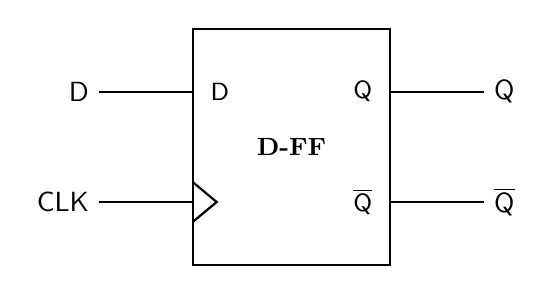
\begin{tikzpicture}[scale=1.0]
  % Ana dikdörtgen
  \draw[thick] (0,0) rectangle (2.5,3);

  % D girişi (sol üst)
  \draw[thick] (-1.2,2.2) -- (0,2.2);
  \node[left] at (-1.2,2.2) {\textsf{D}};
  \node[right, font=\small] at (0.1,2.2) {\textsf{D}};

  % CLK girişi (sol alt, üçgen sembolü)
  \draw[thick] (-1.2,0.8) -- (0,0.8);
  \node[left] at (-1.2,0.8) {\textsf{CLK}};
  \draw[thick] (0.0,0.55) -- (0.3,0.8) -- (0.0,1.05);

  % Q çıkışı (sağ üst)
  \draw[thick] (2.5,2.2) -- (3.7,2.2);
  \node[left, font=\small] at (2.4,2.2) {\textsf{Q}};
  \node[right] at (3.7,2.2) {\textsf{Q}};

  % Q-bar çıkışı (sağ alt)
  \draw[thick] (2.5,0.8) -- (3.7,0.8);
  \node[left, font=\small] at (2.4,0.8) {$\overline{\textsf{Q}}$};
  \node[right] at (3.7,0.8) {$\overline{\textsf{Q}}$};

  % Başlık
  \node[font=\small\bfseries] at (1.25,1.5) {D-FF};
\end{tikzpicture}
\caption{D türü flip-flop}
\label{fig:d-flip-flop}
\end{figure}

İşlemcinin verilerle çalışabilmesi için onları çok hızlı erişebildiği bir yerde tutması gerekir. Bellek bu iş için fazla yavaş kalır. İşte yazmaçlar, doğrudan işlemci içinde yer alan ve en hızlı erişilen veri saklama birimleridir. Örneğin RISC-V RV32I'de her biri 32 flip-floptan oluşan toplam 32 adet yazmaç bulunur. Sekiz flip-floptan oluşan 8 bitlik bir yazmaç örneği Şekil~\ref{fig:8bit-yazmac}'te gösterilmiştir. D flip-flopların çalışma ilkesi ve diğer ardışıl devre elemanları Ek~\ref{ch:sayisal-tasarim}'de (Bölüm~\ref{sec:ekB-yazmaclar}) ayrıntılı olarak ele alınmıştır.

Buradaki D flip-flop gösterimi, yazmacın kavramsal yapısını anlatmak içindir. Günümüz yüksek başarımlı işlemcilerinde yazmaç öbekleri genellikle SRAM tabanlı bit hücrelerinden oluşturulur; bu yapılar flip-floplara göre daha az alan kaplar ve çok kapılı (çok bağlantı noktalı) okuma/yazma erişimine olanak tanır. SRAM bit hücreleri bellek bölümünde ayrıntılı olarak incelenecektir.

\begin{figure}[H]
\centering
\begin{tikzpicture}[scale=1.0]
  % 8 adet D flip-flop yan yana
  \foreach \i in {0,...,7} {
    \pgfmathtruncatemacro{\bitno}{7-\i}
    % FF kutusu
    \draw[thick, fill=blokmavi-acik] (1.5*\i, 0) rectangle (1.5*\i+1.2, 2.0);
    \node[font=\tiny\bfseries] at (1.5*\i+0.6, 1.2) {D-FF};
    % Üstteki bit numarası (telin soluna kaydırılmış)
    \node[font=\tiny, above, anchor=south east, xshift=2pt] at (1.5*\i+0.6, 2.0) {Bit \bitno};
    % D girişi (üst — Q ile aynı boy: 0.5 birim)
    \draw[thick] (1.5*\i+0.6, 2.5) -- (1.5*\i+0.6, 2.0);
    \node[font=\scriptsize] at (1.5*\i+0.6, 2.7) {$D_{\bitno}$};
    % Q çıkışı (alt)
    \draw[thick] (1.5*\i+0.6, 0) -- (1.5*\i+0.6, -0.5);
    \node[font=\scriptsize] at (1.5*\i+0.6, -0.7) {$Q_{\bitno}$};
    % Saat üçgeni (kutunun sol alt köşesinde)
    \draw[thick] (1.5*\i, 0.15) -- (1.5*\i+0.25, 0.4) -- (1.5*\i, 0.65);
  }

  % Ortak saat hattı (sol tarafta dikey)
  \draw[thick, sinyalkirmizi] (-0.6, 0.4) -- (0, 0.4);
  \node[font=\small\bfseries, text=sinyalkirmizi, anchor=east] at (-0.7, 0.4) {Saat};
  % Saat bağlantıları (kutular arası yatay hat — son kutunun sol kenarında biter)
  \draw[thick, sinyalkirmizi] (0, 0.4) -- (10.5, 0.4);

  % Üst parantez - Veri Girişi (D etiketlerinin hemen üstünde)
  \draw[decorate, decoration={brace, amplitude=5pt, mirror}]
        (0.6, 3.0) -- (11.4, 3.0);
  \node[font=\small\bfseries] at (6.0, 3.25) {8 bitlik Veri Girişi};

  % Alt parantez - Veri Çıkışı
  \draw[decorate, decoration={brace, amplitude=5pt, raise=3pt}]
        (11.4, -0.8) -- (0.6, -0.8)
        node[midway, below=10pt, font=\small\bfseries] {8 bitlik Veri Çıkışı};
\end{tikzpicture}
\caption{8 bitlik veri tutan yazmaç (D flip-floplardan oluşan)}
\label{fig:8bit-yazmac}
\end{figure}

\subsection{Yazmaç Türleri}

\begin{itemize}
\item \textbf{Veri Yazmaçları:}\index{yazmaç!veri yazmacı} Tam sayı değerleri saklamak için kullanılırlar.
\item \textbf{Adres Yazmaçları:}\index{yazmaç!adres yazmacı} Bellekteki veriye ulaşmak için gerekli adresleri tutan yazmaçlardır.
\item \textbf{Genel Amaçlı Yazmaçlar:}\index{yazmaç!genel amaçlı} Her tür veriyi tutabildikleri için derleyici bu yazmaçları hem değişkenleri hem de adresleri saklamak için kullanabilir.
\item \textbf{Kayan Nokta Yazmaçları:}\index{yazmaç!kayan nokta} Ondalıklı sayıları tutmak için özel olarak tasarlanan yazmaçlardır.
\item \textbf{Sabit Değerli Yazmaçlar:}\index{yazmaç!sabit değerli} Yalnızca sabit değerleri tutar; üzerlerine yazılamaz.
\item \textbf{Vektör Yazmaçları:}\index{yazmaç!vektör} Çoklu ortam buyruklarının yaptığı vektör işlemleri için kullanılır.
\item \textbf{Özel Amaçlı Yazmaçlar:}\index{yazmaç!özel amaçlı} Program sayacı yazmacı gibi özel bir amaç için kullanılan yazmaçlardır.
\end{itemize}

\subsection{RISC-V'te Kullanılan Yazmaçlar}

RISC-V BKM'sinde 32 adet tam sayı yazmacı bulunur\index{RISC-V!yazmaçlar}. RISC-V'te yazmaçlar hem donanım adlarıyla (\texttt{x0}--\texttt{x31}) hem de ABI adlarıyla gösterilebilir; tüm yazmaçların adları ve görevleri Tablo~\ref{tab:riscv-yazmaclar}'da verilmiştir (ayrıca bkz.\ Ek~\ref{app:risc-v-referans}, Bölüm~\ref{sec:ekc-yazmaclar}).

\begin{table}[H]
\centering
\caption{RISC-V'te kullanılan yazmaçlar}
\label{tab:riscv-yazmaclar}
\small
\begin{tabular}{lllp{5.5cm}l}
\toprule
\textbf{ABI Adı} & \textbf{Donanım Adı} & \textbf{No} & \textbf{Kullanımı} & \textbf{Korunur?} \\
\midrule
\texttt{zero}      & \texttt{x0}      & 0     & Mutlak sıfır (her zaman 0)       & -- \\
\texttt{ra}        & \texttt{x1}      & 1     & Dönüş adresi                     & Hayır \\
\texttt{sp}        & \texttt{x2}      & 2     & Yığıt göstergesi                 & Evet \\
\texttt{gp}        & \texttt{x3}      & 3     & Genel gösterge                   & -- \\
\texttt{tp}        & \texttt{x4}      & 4     & İş parçacığı göstergesi          & -- \\
\texttt{t0}--\texttt{t2} & \texttt{x5}--\texttt{x7} & 5--7  & Geçici yazmaçlar          & Hayır \\
\texttt{s0/fp}     & \texttt{x8}      & 8     & Saklanan / Çerçeve göstergesi    & Evet \\
\texttt{s1}        & \texttt{x9}      & 9     & Saklanan yazmaç                  & Evet \\
\texttt{a0}--\texttt{a1} & \texttt{x10}--\texttt{x11} & 10--11 & Terim / Sonuç yazmaçları & Hayır \\
\texttt{a2}--\texttt{a7} & \texttt{x12}--\texttt{x17} & 12--17 & Terim yazmaçları         & Hayır \\
\texttt{s2}--\texttt{s11} & \texttt{x18}--\texttt{x27} & 18--27 & Saklanan yazmaçlar      & Evet \\
\texttt{t3}--\texttt{t6} & \texttt{x28}--\texttt{x31} & 28--31 & Geçici yazmaçlar        & Hayır \\
\bottomrule
\end{tabular}
\end{table}

\texttt{t} ile başlayan yazmaçlar (geçici) ve \texttt{s} ile başlayan yazmaçlar (saklanan) RISC-V'te genel amaçlı olarak kullanılır. Aralarındaki tek fark altyordam çağrılması sırasında \texttt{s} yazmaçlarının değerlerinin korunması, \texttt{t} yazmaçlarının ise değerlerinin korunmamasıdır.

\subsection{Özel Amaçlı Yazmaçlar}
\label{subsec:ozel-amacli-yazmaclar}
\index{yazmaç!özel amaçlı}\index{program sayacı}\index{CSR}

Tablo~\ref{tab:riscv-yazmaclar}'daki 32 genel amaçlı yazmacın yanı sıra, RISC-V mimarisinde programcının doğrudan erişemediği veya özel buyruklarla erişilen başka yazmaçlar da vardır. Bu yazmaçlar işlemcinin çalışma durumunu yönetir.

\subsubsection{Program Sayacı (PC)}
\index{program sayacı}

Program sayacı (\emph{program counter}, PC), o anda yürütülmekte olan buyruğun bellek adresini tutar. Her buyruk yürütüldükten sonra PC otomatik olarak 4 artar (çünkü RV32I'de her buyruk 4 bayt uzunluğundadır). Dallanma ve atlama buyrukları PC'yi farklı bir adrese yönlendirerek bu doğrusal akışı değiştirir.

``Program sayacı'' adı ilk bakışta yanıltıcı olabilir: bu yazmaç programları saymaz, \emph{program içinde} sayar; bellekteki buyrukları sırasıyla adresleyerek programın neresinde olduğumuzu takip eder. İlk bilgisayarlarda buyruklar ardışık bellek adreslerinde yer aldığından, bir sonraki buyruğa geçmek için bir sayaç yeterliydi ve bu yazmaç ``program sayacı'' adını aldı. Günümüzde PC bir sayaçtan çok bir \emph{adres göstergesidir}; ancak tarihsel ad yerleşmiştir.

PC, genel amaçlı yazmaç öbeğinın (\texttt{x0}--\texttt{x31}) bir parçası değildir; ayrı bir donanım yazmacıdır. Programcı PC'ye doğrudan bir değer yazamaz; PC yalnızca dallanma (\texttt{beq}, \texttt{bne}, \ldots), atlama (\texttt{jal}, \texttt{jalr}) ve kural dışı durum mekanizmaları aracılığıyla değişir. Ancak \texttt{auipc} buyruğu PC'nin o anki değerini \emph{okuyarak} bir yazmaçta kullanılabilir hale getirir; bu sayede konumdan bağımsız kod (\emph{position-independent code}) yazılabilir.

\begin{karsilastirma}[Program Sayacı: Farklı Mimarilerde Farklı Yaklaşımlar]
\index{buyruk işaretçisi}\index{instruction pointer|see{buyruk işaretçisi}}
Her mimari programın o anki konumunu izleyen bir yazmaca sahiptir; ancak adı, yapısı ve erişim biçimi farklılık gösterir.

\emph{RISC-V:} Ayrı bir donanım yazmacı olan PC, genel amaçlı yazmaç öbeğinın dışındadır. Doğrudan okunamaz ve yazılamaz; yalnızca \texttt{auipc} ile dolaylı okunabilir, dallanma/atlama buyrukları ile değiştirilebilir. Sabit 4 baytlık buyruklar nedeniyle her adımda $+4$ artar.

\emph{x86:} Intel bu yazmaca ``program sayacı'' değil, \emph{buyruk işaretçisi} (\emph{instruction pointer}) adını verir; 32 bitte \texttt{EIP}, 64 bitte \texttt{RIP}. Değişken uzunluklu buyruklar (1--15 bayt) nedeniyle artış miktarı her buyrukta farklıdır. Eski 16 bit modunda (8086) adres uzayı 1\,MB ile sınırlıydı; bu sınırı aşmak için \texttt{CS} (\emph{Code Segment}) yazmacı ile \texttt{IP} birlikte kullanılırdı: fiziksel adres $= \texttt{CS} \times 16 + \texttt{IP}$. Çağdaş 64 bit modunda bölütleme (\emph{segmentation}) işlevini yitirmiştir; \texttt{RIP} tek başına 64 bitlik sanal adresi tutar.

\emph{ARM AArch32:} Program sayacı, genel amaçlı yazmaç öbeğinın bir parçasıydı (\texttt{R15 = PC}). Bu tasarım, \texttt{ADD PC, PC, R0} gibi buyrukların doğrudan PC'ye yazmasına olanak tanıyordu; son derece esnekti ancak güvenlik açıklarına ve dallanma öngörücüsü karmaşıklığına yol açtı. ARM bu kararı AArch64'te düzeltti: PC artık ayrı bir yazmaçtır ve genel amaçlı buyruklar ile erişilemez.

\emph{MIPS:} RISC-V'e çok benzer biçimde PC ayrı bir yazmaçtır. Ancak MIPS'te bir ek karmaşıklık vardır: \emph{gecikmeli dallanma} (\emph{delayed branch}) nedeniyle dallanma buyruğundan \emph{sonraki} buyruk da yürütülür. RISC-V bu karmaşıklığı ortadan kaldırmıştır.
\end{karsilastirma}

\begin{bilginot}[PC Neden Genel Amaçlı Yazmaç Değildir?]
ARM AArch32'de program sayacının \texttt{R15} olarak genel amaçlı yazmaç öbeğina dahil edilmesi, başlangıçta zarif bir tasarım kararı gibi görünüyordu: herhangi bir buyruk PC'yi okuyabilir veya değiştirebilirdi. Ancak bu esneklik ciddi sorunlara yol açtı: (1)~güvenlik açıkları; bir saldırgan yazmaç üzerinden PC'yi keyfi bir adrese yönlendirebilirdi, (2)~dallanma öngörüsü karmaşıklığı; herhangi bir veri işleme buyruğu gizli bir dallanma olabilirdi, (3)~boru hattı tasarımı; PC'nin ne zaman güncelleneceği belirsizleşiyordu. Bu deneyimden ders çıkaran çağdaş mimariler (RISC-V, ARM AArch64, x86-64) PC'yi ayrı tutmayı tercih eder.
\end{bilginot}

\subsubsection{Denetim ve Durum Yazmaçları (CSR)}
\index{CSR}\index{denetim ve durum yazmacı}

RISC-V, işlemcinin çalışma durumunu ve ayrıcalık düzeyini yöneten özel yazmaçlara sahiptir. Bunlara \emph{denetim ve durum yazmaçları} (\emph{Control and Status Registers}, CSR) denir. CSR'lere genel amaçlı buyruklar (\texttt{add}, \texttt{lw} vb.) ile erişilemez; bunun yerine \texttt{csrrw}, \texttt{csrrs}, \texttt{csrrc} gibi özel CSR buyrukları kullanılır.

En sık karşılaşılan CSR yazmaçları Tablo~\ref{tab:csr-yazmaclari}'de listelenmiştir.

\begin{table}[H]
\centering
\caption[Temel CSR yazmaçları]{Temel denetim ve durum yazmaçları (CSR)}
\label{tab:csr-yazmaclari}
\small
\begin{tabular}{llp{7.5cm}}
\toprule
\texttt{CSR Adı} & Açılımı & Görevi \\
\midrule
\texttt{mstatus}  & Machine Status      & İşlemcinin çalışma durumunu tutar: kesmelerin açık/kapalı olduğu, önceki ayrıcalık düzeyi vb. \\
\texttt{mepc}     & Machine Exception PC & Kural dışı durum oluştuğunda PC'nin o anki değerini saklar. İşleyiciden dönüşte (\texttt{mret}) bu adrese geri dönülür. \\
\texttt{mcause}   & Machine Cause        & Kural dışı durumun nedenini belirten bir kod tutar (örneğin: geçersiz buyruk, sayfa hatası, zamanlayıcı kesmesi). \\
\texttt{mtvec}    & Machine Trap Vector  & Kural dışı durum işleyicisinin başlangıç adresini tutar. Bir kesme veya kural dışı durum oluştuğunda PC bu adrese yönlendirilir. \\
\texttt{mscratch} & Machine Scratch      & İşletim sistemi çekirdeğinin geçici veri saklayabileceği bir yazmaçtır. \\
\texttt{mhartid}  & Machine Hart ID      & Çok çekirdekli sistemlerde çekirdeğin kimlik numarasını tutar. \\
\midrule
\multicolumn{3}{l}{\emph{Başarım sayaçları}} \\
\midrule
\texttt{mcycle}    & Machine Cycle        & İşlemcinin başlatılmasından bu yana geçen saat çevrimi sayısını tutar. \\
\texttt{minstret}  & Machine Instructions Retired & İşlemcinin başlatılmasından bu yana tamamlanan buyruk sayısını tutar. \\
\bottomrule
\end{tabular}
\end{table}

CSR yazmaçları \emph{ayrıcalıklı} erişim gerektirir: \texttt{m} öneki ``makine'' (\emph{machine}) ayrıcalık düzeyini belirtir; bu, en yüksek yetki düzeyidir. Kullanıcı programları bu yazmaçlara doğrudan erişemez; erişim yalnızca işletim sistemi çekirdeği veya önyükleme yazılımı tarafından yapılır.

RISC-V'te üç ayrıcalık düzeyi tanımlanmıştır:

\begin{center}
\small
\begin{tabular}{cll}
\toprule
Düzey & Ad & Kullanım alanı \\
\midrule
0 & Kullanıcı (\emph{User}, U) & Uygulama programları \\
1 & Gözetmen (\emph{Supervisor}, S) & İşletim sistemi çekirdeği \\
3 & Makine (\emph{Machine}, M) & Donanım yazılımı, önyükleyici \\
\bottomrule
\end{tabular}
\end{center}

\texttt{ecall} buyruğu, bir alt düzeyden bir üst düzeye geçiş isteği göndermek için kullanılır. Örneğin kullanıcı düzeyindeki bir program \texttt{ecall} çalıştırdığında işlemci gözetmen veya makine düzeyine geçer; bu geçiş sırasında PC, \texttt{mtvec}'teki adrese yönlendirilir ve eski PC değeri \texttt{mepc}'ye kaydedilir. Bu mekanizmanın ayrıntıları Bölüm~9'da ele alınacaktır.

\begin{bilginot}[Başarım Sayaçları ve BBÇ Ölçümü]
\index{başarım sayacı}\index{mcycle}\index{minstret}
Tablo~\ref{tab:csr-yazmaclari}'deki \texttt{mcycle} ve \texttt{minstret} yazmaçları, Bölüm~\ref{chap:basarim}'deki başarım formülüyle doğrudan bağlantılıdır. Bu iki yazmacı okuyarak bir programın gerçek BBÇ değerini ölçebiliriz:
\[
\text{BBÇ} = \frac{\texttt{mcycle}}{\texttt{minstret}}
\]
Örneğin bir program çalıştırıldıktan sonra \texttt{mcycle}~$= 4200$ ve \texttt{minstret}~$= 3500$ okunursa BBÇ~$= 4200 / 3500 = 1{,}20$ olur; bu, ortalama olarak her buyruğun 1,2 çevrimde tamamlandığı anlamına gelir.

RISC-V, kullanıcı düzeyinden bu sayaçlara salt okunur erişim sağlayan \texttt{cycle} ve \texttt{instret} adlı gölge CSR'ler de tanımlar. Bu sayede ayrıcalıklı kipe geçmeden başarım ölçümü yapılabilir; ancak bu erişimin açık olup olmadığı \texttt{mcounteren} yazmacı ile denetlenir.

Donanım başarım sayaçları fikri RISC-V ile ortaya çıkmış değildir. Intel, 1993'te Pentium işlemcisiyle birlikte \emph{zaman damgası sayacı} (\emph{Time Stamp Counter}, TSC) adını verdiği 64 bitlik bir çevrim sayacını tanıttı; bu sayaç \texttt{RDTSC} buyruğuyla okunabiliyordu. Pentium Pro (1995) ile birlikte \emph{başarım izleme sayaçları} (\emph{Performance Monitoring Counters}, PMC) eklendi: önbellek bulma/bulamama oranları, dallanma öngörü başarısı, boru hattı duraklamaları gibi yüzlerce farklı olay sayılabilir hale geldi. Günümüzde Intel işlemcileri binlerce farklı donanım olayını izleyebilen programlanabilir sayaçlara sahiptir; Linux'taki \texttt{perf} aracı bu sayaçları kullanarak program başarımını ayrıntılı biçimde çözümler.

ARM da benzer bir altyapı sunar: ARMv7'den itibaren \emph{Başarım İzleyici Birimi} (\emph{Performance Monitor Unit}, PMU) standart bir bileşen olarak tanımlanmıştır. RISC-V'in farkı, en temel iki sayacı (\texttt{mcycle} ve \texttt{minstret}) zorunlu CSR olarak tanımlamasıdır; en basit RISC-V gerçeklemesinde bile bu sayaçlar bulunmalıdır.
\end{bilginot}

\begin{karsilastirma}[Özel Yazmaçlar: RISC-V, ARM ve x86]
Her mimari, genel amaçlı yazmaçların yanında özel amaçlı yazmaçlar tanımlar; ancak erişim yöntemleri farklıdır:

\emph{RISC-V:} Özel yazmaçlar (CSR) genel amaçlı yazmaç öbeğindan tamamen ayrıdır. Erişim yalnızca \texttt{csrrw}/\texttt{csrrs}/\texttt{csrrc} buyrukları ile yapılır. Bu ayrım tasarımı basitleştirir ve güvenliği artırır.

\emph{ARM AArch64:} Sistem yazmaçlarına \texttt{MSR}/\texttt{MRS} buyrukları ile erişilir. Yapı RISC-V'e benzer; ancak AArch32'de PC'nin genel amaçlı yazmaç (\texttt{R15}) olarak erişilebilmesi güvenlik sorunlarına yol açmıştır ve AArch64'te bu kaldırılmıştır.

\emph{x86-64:} Bayrak yazmacı (\texttt{RFLAGS}) aritmetik işlemlerin yan etkisi olarak otomatik güncellenir; ayrı bir buyrukla yazılmaz. Denetim yazmaçları (\texttt{CR0}--\texttt{CR4}) ve modele özgü yazmaçlar (MSR) ayrıcalıklı erişim gerektirir. Bayrak yazmacının varlığı, RISC-V'in bayrak yazmacı kullanmama kararıyla ilginç bir karşıtlık oluşturur.
\end{karsilastirma}

\subsubsection{Kayan Nokta Yazmaçları}
\index{yazmaç!kayan nokta}\index{RISC-V!kayan nokta yazmaçları}

RISC-V'in F (tek duyarlık) ve D (çift duyarlık) uzantıları etkinleştirildiğinde, tam sayı yazmaçlarından bağımsız 32 adet kayan nokta yazmacı (\texttt{f0}--\texttt{f31}) kullanılabilir hale gelir. Bu yazmaçlar ayrı bir yazmaç öbeğinda yer alır ve yalnızca kayan nokta buyrukları (\texttt{fadd.s}, \texttt{flw}, \texttt{fsw} vb.) ile erişilebilir.

Ayrıca kayan nokta işlemlerinin durumunu tutan bir denetim yazmacı (\texttt{fcsr}) bulunur. Bu yazmaç yuvarlama kipini ve kural dışı durum bayraklarını (taşma, sıfıra bölme vb.) içerir. Kayan nokta aritmetiğinin ayrıntıları Bölüm~5'te ele alınacaktır.

\begin{bilginot}[Yığıt Göstergesi: Donanım mı, Uzlaşı mı?]
\index{yığıt göstergesi}\index{RISC-V!yığıt göstergesi}
Tablo~\ref{tab:riscv-yazmaclar}'da \texttt{x2} yazmacının ABI adı \texttt{sp} (\emph{stack pointer}, yığıt göstergesi) olarak belirtilmişti. Ancak RISC-V donanımı açısından \texttt{x2} ile diğer yazmaçlar arasında hiçbir fark yoktur; \texttt{x2} sıradan bir genel amaçlı yazmaçtır. Yığıt göstergesi rolü tamamen yazılım uzlaşısına (ABI) dayanır; donanım \texttt{x2}'yi özel olarak tanımaz.

Bu, x86 ile temel bir farktır. x86'da \texttt{RSP} donanım düzeyinde özel bir yazmaçtır: \texttt{PUSH} buyruğu \texttt{RSP}'yi otomatik olarak azaltıp veriyi belleğe yazar; \texttt{POP} ise belekten okuyup \texttt{RSP}'yi artırır. \texttt{CALL} dönüş adresini \texttt{RSP}'nin gösterdiği yere yazar; \texttt{RET} oradan okur. Programcı \texttt{RSP}'yi başka amaçla kullansa bile bu buyruklar hâlâ \texttt{RSP}'yi yığıt göstergesi olarak varsayar.

RISC-V'te ise \texttt{PUSH}/\texttt{POP} buyrukları yoktur. Yığıta yazmak için programcı \texttt{sp}'yi açıkça güncelleyip \texttt{sw}/\texttt{lw} kullanır:
\begin{lstlisting}[style=riscv]
addi sp, sp, -4     # yer aç (PUSH'un birinci yarısı)
sw   t0, 0(sp)      # yığıta yaz (PUSH'un ikinci yarısı)
\end{lstlisting}
Bu yaklaşım daha fazla buyruk gerektirir; ancak donanımı sadeleştirir ve yazmaç öbeğinda özel durum mantığı gerektirmez. Aynı tasarım kararı \texttt{ra} (\texttt{x1}), \texttt{gp} (\texttt{x3}) ve \texttt{tp} (\texttt{x4}) için de geçerlidir; bunların hepsi donanım açısından sıradan yazmaçlardır, özel rolleri ABI tarafından atanmıştır.
\end{bilginot}

Şekil~\ref{fig:yazmac-haritasi}, RISC-V'teki tüm yazmaç türlerini ve aralarındaki ilişkiyi özetlemektedir.

\begin{figure}[H]
\centering
\begin{tikzpicture}[
    kutu/.style={draw, rounded corners=3pt, minimum width=3.2cm, minimum height=0.8cm, font=\small, align=center},
    baslik/.style={font=\small, anchor=south},
    okstil2/.style={->, >=stealth, thick}
]
% Genel amaçlı yazmaçlar
\node[kutu, fill=blokmavi-acik] (gp) at (0, 0) {x0 -- x31\\(32 $\times$ 32 bit)};
\node[baslik] at (0, 0.55) {Genel Amaçlı};

% Kayan nokta yazmaçları
\node[kutu, fill=blokyesil] (fp) at (4.5, 0) {f0 -- f31\\(32 $\times$ 32/64 bit)};
\node[baslik] at (4.5, 0.55) {Kayan Nokta};

% CSR
\node[kutu, fill=bloksari] (csr) at (9, 0) {mstatus, mepc,\\mcause, mtvec, \ldots};
\node[baslik] at (9, 0.55) {CSR};

% PC
\node[kutu, fill=blokkirmizi-acik] (pc) at (4.5, -2) {PC\\(32 bit)};

% fcsr
\node[kutu, fill=blokyesil!50] (fcsr) at (4.5, 1.8) {fcsr};

% Bağlantılar
\draw[okstil2, dashed] (pc.north west) -- node[left, font=\scriptsize, pos=0.4] {auipc} (gp.south east);
\draw[okstil2, dashed] (pc.north east) -- node[right, font=\scriptsize, pos=0.4] {jal, jalr} (csr.south west);
\draw[okstil2] (fcsr.south) -- (fp.north);

% Erişim buyrukları
\node[font=\scriptsize, text=gray, anchor=north] at (0, -0.55) {add, lw, sw, \ldots};
\node[font=\scriptsize, text=gray, anchor=north] at (4.5, -0.55) {fadd.s, flw, fsw, \ldots};
\node[font=\scriptsize, text=gray, anchor=north] at (9, -0.55) {csrrw, csrrs, csrrc};
\end{tikzpicture}
\caption[RISC-V yazmaç türleri]{RISC-V'teki yazmaç türleri ve erişim yöntemleri. Genel amaçlı, kayan nokta ve CSR yazmaçları birbirinden bağımsız dosyalarda yer alır. Program sayacı (PC) ayrı bir donanım yazmacıdır; dolaylı olarak okunabilir (\texttt{auipc}) ancak doğrudan yazılamaz.}
\label{fig:yazmac-haritasi}
\end{figure}

\subsection{Sıfır Yazmacı: x0 Neden Hep Sıfırdır}
\index{RISC-V!sıfır yazmacı}\index{x0 yazmacı}

Tablo~\ref{tab:riscv-yazmaclar}'da dikkat çeken bir ayrıntı, \texttt{x0} (\texttt{zero}) yazmacının değerinin her zaman sıfır olması ve üzerine yazılamamasıdır. Bu tasarım kararının ardında güçlü bir neden yatar: sıfır değeri programlarda son derece sık kullanılır ve ayrı bir sıfır yazmacı, pek çok işlemi ek buyruk gerektirmeden gerçekleştirmeyi sağlar. Örneğin:

\begin{itemize}[nosep]
\item Yazmaçtan yazmaca kopyalama: \texttt{add t0, t1, zero} $\equiv$ \texttt{mv t0, t1}
\item Koşulsuz atlama: \texttt{jal zero, etiket} $\equiv$ \texttt{j etiket} (dönüş adresi atılır)
\item Sonucu yok sayma: \texttt{jalr zero, rs1, 0} dönüş adresini kaydetmeden atlar
\item İşaret değiştirme: \texttt{sub t0, zero, t1} $\equiv$ \texttt{neg t0, t1}
\item Sıfırla karşılaştırma: \texttt{beq t0, zero, etiket} (t0 sıfır mı?)
\end{itemize}

Bu kullanımlar sayesinde ayrı \texttt{mov}, \texttt{nop}, \texttt{neg}, \texttt{j} buyrukları tanımlamaya gerek kalmaz; hepsi \texttt{x0} sayesinde mevcut buyrukların özel durumları olarak elde edilir. MIPS de aynı yaklaşımı benimser (\texttt{\$zero} yazmacı). ARM AArch64'te ise \texttt{XZR}/\texttt{WZR} yazmaçları benzer role sahiptir ancak aynı zamanda yığıt göstergesi (\texttt{SP}) olarak da kullanılabilir. x86'da böyle bir sıfır yazmacı yoktur; sıfır değeri gereken yerlerde anlık değer olarak belirtilmek zorundadır.

RISC-V'te terim yazmaçları \texttt{a0}--\texttt{a7} olarak toplam 8 adettir. Bu, MIPS'teki 4 terim yazmacından (\texttt{\$a0}--\texttt{\$a3}) daha fazladır ve altyordam çağrılarında daha fazla verinin yazmaçlar aracılığıyla geçirilmesine olanak tanır.

\subsection{RISC-V'te Neden Bayrak Yazmacı Yoktur?}
\label{subsec:bayrak-yazmaci}
\index{bayrak yazmacı}\index{RFLAGS|see{bayrak yazmacı}}\index{RISC-V!bayrak yazmacı yokluğu}

x86 ve ARM gibi mimarilerde aritmetik ve mantık buyrukları bir \emph{bayrak yazmacını} (\emph{flags register}) otomatik olarak güncellerler. Bu yazmaçtaki tek bitlik bayraklar, işlemin sonucuyla ilgili bilgi taşır:

\begin{center}
\small
\begin{tabular}{lll}
\toprule
Bayrak & Ad & Anlamı \\
\midrule
ZF & Zero Flag (Sıfır Bayrağı) & Sonuç sıfır mı? \\
CF & Carry Flag (Elde Bayrağı) & İşaretsiz taşma oluştu mu? \\
SF & Sign Flag (İşaret Bayrağı) & Sonuç negatif mi? \\
OF & Overflow Flag (Taşma Bayrağı) & İşaretli taşma oluştu mu? \\
\bottomrule
\end{tabular}
\end{center}

x86'da bir koşullu dallanma iki adımda gerçekleşir: önce \texttt{CMP} buyruğu bayrakları günceller, ardından \texttt{JE}, \texttt{JL} gibi bir koşullu atlama buyruğu bayrakları okuyarak karar verir:

\begin{lstlisting}[language={[x86masm]Assembler}, style=alistirma-kod]
CMP  EAX, EBX    ; EAX - EBX hesapla, bayraklari guncelle
JGE  buyuk       ; SF=OF ise (>= durumu) atla
\end{lstlisting}

RISC-V ise bayrak yazmacı kullanmaz. Bunun yerine karşılaştırma ve dallanma tek bir buyrukta birleştirilir:

\begin{lstlisting}[style=riscv]
bge  t0, t1, buyuk   # t0 >= t1 ise dallan
\end{lstlisting}

Bu tasarım kararının arkasında üç önemli neden vardır:

\begin{enumerate}
\item \emph{Bağımlılık zincirini kırmak:} Bayrak yazmacı tek bir ortak kaynaktır. Ardışık buyrukların hepsi aynı bayrak yazmacını okuyup yazarsa, bu buyruklar birbirine bağımlı hale gelir ve koşut yürütülmeleri zorlaşır. Bayrak yazmacı olmadığında her buyruk yalnızca kendi hedef yazmacını yazar; bağımsız buyruklar koşut biçimde yürütülebilir.

\item \emph{Sırasız yürütümü kolaylaştırmak:} Çağdaş yüksek başarımlı işlemciler buyrukları program sırasından farklı bir düzende yürütebilir (\emph{out-of-order execution}). Bayrak yazmacı bu esnekliği kısıtlar çünkü bayrakları güncelleyen ve okuyan buyruklar arasındaki sıra korunmalıdır. RISC-V'te bu sorun yoktur; karşılaştırma ve dallanma aynı buyrukta yapılır.

\item \emph{Tasarımı sadeleştirmek:} Bayrak yazmacının güncelleme ve okuma mantığı, boru hattı tasarımına ek karmaşıklık getirir. Hangi buyruğun bayrakları güncellediği, hangisinin yalnızca okuduğu izlenmelidir. RISC-V bu karmaşıklığı ortadan kaldırarak donanım tasarımını sadeleştirir.
\end{enumerate}

\begin{karsilastirma}[Dallanma Mekanizması: Bayraklı ve Bayraksız Mimariler]
\emph{x86 (bayraklı):} Karşılaştırma (\texttt{CMP}) ve dallanma (\texttt{JGE}) iki ayrı buyruktur. Arada başka buyruklar bayrakları bozabilir; derleyicinin bu durumu dikkatle yönetmesi gerekir. Avantajı: tek bir karşılaştırma sonucunu birden çok dallanma buyruğu kullanabilir.

\emph{ARM (bayraklı, seçimli):} AArch32'de yalnızca sonuna \texttt{S} eklenen buyruklar (\texttt{ADDS}, \texttt{SUBS}) bayrakları günceller; \texttt{ADD}, \texttt{SUB} güncellemez. Bu, x86'nın ``her buyruk bayrak günceller'' sorununu kısmen çözer. AArch64'te ayrıca \texttt{CBZ}/\texttt{CBNZ} gibi bayraksız dallanma buyrukları da eklenmiştir.

\emph{RISC-V (bayraksız):} \texttt{beq}, \texttt{bne}, \texttt{blt}, \texttt{bge}, \texttt{bltu}, \texttt{bgeu} buyrukları iki yazmacı doğrudan karşılaştırıp dallanır. Bayrak yazmacı olmadığı için ardışık buyruklar arasında gizli bağımlılık oluşmaz. Dezavantajı: aynı karşılaştırma sonucunu birden çok dallanma kullanmak istiyorsa karşılaştırma tekrarlanmalıdır; ancak bu durum uygulamada nadirdir.

\emph{MIPS (bayraksız):} RISC-V'e benzer biçimde \texttt{beq}/\texttt{bne} buyrukları kullanır; ancak ``küçükse'' karşılaştırması için ayrı bir \texttt{slt} (set on less than) buyruğu ile sonucu bir yazmaca yazıp ardından \texttt{bne} ile dallanma gerekir: iki buyruk. RISC-V'in \texttt{blt} buyruğu bu işi tek buyrukta yapar.
\end{karsilastirma}

\subsection{Yazmaç Sayısı ve Tasarım Dengeleri}
\label{subsec:yazmac-sayisi-dengesi}
\index{yazmaç!sayısı}\index{yazmaçtan belleğe taşıma}

Farklı mimarilerin yazmaç sayıları arasında büyük farklar vardır. Bu fark rastlantısal değildir; yazmaç sayısı hem başarımı hem de buyruk kodlama biçimini doğrudan etkiler.

\begin{table}[H]
\centering
\caption{Dört mimaride yazmaç karşılaştırması}
\label{tab:yazmac-karsilastirma}
\small
\begin{tabular}{lccll}
\toprule
\textbf{Mimari} & \textbf{Genel Amaçlı} & \textbf{Genişlik} & \textbf{Adlandırma} & \textbf{Özel Yazmaçlar} \\
\midrule
RISC-V (RV32I) & 32 & 32 bit & \texttt{x0}--\texttt{x31} & \texttt{x0} = sıfır \\
RISC-V (RV64I) & 32 & 64 bit & \texttt{x0}--\texttt{x31} & \texttt{x0} = sıfır \\
MIPS            & 32 & 32 bit & \texttt{\$0}--\texttt{\$31} & \texttt{\$0} = sıfır, HI/LO \\
ARM (AArch64)   & 31 & 64 bit & \texttt{X0}--\texttt{X30} & XZR/SP (bağlama göre) \\
x86 (IA-32)     & 8  & 32 bit & \texttt{EAX}--\texttt{EDI} & Örtük roller \\
x86-64          & 16 & 64 bit & \texttt{RAX}--\texttt{R15} & Örtük roller \\
\bottomrule
\end{tabular}
\end{table}

Tablo~\ref{tab:yazmac-karsilastirma}'de görüldüğü gibi mimari tasarımlar arasında yazmaç sayısı önemli ölçüde farklılık gösterir. Her iki uçtaki sorunları anlamak, mimari tasarım kararlarının ardındaki mantığı kavramak açısından önemlidir.

Yazmaç sayısı az olduğunda derleyici, hesaplama sırasında kullanılan tüm değişkenleri yazmaçlarda tutamaz. Bu durumda bazı değerleri geçici olarak belleğe (yığıta) yazmak ve daha sonra geri okumak zorunda kalır. Bu işleme \emph{yazmaçtan belleğe taşıma}\index{yazmaçtan belleğe taşıma} (\emph{register spilling}) denir; bu duruma yol açan yetersizliğe de \emph{yazmaç yetersizliği}\index{yazmaç yetersizliği} adı verilir. Derleyici, yazmaca sığdıramadığı her değer için fazladan bir saklama (\texttt{store}) ve bir yükleme (\texttt{load}) buyruğu üretmek zorundadır; bu da hem buyruk sayısını artırır hem de yavaş bellek erişimleri nedeniyle başarımı düşürür. Örneğin x86 IA-32'nin yalnızca 8 genel amaçlı yazmacı olması, derleyicileri sık sık yazmaçtan belleğe taşıma yapmaya zorlamış ve bu durum x86-64'te yazmaç sayısının 16'ya çıkarılmasının başlıca nedenlerinden biri olmuştur.

Öte yandan yazmaç sayısını artırmanın da bir bedeli vardır. Her buyrukta kaynak ve hedef yazmaçlarını belirtmek için daha fazla bit gerekir: 32 yazmaç, buyrukta yazmaç numarasını kodlamak için 5 bit gerektirirken, 16 yazmaç 4 bit, 8 yazmaç ise 3 bit gerektirir. Üç yazmaçlı bir buyrukta (kaynak~1, kaynak~2, hedef) bu fark $3 \times (5 - 3) = 6$ bite ulaşır. Sabit 32 bitlik buyruk genişliğinde bu fazladan bitler, anlık değerler ve işlem kodları için ayrılabilecek alandan çalınır. Aynı programın makine kodu daha fazla yer kaplar ve buyruk önbelleğine (\emph{instruction cache}) daha fazla baskı uygular; bu duruma \emph{kod şişmesi}\index{kod şişmesi} (\emph{code bloat}) denir.

Bağlam değiştirme (\emph{context switch}) maliyeti de yazmaç sayısıyla doğru orantılıdır. İşletim sistemi bir süreçten diğerine geçerken tüm yazmaçların belleğe kaydedilip geri yüklenmesi gerekir; 32 yazmaçlı bir mimaride bu işlem, 8 yazmaçlı bir mimariye göre dört kat daha fazla veri aktarımı gerektirir.

\newcommand{\artii}{\textcolor{green!60!black}{\ding{51}}\;}
\newcommand{\eksii}{\textcolor{red!70!black}{\ding{55}}\;}

\begin{table}[H]
\centering
\caption{Yazmaç sayısının artı ve eksileri}
\label{tab:yazmac-sayisi-dengeleri}
\small
\begin{tabular}{p{3.2cm}p{5.3cm}p{5.3cm}}
\toprule
 & \textbf{Az yazmaç} (ör.\ x86 IA-32: 8) & \textbf{Çok yazmaç} (ör.\ RISC-V: 32) \\
\midrule
Buyruk genişliği & \artii Yazmaç numarası az bit tutar $\rightarrow$ anlık değerlere ve işlem koduna daha fazla alan kalır & \eksii Yazmaç numarası çok bit tutar $\rightarrow$ sabit genişlikli buyrukta alan daralır \\[4pt]
Kod boyutu & \artii Daha küçük buyruklar $\rightarrow$ buyruk önbelleği verimli & \eksii Daha geniş buyruklar $\rightarrow$ kod şişmesi riski \\[4pt]
Bellek erişimi & \eksii Yazmaç yetmez $\rightarrow$ yazmaçtan belleğe taşıma sık $\rightarrow$ yavaş & \artii Değerler yazmaçlarda kalır $\rightarrow$ az bellek erişimi $\rightarrow$ hızlı \\[4pt]
Yazmaç erişim gecikmesi & \artii Yazmaç dosyası küçük $\rightarrow$ okuma/yazma süresi kısa; yüksek saat hızını destekler & \eksii Yazmaç dosyası büyük $\rightarrow$ okuma/yazma bağlantı noktaları artar, fiziksel erişim süresi uzar; saat döngüsünü sınırlayabilir \\[4pt]
Derleyici karmaşıklığı & \eksii Yazmaç ataması zor; belleğe taşıma yönetimi gerekli & \artii Yazmaç ataması kolay; boş yazmaç bulmak daha olası \\[4pt]
Bağlam değiştirme & \artii Az yazmaç kaydedilir $\rightarrow$ hızlı & \eksii Çok yazmaç kaydedilir $\rightarrow$ yavaş \\[4pt]
Donanım maliyeti & \artii Yazmaç dosyası küçük $\rightarrow$ az alan ve güç & \eksii Yazmaç dosyası büyük $\rightarrow$ daha fazla alan ve güç \\
\bottomrule
\end{tabular}

\medskip
\footnotesize
\textcolor{green!60!black}{\ding{51}}~=~o seçenek için avantaj \quad
\textcolor{red!70!black}{\ding{55}}~=~o seçenek için dezavantaj
\end{table}

Tablo~\ref{tab:yazmac-sayisi-dengeleri}'de özetlendiği gibi, az ve çok yazmaç arasında bir denge noktası vardır. Aşağıdaki iki örnek bu dengeyi somut olarak göstermektedir.

\begin{terimnotu}
\textbf{yazmaçtan belleğe taşıma} (\emph{register spilling})\,: İngilizcede \emph{register spilling} terimi, ``taşma'' ve ``dökülme'' çağrışımı taşır; tıpkı dolan bir tabaktan sulu yemeğin taşması gibi, yazmaçlara sığmayan değerler belleğe ``dökülür.'' Türkçede bu mecaz doğal karşılanmadığından, kavramı daha açık ifade eden \emph{yazmaçtan belleğe taşıma} veya kısaca \emph{yazmaç boşaltma} karşılıkları tercih edilmektedir. Derleyici, hesaplama sırasında kullanılan tüm değişkenleri yazmaçlarda tutamadığında bazı değerleri geçici olarak belleğe (genellikle yığıta) yazar ve ihtiyaç duyulduğunda geri yükler. Bu işlem fazladan saklama (\texttt{store}) ve yükleme (\texttt{load}) buyrukları üretir; hem buyruk sayısını artırır hem de yavaş bellek erişimleri nedeniyle başarımı düşürür.
\end{terimnotu}

\begin{ornek}[3.3]
\label{orn:yazmac-tasima}
Aşağıdaki C ifadesini ele alalım:

\begin{lstlisting}[language=C]
int a = b + c - d * e + f;
\end{lstlisting}

Bu ifade derlendiğinde beş farklı değişken (\texttt{b}, \texttt{c}, \texttt{d}, \texttt{e}, \texttt{f}) eş zamanlı olarak kullanımdadır. Derleyicinin bunları yazmaçlarda nasıl yönettiği, mimarinin sunduğu yazmaç sayısına bağlıdır.

\textbf{Çözüm:}

\textbf{(a) 8 yazmaçlı mimari (x86 IA-32 benzeri):}

x86 IA-32'de yalnızca 8 genel amaçlı yazmaç bulunur; ancak bazıları örtük rollere sahip olduğundan derleyiciye en fazla 5--6 yazmaç kalır. Beş değişken aynı anda gerektiğinde derleyici bir ya da iki değeri yığıta taşımak zorunda kalır. Bunun sonucunda üretilen kod şuna benzer:

\begin{lstlisting}[language={}, morecomment={[l]{;}}, texcl=true]
; x86 IA-32 benzeri (basitleştirilmiş)
; Yazmaçlar: EAX, ECX, EDX, EBX (4 yazmaç mevcut)
; d ve e yığıta alınıyor (yazmaçtan belleğe taşıma kodu):
    mov  [esp-4], d_val    ; store: d'yi yığıta yaz
    mov  [esp-8], e_val    ; store: e'yi yığıta yaz
    mov  EAX, b            ; EAX = b
    add  EAX, c            ; EAX = b + c
    mov  ECX, [esp-4]      ; load: d'yi yığıttan geri oku
    imul ECX, [esp-8]      ; load: ECX = d * e (e yığıttan)
    sub  EAX, ECX          ; EAX = b + c - d*e
    add  EAX, f            ; EAX = b + c - d*e + f
    mov  [a], EAX          ; a'yı belleğe yaz
\end{lstlisting}

Toplam: 2 fazladan saklama (\texttt{store}) + 2 fazladan yükleme (\texttt{load}) = 4 fazladan bellek erişim buyruğu.

\textbf{(b) 32 yazmaçlı mimari (RISC-V):}

RISC-V'te 32 genel amaçlı yazmaç bulunur. Beş değişken kolayca ayrı yazmaçlara atanır; yığıta taşıma gerekmez:

\begin{lstlisting}[style=riscv]
# t0=b, t1=c, t2=d, t3=e, t4=f; s0 a değişkeninin adresi
add  t5, t0, t1        # t5 = b + c
mul  t6, t2, t3        # t6 = d * e
sub  t5, t5, t6        # t5 = b + c - d*e
add  t5, t5, t4        # t5 = b + c - d*e + f
sw   t5, 0(s0)         # sonucu belleğe yaz
\end{lstlisting}

Toplam: 0 fazladan saklama/yükleme buyruğu (yalnızca son sonuç belleğe yazılır).

\medskip
\textbf{Sonuç:} 8 yazmaçlı mimaride toplam 9 buyruk (4'ü belleğe taşıma kodu), 32 yazmaçlı mimaride ise 5 buyruk yeterlidir. Bu fark yalnızca buyruk sayısını değil, Bölüm~\ref{chap:basarim}'deki yürütme zamanı denkleminin (Denklem~\ref{eq:yurutme-zamani-bbc}) her üç bileşenini de etkiler:

\begin{itemize}[nosep]
\item \emph{Buyruk sayısı azalır:} 32 yazmaçlı mimaride belleğe taşıma buyrukları ortadan kalktığından toplam buyruk sayısı düşer.
\item \emph{BBÇ düşer:} Eklenen her \texttt{lw}/\texttt{sw} buyruğu belleğe erişir; önbellekte bulamama durumunda tek bir yükleme onlarca saat döngüsü sürebilir. Yazmaç erişimi ise tek döngüde tamamlanır. Bellek buyruklarının oranı azaldıkça ortalama BBÇ de düşer.
\item \emph{Çevrim zamanı artabilir:} Yazmaç dosyası büyüdükçe fiziksel erişim gecikmesi uzar; bu durum saat döngüsünü sınırlayabilir. Ancak günümüz teknolojisinde 32 yazmaçlı bir dosyanın erişim süresi genellikle tek döngüde kalır.
\end{itemize}

Gerçek derleyicilerde bu fark, özellikle döngü gövdelerinde sürekli yinelenerek toplam başarım üzerinde belirgin bir etki bırakır. Bir sonraki örnekte bu etkiyi sayısal olarak hesaplayacağız.
\end{ornek}

\begin{ornek}[3.4]
\label{orn:yazmac-basarim}
Örnek~3.3'teki iki mimariyi karşılaştıralım. Aşağıdaki varsayımları kullanarak her iki mimarideki yürütme zamanını hesaplayın ve hangisinin daha hızlı olduğunu bulun.

\begin{itemize}[nosep]
\item 8 yazmaçlı mimari: 9 buyruk (4'ü bellek erişimi), saat sıklığı 4{,}0~GHz.
\item 32 yazmaçlı mimari: 5 buyruk (yalnızca 1 bellek erişimi), saat sıklığı 3{,}8~GHz (daha büyük yazmaç öbeği nedeniyle biraz düşük).
\item Aritmetik buyruklar 1 çevrim, bellek buyrukları (\texttt{lw}/\texttt{sw}) ortalama 3 çevrim sürüyor (önbellek etkisi dahil).
\end{itemize}

\textbf{Çözüm:}

Denklem~\ref{eq:yurutme-zamani-bbc}'yi kullanıyoruz: $\text{Yürütme zamanı} = \text{Buyruk sayısı} \times \text{BBÇ} \times \text{Çevrim zamanı}$.

\medskip
\textbf{(a) 8 yazmaçlı mimari:}

9 buyruktan 5'i aritmetik (1 çevrim), 4'ü bellek (3 çevrim):
\[
\text{Toplam çevrim} = 5 \times 1 + 4 \times 3 = 17 \quad\Rightarrow\quad \text{BBÇ} = \frac{17}{9} \approx 1{,}89
\]
\[
\text{Yürütme zamanı} = \frac{17}{4{,}0 \times 10^{9}} = 4{,}25 \text{ ns}
\]

\textbf{(b) 32 yazmaçlı mimari:}

5 buyruktan 4'ü aritmetik (1 çevrim), 1'i bellek (3 çevrim):
\[
\text{Toplam çevrim} = 4 \times 1 + 1 \times 3 = 7 \quad\Rightarrow\quad \text{BBÇ} = \frac{7}{5} = 1{,}40
\]
\[
\text{Yürütme zamanı} = \frac{7}{3{,}8 \times 10^{9}} = 1{,}84 \text{ ns}
\]

\textbf{Sonuç:} 32 yazmaçlı mimari $4{,}25 / 1{,}84 = 2{,}31$ kat daha hızlıdır; saat hızının \%5 düşük olmasına karşın. Kazanç iki kaynaktan gelir: buyruk sayısı 9'dan 5'e düşmüştür (belleğe taşıma buyrukları ortadan kalkmıştır) ve bellek buyrukları oranı azaldığından ortalama BBÇ 1{,}89'dan 1{,}40'a gerilemiştir. Bu örnek, yazmaç sayısı artışının çevrim zamanındaki küçük kaybı fazlasıyla telafi edebildiğini göstermektedir.
\end{ornek}

\begin{ornek}[3.5]
16 bitlik sabit genişlikli buyruk kullanan bir işlemci tasarladığınızı düşünün. Y (Yazmaç) türü buyruklar (ör.\ \texttt{add rd, rs1, rs2}) üç yazmaç numarası ve bir işlem kodu alanı içermelidir. A (Anlık) türü buyruklar (ör.\ \texttt{addi rd, rs1, 5}) ise iki yazmaç numarası, bir işlem kodu ve bir anlık değer alanı taşımalıdır. İşlem kodu her iki türde de 4 bit olsun. Yazmaç sayısını sırasıyla 8, 16 ve 32 olarak seçtiğinizde kalan bit sayılarını hesaplayın.

\textbf{Çözüm:}

\begin{figure}[H]
\centering
\begin{tikzpicture}[scale=0.75]
  \def\bw{0.8}  % bit genişliği
  \def\yuk{0.7} % yükseklik

  % === (a) 8 yazmaç — Y türü ===
  \node[font=\small\bfseries, anchor=west] at (-0.5, 4.8) {(a) 8 yazmaç — Y türü};
  % opcode 4 bit
  \draw[thick, fill=blokmavi] (0, 3.8) rectangle (4*\bw, 3.8+\yuk);
  \node[font=\tiny\bfseries] at (2*\bw, 3.8+\yuk/2+0.1) {işlem kodu};
  \node[font=\tiny] at (2*\bw, 3.8+\yuk/2-0.15) {\strut 4 bit};
  % rd 3 bit
  \draw[thick, fill=bloksari] (4*\bw, 3.8) rectangle (7*\bw, 3.8+\yuk);
  \node[font=\tiny\bfseries] at (5.5*\bw, 3.8+\yuk/2+0.1) {rd};
  \node[font=\tiny] at (5.5*\bw, 3.8+\yuk/2-0.15) {\strut 3 bit};
  % rs1 3 bit
  \draw[thick, fill=blokyesil] (7*\bw, 3.8) rectangle (10*\bw, 3.8+\yuk);
  \node[font=\tiny\bfseries] at (8.5*\bw, 3.8+\yuk/2+0.1) {rs1};
  \node[font=\tiny] at (8.5*\bw, 3.8+\yuk/2-0.15) {\strut 3 bit};
  % rs2 3 bit
  \draw[thick, fill=blokyesil] (10*\bw, 3.8) rectangle (13*\bw, 3.8+\yuk);
  \node[font=\tiny\bfseries] at (11.5*\bw, 3.8+\yuk/2+0.1) {rs2};
  \node[font=\tiny] at (11.5*\bw, 3.8+\yuk/2-0.15) {\strut 3 bit};
  % boş 3 bit
  \draw[thick, fill=gray!15, pattern=north east lines, pattern color=gray!40] (13*\bw, 3.8) rectangle (16*\bw, 3.8+\yuk);
  \node[font=\tiny] at (14.5*\bw, 3.8+\yuk/2+0.1) {boş};
  \node[font=\tiny] at (14.5*\bw, 3.8+\yuk/2-0.15) {\strut 3 bit};
  % toplam (alt parantez — kutudan aşağıda)
  \draw[decorate, decoration={brace, amplitude=4pt, raise=4pt, mirror}]
        (0, 3.8) -- (16*\bw, 3.8)
        node[midway, below=10pt, font=\tiny\bfseries] {16 bit};

  % === (b) 16 yazmaç — Y türü ===
  \node[font=\small\bfseries, anchor=west] at (-0.5, 2.5) {(b) 16 yazmaç — Y türü};
  % opcode 4 bit
  \draw[thick, fill=blokmavi] (0, 1.5) rectangle (4*\bw, 1.5+\yuk);
  \node[font=\tiny\bfseries] at (2*\bw, 1.5+\yuk/2+0.1) {işlem kodu};
  \node[font=\tiny] at (2*\bw, 1.5+\yuk/2-0.15) {\strut 4 bit};
  % rd 4 bit
  \draw[thick, fill=bloksari] (4*\bw, 1.5) rectangle (8*\bw, 1.5+\yuk);
  \node[font=\tiny\bfseries] at (6*\bw, 1.5+\yuk/2+0.1) {rd};
  \node[font=\tiny] at (6*\bw, 1.5+\yuk/2-0.15) {\strut 4 bit};
  % rs1 4 bit
  \draw[thick, fill=blokyesil] (8*\bw, 1.5) rectangle (12*\bw, 1.5+\yuk);
  \node[font=\tiny\bfseries] at (10*\bw, 1.5+\yuk/2+0.1) {rs1};
  \node[font=\tiny] at (10*\bw, 1.5+\yuk/2-0.15) {\strut 4 bit};
  % rs2 4 bit
  \draw[thick, fill=blokyesil] (12*\bw, 1.5) rectangle (16*\bw, 1.5+\yuk);
  \node[font=\tiny\bfseries] at (14*\bw, 1.5+\yuk/2+0.1) {rs2};
  \node[font=\tiny] at (14*\bw, 1.5+\yuk/2-0.15) {\strut 4 bit};
  % toplam (alt parantez — kutudan aşağıda)
  \draw[decorate, decoration={brace, amplitude=4pt, raise=4pt, mirror}]
        (0, 1.5) -- (16*\bw, 1.5)
        node[midway, below=10pt, font=\tiny\bfseries] {16 bit — tam sığar};

  % === (c) 32 yazmaç — Y türü ===
  \node[font=\small\bfseries, anchor=west] at (-0.5, 0.2) {(c) 32 yazmaç — Y türü};
  % opcode 4 bit
  \draw[thick, fill=blokmavi] (0, -0.8) rectangle (4*\bw, -0.8+\yuk);
  \node[font=\tiny\bfseries] at (2*\bw, -0.8+\yuk/2+0.1) {işlem kodu};
  \node[font=\tiny] at (2*\bw, -0.8+\yuk/2-0.15) {\strut 4 bit};
  % rd 5 bit
  \draw[thick, fill=bloksari] (4*\bw, -0.8) rectangle (9*\bw, -0.8+\yuk);
  \node[font=\tiny\bfseries] at (6.5*\bw, -0.8+\yuk/2+0.1) {rd};
  \node[font=\tiny] at (6.5*\bw, -0.8+\yuk/2-0.15) {\strut 5 bit};
  % rs1 5 bit
  \draw[thick, fill=blokyesil] (9*\bw, -0.8) rectangle (14*\bw, -0.8+\yuk);
  \node[font=\tiny\bfseries] at (11.5*\bw, -0.8+\yuk/2+0.1) {rs1};
  \node[font=\tiny] at (11.5*\bw, -0.8+\yuk/2-0.15) {\strut 5 bit};
  % rs2 5 bit — taşar!
  \draw[thick, fill=blokkirmizi, fill opacity=0.3] (14*\bw, -0.8) rectangle (19*\bw, -0.8+\yuk);
  \node[font=\tiny\bfseries] at (16.5*\bw, -0.8+\yuk/2+0.1) {rs2};
  \node[font=\tiny] at (16.5*\bw, -0.8+\yuk/2-0.15) {\strut 5 bit};
  % 16 bit sınırı (kesikli çizgi + üstünde ortalanmış yazı)
  \draw[very thick, sinyalkirmizi, dashed] (16*\bw, -1.1) -- (16*\bw, 0.2);
  \node[font=\tiny\bfseries, text=sinyalkirmizi, anchor=south] at (16*\bw, 0.25) {16 bit sınırı};
  % toplam 19 bit (alt parantez — kutudan aşağıda)
  \draw[decorate, decoration={brace, amplitude=4pt, raise=4pt, mirror}]
        (0, -0.8) -- (19*\bw, -0.8)
        node[midway, below=10pt, font=\tiny\bfseries, text=sinyalkirmizi] {19 bit — sığmaz!};
\end{tikzpicture}
\caption{16 bitlik buyruklarda yazmaç sayısının etkisi (Y türü buyruklar)}
\label{fig:yazmac-sayisi-etkisi}
\end{figure}

\begin{table}[H]
\centering
\small
\begin{tabular}{lccccc}
\toprule
 & \textbf{Yazmaç} & \textbf{Yazmaç num.} & \multicolumn{2}{c}{\textbf{Y türü (3 yazmaç)}} & \textbf{A türü (2 yazmaç)} \\
 & \textbf{sayısı} & \textbf{(bit)} & \textbf{Toplam} & \textbf{Kalan} & \textbf{Anlık değer (bit)} \\
\midrule
(a) & 8  & 3 & $4 + 3\!\times\!3 = 13$ & 3 bit boş & $16 - 4 - 3\!\times\!2 = 6$ bit $(\pm 32)$ \\
(b) & 16 & 4 & $4 + 3\!\times\!4 = 16$ & 0 bit $\checkmark$ & $16 - 4 - 4\!\times\!2 = 4$ bit $(\pm 8)$ \\
(c) & 32 & 5 & $4 + 3\!\times\!5 = 19$ & \textbf{sığmaz!} & $16 - 4 - 5\!\times\!2 = 2$ bit $(\pm 2)$ \\
\bottomrule
\end{tabular}
\end{table}

Şekil~\ref{fig:yazmac-sayisi-etkisi}'de Y türü buyrukların bit dağılımı görselleştirilmiştir.
\begin{itemize}[nosep]
\item 8 yazmaçla (a) her şey rahatça sığar; anlık değer alanı 6 bit olup $-32$'den $+31$'e kadar bir aralığı ifade edebilir.
\item 16 yazmaçla (b) Y türü buyruk 16 bitin tamamını doldurur, hiç boş bit kalmaz. Anlık değer alanı ise 4 bite düşer; artık yalnızca $-8$'den $+7$'ye kadar bir aralık gösterilebilir. Daha büyük sabitler için ek buyruklar gerekir.
\item 32 yazmaçla (c) Y türü buyruk 19 bit gerektirir; 16 bite sığmaz. A türünde anlık değer alanı yalnızca 2 bit kalır ($-2$'den $+1$'e); bu da neredeyse kullanışsızdır.
\end{itemize}

Bu örnek, RISC-V'in neden 32 bitlik buyruk genişliği seçtiğini ve RISC-V C (sıkıştırılmış) uzantısının 16 bitlik buyruklarda yazmaç sayısını 8'e düşürmek zorunda kaldığını açıkça göstermektedir.
\end{ornek}

Günümüz mimarilerinin çoğu 16--32 aralığında bir yazmaç sayısıyla bu dengeyi kurmaktadır. x86'nın 8 yazmacı yetersiz kalmış, x86-64'te 16'ya çıkarılmıştır. RISC-V ve MIPS'in 32 yazmacı ise derleyicilere yeterli esnekliği sağlarken buyruk kodlama genişliğini kabul edilebilir sınırlarda tutmaktadır.

\begin{karsilastirma}[Yazmaç Yapıları]
RISC-V 32 adet genel amaçlı tam sayı yazmacına sahiptir; \texttt{x0} donanım tarafından sıfıra sabitlenmiştir ve üzerine yazılamaz. MIPS de 32 yazmaç sunar (\texttt{\$0} = sıfır); ancak çarpma ve bölme sonuçları için ayrı HI ve LO yazmaçları bulunur ve bunlara erişmek için özel \texttt{mfhi}/\texttt{mflo} buyruklarına gerek duyulur. RISC-V bu durumu M uzantısıyla genel amaçlı yazmaçlara yazarak çözmüştür.

ARM (AArch64) 31 adet genel amaçlı yazmaç (X0--X30) ile birlikte yazmaç konumuna göre sıfır ya da yığıt göstergesi gibi davranan XZR/SP rolüne sahiptir; bu da etkin olarak 32 konuma karşılık gelir.

x86-64 ise yalnızca 16 genel amaçlı yazmaç sunar (RAX--R15). IA-32'de bu sayı 8'di. Üstelik bazı yazmaçların örtük rolleri vardır: RCX döngü sayacı, RSP yığıt göstergesi, RAX çarpma/bölme sonucu, RDX ise yüksek çıktı yazmacı olarak kullanılır.
\end{karsilastirma}

\subsection{Yazmaçlarda Veri Gösterimi}
\label{sec:riscv-veri}
\index{RISC-V!veri saklama}

İkilik tabandaki sayı gösterimlerini öğrendiğimize göre, şimdi bu bilgilerin RISC-V yazmaçlarında nasıl kullanıldığına bakalım. RISC-V RV32I temel buyruk kümesi 32 adet 32 bitlik yazmaca sahiptir ve veriler ikiye tümleyen yöntemiyle saklanır. Yazmaçlardaki basamaklar sağdan sola doğru 0'dan 31'e kadar numaralandırılır: en sağdaki bit (bit~0) en anlamsız, en soldaki bit (bit~31) ise en anlamlı basamaktır.

\begin{bilginot}[RV64I'de 64 Bit Yazmaçlar]
RV64I uzantısında yazmaçlar 64 bit genişliğindedir. Bu durumda işaretsiz sayılar için en büyük değer $2^{64}-1$, işaretli sayılar için en küçük değer $-2^{63}$, en büyük değer $2^{63}-1$ olur.
\end{bilginot}

Eğer saklama alanına yazılan verinin işaretsiz olduğu varsayılırsa, RISC-V RV32I'de 32 bitle gösterilebilecek en büyük sayı $2^{32}-1 = 4.294.967.295$, en küçük sayı ise $0$'dır.

Eğer saklanan sayının işaretli olduğu varsayılırsa, 2'ye tümleyen kuralına göre:
\begin{itemize}
\item En küçük tam sayı: $-2.147.483.648$ ($-2^{31}$)
\item En büyük tam sayı: $2.147.483.647$ ($2^{31}-1$)
\end{itemize}

\begin{ornek}[3.6]
RISC-V'te (RV32I'de) 32 sayısı nasıl gösterilir?

\textbf{Çözüm:}

$(32)_{10} = (100000)_2$. Sayı 32 bite tamamlanır:
\[
(32)_{10} = (00000000000000000000000000100000)_2
\]
\end{ornek}

\begin{ornek}[3.7]
RISC-V'te (RV32I'de) $-43$ sayısı nasıl gösterilir?

\textbf{Çözüm:}

$(43)_{10} = (101011)_2$. Sayı 32 bite tamamlanır ve ikiye tümleyeni alınır:
\[
(-43)_{10} = (11111111111111111111111111010101)_2
\]
\end{ornek}

\begin{tanim}[Kural Dışı Durum]
\index{kural dışı durum}\index{exception|see{kural dışı durum}}
İşlemcinin normal buyruk yürütme akışını bozan beklenmedik olaya \textbf{kural dışı durum} (\emph{exception}) denir. Aritmetik taşma, tanımsız buyruk, hizasız bellek erişimi veya sayfa hatası bunlara örnektir. Kural dışı durum oluştuğunda işlemci, denetimi bir hizmet yordamına (\emph{exception handler}) aktarır. Bu kitapta İngilizce \emph{exception} karşılığı olarak, Türk Bilişim Derneği (TBD) sözlüğüyle uyumlu biçimde ``kural dışı durum'' terimi kullanılmaktadır.
\end{tanim}

Saklanan 32 bitlik bir sayının işaretli ya da işaretsiz olduğunu donanım bilmez. Bu durumu bilecek olan programcı ya da derleyicidir. RISC-V'te aritmetik buyruklar varsayılan olarak taşma kural dışı durumu üretmez; bu nedenle MIPS'teki gibi \texttt{add}/\texttt{addu} ayrımı yoktur. Taşma denetimi gerekiyorsa programcının ya da derleyicinin ek buyruklar ekleyerek bunu açıkça sınaması gerekir.

Çarpma ve bölme işlemlerinde sonucun yazmaç genişliğini aşması sorunu ve farklı mimarilerin bu duruma yaklaşımı, Bölüm~\ref{sec:carpma-bolme-sorunu}'de ele alınmaktadır.


% =====================================================
\section{Bellek Düzeni}
\label{sec:bellek-duzeni}
\index{bellek düzeni}

Tek tek bitlerle uğraşmak ne kadar zor olurdu, bir düşünün: her seferinde 0 ya da 1'lerle tek tek ilgilenmeniz gerekirdi. Bu yüzden bitler gruplar halinde düzenlenir. Bu grupların en temel birimi, 8 bitten oluşan \textbf{bayt}'tır\index{bayt}.

Belleği devasa bir kutu dizisi olarak hayal edebilirsiniz: her kutunun bir adresi vardır ve her kutu tam bir baytlık (8 bitlik) veri tutar. Günümüz işlemcilerinin tamamı bu ``bayt adreslenebilir'' bellek yapısını kullanır (Şekil~\ref{fig:bellek-yapisi}).

Ancak bu her zaman böyle değildi. Bayt adresleme IBM System/360 (1964) ile yaygınlaştı; bu mimari 8 bitlik baytı endüstri standardı haline getirdi. Öncesinde işlemciler bellekte en küçük birim olarak \emph{sözcük} kullanırdı ve sözcük boyutları mimariden mimariye farklılık gösterirdi: CDC~6600 (1964) 60 bitlik, Cray-1 (1976) 64 bitlik, PDP-10 (1966) ise 36 bitlik sözcüklerle çalışırdı. Bu işlemcilerde her adres bir sözcüğe karşılık gelirdi; sözcüğün içindeki tekil bir bayta doğrudan erişmek mümkün değildi. Günümüzde bazı sayısal sinyal işlemcileri (DSP) hâlâ 16 veya 32 bitlik sözcük adresleme kullanmaktadır.

\subsection{Sözcük Kavramı}
\index{sözcük}\index{word}
Baytlar bellekte adreslenebilir en küçük birim olsa da işlemci veri yolunda tek tek baytlarla değil, \textbf{sözcük}\index{sözcük} (\emph{word}) adı verilen daha büyük gruplarla çalışır. Sözcük, bir işlemcinin tek bir işlemde doğal olarak işleyebildiği veri miktarıdır ve boyutu mimariden mimariye değişir:

\begin{center}
\small
\begin{tabular}{lcc}
\toprule
\textbf{Mimari} & \textbf{Sözcük Boyutu} & \textbf{Dönem} \\
\midrule
Intel 8080 & 8 bit (1 bayt) & 1974 \\
Motorola 68000 & 16 bit (2 bayt) & 1979 \\
MIPS, ARM (32 bit), RISC-V RV32 & 32 bit (4 bayt) & 1985-- \\
x86-64, ARM AArch64, RISC-V RV64 & 64 bit (8 bayt) & 2003-- \\
CDC 6600 & 60 bit & 1964 \\
PDP-10 & 36 bit & 1966 \\
\bottomrule
\end{tabular}
\end{center}

Burada iki ayrı kavramı birbirine karıştırmamak gerekir: bellek \emph{bayt} biriminde adreslenir, ancak işlemci belleğe genellikle \emph{sözcük} biriminde erişir. Örneğin RV32I'de bellekte her baytın ayrı bir adresi vardır; ancak \texttt{lw} (load word) buyruğu tek seferde 4 ardışık baytı (bir sözcüğü) okur, \texttt{lb} (load byte) ise yalnızca tek bir bayt okur. Bu ikili yapı esneklik sağlar: metin işlemede karakterlere tek tek erişmek için \texttt{lb}, tam sayı hesaplamalarında 32 bitlik değerlerle çalışmak için \texttt{lw} kullanılır.

\begin{karsilastirma}[Adresleme Biriminin Boyutu: Bir Ödünleşme]
En küçük adreslenebilir birimin boyutu önemli bir tasarım kararıdır:

\textit{Birim küçülürse (bayt adresleme):} Bellekteki her bayta ayrı ayrı erişilebilir; metin işleme ve ağ protokolleri gibi bayt düzeyinde çalışan uygulamalar doğal biçimde desteklenir. Ancak aynı bellek kapasitesini adreslemek için daha fazla adres biti gerekir. Örneğin 32 bitlik bir adres uzayında bayt adreslemeyle 4\,GB belleğe erişilirken, sözcük adreslemeyle (4 bayt sözcük) aynı adres bitleriyle 16\,GB'a erişilebilirdi.

\textit{Birim büyürse (sözcük adresleme):} Adres bitleri daha verimli kullanılır ve adres hesaplamaları basitleşir (her adres doğrudan bir sözcüğe karşılık gelir, hizalama sorunu ortadan kalkar). Ancak tek bir karaktere erişmek için sözcüğün tamamını okuyup istenen baytı maskeleme ve kaydırma ile çıkarmak gerekir; bu hem fazladan buyruk hem de bant genişliği israfı demektir.

Bayt adreslemesinin bugün evrensel standart olması, yazılım dünyasının karakter ve bayt düzeyinde veri işleme ihtiyacının, adres alanı verimliliğinden daha ağır bastığını gösterir.
\end{karsilastirma}

\begin{figure}[H]
\centering
\begin{tikzpicture}[scale=1.0]
  % (a) Dizi şeklinde Bellek
  \node[font=\small\bfseries] at (1.5, 5.5) {(a) Dizi şeklinde Bellek};
  \foreach \i in {0,...,7} {
    \draw[thick] (0, 4.5-0.6*\i) rectangle (3, 4.5-0.6*\i+0.6);
    \pgfmathtruncatemacro{\addr}{\i}
    \node[font=\tiny, anchor=east] at (-0.1, 4.5-0.6*\i+0.3) {Adres \addr};
    \node[font=\tiny] at (1.5, 4.5-0.6*\i+0.3) {Bayt \addr};
  }

  % (b) Matris şeklinde Bellek
  \node[font=\small\bfseries] at (8.5, 5.5) {(b) Matris şeklinde Bellek};
  % Sütun başlıkları
  \foreach \j in {0,...,3} {
    \pgfmathtruncatemacro{\colnum}{\j}
    \node[font=\tiny, text=vurgumavi] at (6.5+1.2*\j, 5.0) {Sütun \colnum};
  }
  % Satır başlıkları ve hücreler
  \foreach \i in {0,...,3} {
    \pgfmathtruncatemacro{\rownum}{\i}
    \node[font=\tiny, anchor=east, text=vurgumavi] at (5.8, 4.3-0.7*\i) {Satır \rownum};
    \foreach \j in {0,...,3} {
      \pgfmathtruncatemacro{\addr}{\i*4+\j}
      \draw[thick] (6+1.2*\j, 4.0-0.7*\i) rectangle (7.1+1.2*\j, 4.0-0.7*\i+0.6);
      \node[font=\tiny] at (6.55+1.2*\j, 4.0-0.7*\i+0.3) {\addr};
    }
  }
\end{tikzpicture}
\caption[Bellek yapısının iki gösterimi]{Bellek yapısının iki gösterimi: dizi ve matris biçiminde}
\label{fig:bellek-yapisi}
\end{figure}

Şekil~\ref{fig:bellek-yapisi}'te belleğin iki farklı görünümü yer almaktadır. Soldaki \emph{dizi gösterimi}, belleği ardışık baytlardan oluşan tek boyutlu bir dizi olarak sunar; her satır tek bir bayta karşılık gelir ve her baytın kendine ait bir adresi vardır. Bu gösterim belleğin kavramsal yapısını en yalın biçimde yansıtır. Sağdaki \emph{matris gösterimi} ise aynı belleği satır ve sütunlar halinde düzenler: her satırda birden fazla bayt yan yana gösterilir. Gerçek bellek yongalarının iç yapısı bu matris düzenine daha yakındır; bellek hücreleri satır ve sütun adresleriyle seçilir. Matris gösterimi aynı zamanda sözcük sınırlarını görmeyi de kolaylaştırır: dört sütunlu bir düzende her satır bir sözcüğe (4 bayt) karşılık gelir.

\begin{karsilastirma}[Bellek Erişim Modelleri]
RISC-V, MIPS ve ARM yükle/sakla (\emph{load/store}) mimarisini benimser: aritmetik ve mantık işlemleri yalnızca yazmaçlar üzerinde gerçeklenir, belleğe erişim ise ayrı \texttt{load}/\texttt{store} buyruklarıyla yapılır. Bu ayrım boru hattı tasarımını basitleştirir; her buyruk aşamasının ne yapacağı önceden bellidir.

x86 ise bellek işleneni (\emph{memory operand}) kavramına izin verir: \texttt{ADD EAX, [rbx+4]} gibi bir buyruk hem belleği okur hem de aritmetik işlemi tek adımda gerçekleştirir. Bu esneklik programcıya kolaylık sağlasa da boru hattında hem bellek hem de yürütme biriminin aynı buyruk için harekete geçmesi gerekir.

Hizalama konusunda mimariler farklılaşır. RISC-V belirtimi hizasız erişime izin verir; ancak donanım bunu iki ayrı bellek okumasına bölerek çözebileceğinden başarım düşer. MIPS geleneksel olarak hizalı erişim zorunlu kılar; hizasız erişim kural dışı durum üretir. ARM (AArch64) hizasız erişime izin verir. x86 de hizasız erişimi destekler; ancak önbellek sınırını aşan erişimlerde gecikme oluşur.
\end{karsilastirma}

RISC-V'te her buyruğun boyutu 4 bayt (32 bit) olduğu için buyrukların bellekten okunması sırasında aynı anda 4 baytlık bir sözcük okunur. Bellek bayt adreslendiğinden ardışık iki buyruğun adresleri arasında 4 bayt fark vardır; dolayısıyla program sayacı her buyruktan sonra 4 artırılır. Sözcük adreslemeli bir işlemcide aynı durum için program sayacı yalnızca 1 artırılırdı; çünkü her adres zaten bir sözcüğe karşılık gelirdi.

\begin{bilginot}[RISC-V Sıkıştırılmış Buyruklar]
RISC-V C (Compressed) uzantısı etkinleştirildiğinde bazı buyruklar 16 bit (2 bayt) uzunluğunda olabilir. Bu durumda program sayacı 2 artırılır. Ancak 16 bite sığabilmek için sıkıştırılmış buyruklar yalnızca 8 yazmaca (\texttt{x8}--\texttt{x15}, ABI adlarıyla \texttt{s0}--\texttt{s1} ve \texttt{a0}--\texttt{a5}) erişebilir; 32 yazmacın tamamı kullanılamaz. Temel RV32I buyruk kümesinde ise tüm buyruklar 32 bittir ve 32 yazmacın hepsine erişilebilir.
\end{bilginot}

\subsection{Belleğe İki Tür Erişim}
İşlemci belleğe iki farklı amaçla erişir ve bu iki erişim birbirinden bağımsızdır:

\begin{enumerate}[nosep]
\item \textbf{Buyruk çekme (\emph{instruction fetch}):} Program sayacının gösterdiği adresten bir sonraki buyruğun okunmasıdır. RV32I'de her buyruk 32 bit olduğundan bu erişim her zaman 4 baytlık bir sözcük okur.
\item \textbf{Veri erişimi (\emph{data access}):} \texttt{lw}/\texttt{sw}, \texttt{lh}/\texttt{sh}, \texttt{lb}/\texttt{sb} gibi yükle/sakla buyruklarıyla yapılır. Burada okunan veya yazılan verinin boyutu buyruğa bağlıdır: \texttt{lb} 1 bayt, \texttt{lh} 2 bayt (yarım sözcük), \texttt{lw} 4 bayt (sözcük) okur.
\end{enumerate}

Bu ayrım önemli bir sonuç doğurur: ``sözcük'' kavramı bağlama göre farklı boyutlara karşılık gelebilir. Buyruk sözcüğü RV32I'de her zaman 32 bittir; ancak C uzantısı etkinleştirildiğinde bazı buyruklar 16 bit olabilir. Veri sözcüğü ise erişim türüne bağlıdır. Farklı mimarilerde bu boyutlar değişebilir: örneğin PDP-11'de sözcük 16 bit, VAX'ta 32 bit, çağdaş 64 bit işlemcilerde ise ``çift sözcük'' (\emph{doubleword}) olarak 64 bittir.

İşlemcinin adresleyebileceği bellek uzayı adres çıkışındaki bit sayısına bağlıdır. RV32I'de 32 bitlik adres çıkışıyla $2^{32}$~bayt ya da $2^{30}$~sözcük adreslenebilir.

\subsection{Bellek Hizalama}
Verilerin bellekte hizalı olarak durması\index{bellek hizalama} demek, sözcüklerin saklandığı bellek konumunun ilk baytının adresi sözcük boyutunun tam katı olacak biçimde saklanması demektir (Şekil~\ref{fig:bellek-hizali}). RISC-V temel belirtiminde hizalanmamış bellek erişimine izin verilmektedir; ancak hizalı erişim başarım açısından tercih edilir ve çoğu RISC-V gerçeklemesinde sözcükler 4'ün katı olan adreslerden başlanarak konumlandırılır.

\begin{figure}[H]
\centering
\begin{tikzpicture}[scale=1.0]
  \def\cw{1.3}  % hücre genişliği
  \def\ch{0.7}  % hücre yüksekliği
  \def\rows{4}  % satır sayısı (4 satır = 16 bayt)

  % ===== Hizalı erişim (sol) =====
  \node[font=\small\bfseries] at (2*\cw, \rows*\ch+0.9) {(a) Hizalı Erişim};
  \node[font=\scriptsize\bfseries, text=sinyalyesil!60!black] at (2*\cw, \rows*\ch+0.55)
        {Sözcük (4 bayt), Adres 8 (4'ün katı \checkmark)};

  % Sütun başlıkları (bayt konumu)
  \foreach \j in {0,...,3} {
    \node[font=\scriptsize, text=gray] at (\j*\cw+\cw/2, \rows*\ch+0.15) {+\j};
  }

  % "Adres" etiketi (sol üst köşe)
  \node[font=\scriptsize\itshape, anchor=east, text=gray] at (-0.15, \rows*\ch+0.15) {Adres};

  % Satırlar ve hücreler
  \foreach \i in {0,...,3} {
    \pgfmathtruncatemacro{\rowaddr}{\i*4}
    % Satır adresi (satırın dikey ortasına hizalı)
    \node[font=\scriptsize, anchor=east] at (-0.15, \rows*\ch-\i*\ch-\ch/2) {\rowaddr};
    \foreach \j in {0,...,3} {
      \pgfmathtruncatemacro{\byteaddr}{\i*4+\j}
      \draw[thick] (\j*\cw, \rows*\ch-\i*\ch-\ch) rectangle (\j*\cw+\cw, \rows*\ch-\i*\ch);
      \node[font=\scriptsize, text=gray!70!black] at (\j*\cw+\cw/2, \rows*\ch-\i*\ch-\ch/2) {\byteaddr};
    }
  }

  % Hizalı sözcük vurgusu: adres 8'den başlayan 4 bayt (satır 2) — yeşil dolgulu
  \draw[very thick, fill=blokyesil, fill opacity=0.5]
        (0, \rows*\ch-2*\ch-\ch) rectangle (4*\cw, \rows*\ch-2*\ch);


  % ===== Hizasız erişim (sağ) =====
  \def\rx{8}  % sağ taraf x ofseti
  \node[font=\small\bfseries] at (\rx+2*\cw, \rows*\ch+0.9) {(b) Hizasız Erişim};
  \node[font=\scriptsize\bfseries, text=sinyalkirmizi] at (\rx+2*\cw, \rows*\ch+0.55)
        {Adres 5 (4'ün katı değil \texttimes): 2 satır okunmalı!};

  % Sütun başlıkları
  \foreach \j in {0,...,3} {
    \node[font=\scriptsize, text=gray] at (\rx+\j*\cw+\cw/2, \rows*\ch+0.15) {+\j};
  }

  % "Adres" etiketi
  \node[font=\scriptsize\itshape, anchor=east, text=gray] at (\rx-0.15, \rows*\ch+0.15) {Adres};

  % Satırlar ve hücreler
  \foreach \i in {0,...,3} {
    \pgfmathtruncatemacro{\rowaddr}{\i*4}
    \node[font=\scriptsize, anchor=east] at (\rx-0.15, \rows*\ch-\i*\ch-\ch/2) {\rowaddr};
    \foreach \j in {0,...,3} {
      \pgfmathtruncatemacro{\byteaddr}{\i*4+\j}
      \draw[thick] (\rx+\j*\cw, \rows*\ch-\i*\ch-\ch) rectangle (\rx+\j*\cw+\cw, \rows*\ch-\i*\ch);
      \node[font=\scriptsize, text=gray!70!black] at (\rx+\j*\cw+\cw/2, \rows*\ch-\i*\ch-\ch/2) {\byteaddr};
    }
  }

  % Hizasız sözcük vurgusu: adres 5'ten başlayan 4 bayt — kırmızı dolgulu
  % Satır 1: bayt 5, 6, 7 (sütun 1, 2, 3)
  \draw[very thick, fill=blokkirmizi, fill opacity=0.4]
        (\rx+1*\cw, \rows*\ch-1*\ch-\ch) rectangle (\rx+4*\cw, \rows*\ch-1*\ch);
  % Satır 2: bayt 8 (sütun 0)
  \draw[very thick, fill=blokkirmizi, fill opacity=0.4]
        (\rx, \rows*\ch-2*\ch-\ch) rectangle (\rx+1*\cw, \rows*\ch-2*\ch);

\end{tikzpicture}
\caption[Bellekte hizalı ve hizasız veri erişimi]{Bellekte hizalı ve hizasız veri erişimi. Her hücredeki sayı bayt adresini gösterir; satır başlarındaki adresler sözcük sınırlarıdır (4'ün katları).}
\label{fig:bellek-hizali}
\end{figure}

Peki bir program hizasız adrese erişmeye çalışırsa ne olur? Bu sorunun yanıtı mimariden mimariye değişir:

\begin{karsilastirma}[Hizasız Erişimde Mimari Yaklaşımlar]
Mimariler, hizasız bellek erişimine üç farklı stratejiyle yanıt verir:

\begin{enumerate}[nosep]
\item \textbf{Yasakla (kural dışı durum üret):} MIPS ve bazı ARM gerçeklemeleri bu yaklaşımı benimser. Hizasız erişim denendiğinde işlemci bir kural dışı durum (\emph{exception}) üretir ve denetimi işletim sistemine bırakır. Donanım en basit haliyle kalır; hizalama sorumluluğu derleyiciye ve programcıya aittir.

\item \textbf{Donanımda sessizce çöz:} x86 bu yaklaşımı kullanır. İşlemci hizasız erişimi algılar, gerekli 2 bellek okumasını otomatik olarak yapar ve baytları birleştirerek sonucu yazmaca yazar. Programcı farkına bile varmaz; ancak hizalı erişime göre daha yavaştır; özellikle önbellek satır sınırını aşan erişimlerde gecikme belirgin biçimde artar.

\item \textbf{Belirtimde izin ver, gerçeklemeye bırak:} RISC-V bu esnek yolu seçer. Belirtim hizasız erişimi yasaklamaz; ancak gerçekleme bunu donanımda çözebilir ya da kural dışı durum üretebilir. Bu esneklik, basit gömülü sistemlerin kural dışı durum yolunu, yüksek başarımlı işlemcilerin ise donanım çözümünü tercih etmesine olanak tanır.
\end{enumerate}

Sonuç olarak ``hizasız erişime izin vermek'' ile ``hizasız erişimi verimli yapmak'' birbirinden farklı kavramlardır. Derleyiciler bu nedenle verileri mümkün olduğunca hizalı yerleştirir; böylece hangi strateji kullanılırsa kullanılsın en iyi başarım elde edilir.
\end{karsilastirma}

\subsection{Verilerin Bellekte Yerleşimi: Bayt Sırası}
\label{subsec:bayt-sirasi}
\index{büyüğü başta}\index{küçüğü başta}\index{bayt sırası}

Belleğe birden fazla bayt içeren bir veri yerleştirilirken hangi baytın küçük adres konumuna yazılacağı bir tasarım kararıdır (Şekil~\ref{fig:endianness}):
\begin{itemize}
\item \textbf{Küçüğü Başta} (\emph{Little-Endian})\index{küçüğü başta}: Sayının en anlamsız baytı (LSB) en küçük adresli bellek konumuna yazılır.
\item \textbf{Büyüğü Başta} (\emph{Big-Endian})\index{büyüğü başta}: Sayının en anlamlı baytı (MSB) en küçük adresli bellek konumuna yazılır.
\end{itemize}

\begin{bilginot}[Güliver'in Yumurta Savaşı]
\emph{Big-endian} ve \emph{little-endian} terimleri, Jonathan Swift'in 1726 tarihli \emph{Güliver'in Gezileri} romanından esinlenilerek bilgisayar bilimine kazandırılmıştır. Romanda Lilliput ve Blefuscu imparatorlukları, haşlanmış yumurtanın hangi ucundan kırılması gerektiği konusunda şiddetli bir savaşa tutuşur: bir taraf kalın ucundan (\emph{big end}), diğeri sivri ucundan (\emph{little end}) kırılmasını savunur. Danny Cohen, 1980 yılında yayımladığı ``On Holy Wars and a Plea for Peace'' başlıklı makalesinde~\cite{cohen1980} bu hikâyeye gönderme yaparak bayt sırası tartışmasını \emph{endian} kavramıyla adlandırmıştır. Tıpkı romandaki yumurta savaşı gibi, bayt sırası tercihi de teknik açıdan kesin bir üstünlük sağlamaz; ancak iki farklı düzeni kullanan sistemler arasında veri alışverişi yapılırken ciddi uyumluluk sorunlarına yol açar.
\end{bilginot}

\begin{figure}[H]
\centering
\begin{tikzpicture}[scale=1.0]
  \def\cw{2.2}
  \def\ch{0.7}

  % Başlık
  \node[font=\small\bfseries] at (2.2, 4.0) {(a) Büyüğü Başta (\textit{Big Endian})};

  % Büyüğü Başta
  \foreach \i/\addr/\val in {0/100/12, 1/101/34, 2/102/56, 3/103/78} {
    \draw[thick, fill=blokmavi] (0, 3.0-\ch*\i) rectangle (\cw, 3.0-\ch*\i+\ch);
    \node[font=\footnotesize\ttfamily] at (\cw/2, 3.0-\ch*\i+\ch/2) {0x\val};
    \node[font=\tiny, anchor=east] at (-0.15, 3.0-\ch*\i+\ch/2) {Adres \addr};
  }
  \node[font=\tiny, anchor=west, text=sinyalmavi] at (\cw+0.2, 3.0+\ch/2) {En anlamlı bayt (MSB)};
  \node[font=\tiny, anchor=west, text=sinyalmavi] at (\cw+0.2, 3.0-3*\ch+\ch/2) {En anlamsız bayt (LSB)};
  \draw[okstil, sinyalmavi] (-1.5, 3.3) -- (-1.5, 0.8) node[midway, left, font=\tiny, align=center] {Artan\\adres};

  % Küçüğü Başta
  \node[font=\small\bfseries] at (9.5, 4.0) {(b) Küçüğü Başta (\textit{Little Endian})};

  \foreach \i/\addr/\val in {0/100/78, 1/101/56, 2/102/34, 3/103/12} {
    \draw[thick, fill=blokyesil] (7.3, 3.0-\ch*\i) rectangle (7.3+\cw, 3.0-\ch*\i+\ch);
    \node[font=\footnotesize\ttfamily] at (7.3+\cw/2, 3.0-\ch*\i+\ch/2) {0x\val};
    \node[font=\tiny, anchor=east] at (7.15, 3.0-\ch*\i+\ch/2) {Adres \addr};
  }
  \node[font=\tiny, anchor=west, text=sinyalyesil] at (7.3+\cw+0.2, 3.0+\ch/2) {En anlamsız bayt (LSB)};
  \node[font=\tiny, anchor=west, text=sinyalyesil] at (7.3+\cw+0.2, 3.0-3*\ch+\ch/2) {En anlamlı bayt (MSB)};
  \draw[okstil, sinyalyesil!70!black] (5.8, 3.3) -- (5.8, 0.8) node[midway, left, font=\tiny, align=center] {Artan\\adres};

  % Ortak: Saklanan değer
  \node[font=\small, align=center] at (5, -0.6) {Saklanan 32 bitlik değer: \texttt{0x12345678}};
\end{tikzpicture}
\caption[Büyüğü başta ve küçüğü başta bayt sırası]{Büyüğü başta ve küçüğü başta bayt sırası düzenleri}
\label{fig:endianness}
\end{figure}

RISC-V belirtiminde temel bellek düzeni \textbf{küçüğü başta}'dır\index{RISC-V!küçüğü başta}. Bu, Intel x86 ile aynı bayt sıralama düzenini kullanır.

\begin{table}[H]
\centering
\caption{İşlemci ailelerinin bayt sırası tercihleri}
\label{tab:endianness-tarihce}
\small
\begin{tabular}{llll}
\toprule
\textbf{İşlemci / Mimari} & \textbf{Yıl} & \textbf{Bayt Sırası} & \textbf{Not} \\
\midrule
IBM System/360       & 1964 & Büyüğü başta   & Anabilgisayar geleneği \\
PDP-11               & 1970 & Küçüğü başta   & Unix'in doğduğu platform \\
Motorola 68000       & 1979 & Büyüğü başta   & Macintosh, Amiga \\
Intel 8086 / x86     & 1978 & Küçüğü başta   & PC standardı \\
SPARC (Sun)          & 1987 & Büyüğü başta   & Sunucu/iş istasyonu \\
MIPS                 & 1985 & Çift yönlü     & Varsayılan: büyüğü başta \\
IBM PowerPC          & 1992 & Çift yönlü     & Varsayılan: büyüğü başta \\
ARM                  & 1985 & Çift yönlü     & Varsayılan: küçüğü başta \\
Itanium (IA-64)      & 2001 & Çift yönlü     & Varsayılan: küçüğü başta \\
RISC-V               & 2010 & Küçüğü başta   & Her ikisine izin verilir; uygulamada küçüğü başta \\
Ağ protokolleri      & --   & Büyüğü başta   & ``Ağ bayt sırası'' \\
\bottomrule
\end{tabular}
\end{table}

Tablo~\ref{tab:endianness-tarihce}'te görüldüğü gibi, erken dönem anabilgisayarlar ve Motorola ailesi büyüğü başta düzenini benimserken, Intel ve PDP-11 geleneğinden gelen mimariler küçüğü başta düzenini tercih etmiştir. 1980'lerden itibaren tasarlanan pek çok mimari (MIPS, PowerPC, ARM) her iki düzeni de destekleyen çift yönlü (\emph{bi-endian}) yapıyı benimsemiştir; ancak günümüzde küçüğü başta uygulamada baskın düzen haline gelmiştir.

\begin{bilginot}[Ortası Başta]
Az sayıda işlemci, baytları ne tamamen büyükten küçüğe ne de küçükten büyüğe sıralar. Örneğin PDP-11 üzerinde çalışan bazı C derleyicileri, 32 bitlik bir değerin iki 16 bitlik yarısını büyüğü başta sırada tutarken her yarının kendi içindeki baytlarını küçüğü başta sıralar. \texttt{0x12345678} değeri bellekte \texttt{34\,12\,78\,56} biçiminde saklanır. Bu düzene \emph{ortası başta}\index{ortası başta} (\emph{middle-endian}) ya da bazen \emph{karma sıralama} (\emph{mixed-endian}) denir. Günümüz mimarilerinde kullanılmaz; ancak eski sistemlerle veri alışverişinde karşılaşılabilir.
\end{bilginot}

\begin{karsilastirma}[Bayt Sırası Tercihleri]
x86 her zaman küçüğü başta düzenini kullanır; bu tercih değiştirilemez. RISC-V de varsayılan olarak küçüğü başta çalışır; belirtim büyüğü başta kipini tanımlasa da hemen her RISC-V gerçeklemesi küçüğü başta düzenini benimsemiştir.

MIPS ve ARM çift yönlü mimarilerdir: donanım her iki düzeni de destekleyebilir. ARM işlemciler büyük çoğunlukla küçüğü başta kipinde çalışır; Android ve Linux çekirdekleri de bu kipi kullanır. MIPS ise tarihsel olarak büyüğü başta ile anılır (SGI iş istasyonları, ağ donanımları); ancak günümüz MIPS çekirdekleri küçüğü başta kipini de destekler.

Ağ protokolleri (TCP/IP, UDP) büyüğü başta düzenini, bir başka adıyla ``ağ bayt sırası''nı (\emph{network byte order}) kullanır. Küçüğü başta makinelerde ağ paketleri işlenirken \texttt{htonl}/\texttt{ntohl} gibi dönüşüm işlevleri gerekir.
\end{karsilastirma}

Bir programın en verimli şekilde çalışması için buyruklar mümkün olduğunca yazmaçları kullanmalıdır. Bellek ile işlemci arasındaki veri aktarım işlemini sağlayan buyruklara \textbf{yükleme}\index{yükleme buyruğu} (\emph{load}) ve \textbf{saklama}\index{saklama buyruğu} (\emph{store}) buyrukları denir.


% =====================================================
\section{Buyruklar}
\label{sec:buyruklar}
\index{buyruk!yapısı}

Bellekten gelen bir buyruk, işlemcinin gözünde 32 bitlik bir sayıdan ibarettir. Peki işlemci bu sayıya bakarak ``bu bir toplama buyruğu, şu yazmaçları kullan'' diye nasıl anlıyor? İşlemci, bu bit dizisini belirli parçalara ayırarak her parçanın anlamını çözümler. Bu aşamaya \textbf{çözme aşaması}\index{çözme aşaması} (\emph{decode}) denir.

\subsection{Buyrukların Yapısı}

Buyruğun içindeki her bitin ayrı bir anlamı vardır. Örneğin ``\texttt{add s1, s2, s3}'' buyruğu (donanım adlarıyla \texttt{add x9, x18, x19}) 32 bitle gösterilir ve Tablo~\ref{tab:buyruk-parcalari}'de anlamlı parçalara ayrılmıştır:

\begin{table}[H]
\centering
\caption{RISC-V'te R türü buyruğun anlamlı parçalara ayrılması}
\label{tab:buyruk-parcalari}
\begin{tabular}{cccccc}
\toprule
\textbf{funct7} & \textbf{rs2} & \textbf{rs1} & \textbf{funct3} & \textbf{rd} & \textbf{opcode} \\
\textbf{7 bit} & \textbf{5 bit} & \textbf{5 bit} & \textbf{3 bit} & \textbf{5 bit} & \textbf{7 bit} \\
\midrule
0000000 & 10011 & 10010 & 000 & 01001 & 0110011 \\
\bottomrule
\end{tabular}
\end{table}

\begin{table}[H]
\centering
\caption{RISC-V'te bir R türü buyruğun alanları}
\label{tab:buyruk-alanlari}
\begin{tabular}{lp{10cm}}
\toprule
\textbf{Alan} & \textbf{Açıklama} \\
\midrule
opcode & Buyruğun temel türünü ve yapacağı işlemi belirler (7 bit) \\
rd     & Sonuç yazmacının adresi (5 bit) \\
funct3 & Yapılacak işlemin alt türünü belirler (3 bit) \\
rs1    & Birinci kaynak yazmacının adresi (5 bit) \\
rs2    & İkinci kaynak yazmacının adresi (5 bit) \\
funct7 & İşlemin daha ayrıntılı türünü belirler (7 bit) \\
\bottomrule
\end{tabular}
\end{table}

Tablo~\ref{tab:buyruk-alanlari}'de her alanın işlevi özetlenmiştir.

\begin{tanim}[Tasarım İlkesi 2: İyi tasarım, iyi ödünleşme gerektirir \emph{(devam)}]
\index{tasarım ilkeleri!ödünleşme}
Bölüm~\ref{chap:basarim}'de tanıttığımız bu ilkenin burada somut bir yansımasını görüyoruz. Bir değişkenin iyi yönde geliştirilmesiyle elde edilen kazancın diğer değişkenlerdeki olası kayıpları karşılaması ve toplamda sistem başarımını artırması gerekir.
\end{tanim}

\subsection{Aynı İşlem, Farklı Biçim: \texttt{add} ve \texttt{addi} Neden Ayrı Buyruklardır}
\index{işlem kodu!add ve addi farkı}

Öğrencilerin sık karşılaştığı bir yanılgı, \texttt{add s1, s2, s3} ile \texttt{addi s1, s2, 5} buyruklarını ``aynı toplama buyruğunun farklı yazılışları'' sanmaktır. Oysa bunlar donanım düzeyinde tamamen farklı buyruklardır:

\begin{itemize}[nosep]
\item \texttt{add} bir R türü buyruktur: iki kaynak yazmaç (\texttt{rs1}, \texttt{rs2}) ve bir hedef yazmaç (\texttt{rd}) kullanır. İşlem kodu alanları: \texttt{opcode=0110011}, \texttt{funct3=000}, \texttt{funct7=0000000}.
\item \texttt{addi} bir I türü buyruktur: bir kaynak yazmaç (\texttt{rs1}), bir hedef yazmaç (\texttt{rd}) ve 12 bitlik bir anlık değer (\texttt{imm}) kullanır. İkinci kaynak yazmaç alanı yoktur; onun yerine anlık değer alanı vardır. İşlem kodu alanları: \texttt{opcode=0010011}, \texttt{funct3=000}.
\end{itemize}

İşlemcinin çözme birimi, buyruğun \texttt{opcode} alanına bakarak hangi biçimle karşı karşıya olduğunu anlar ve bit alanlarını buna göre yorumlar. R türünde \texttt{rs2} alanı olarak okunan bitler, I türünde anlık değerin bir parçasıdır. Bu ayrım, sabit genişlikli buyruk biçimlerinin doğal bir sonucudur: işlenenler farklı türde olduğunda (yazmaç mı, sabit mi?) buyruğun iç yapısının da farklı olması gerekir.

\subsection{Buyruk Türleri}
\index{buyruk!türleri}

RISC-V'te altı tür buyruk biçimi vardır: R, I, S, B, U ve J\index{RISC-V!buyruk biçimleri}; bu biçimlerin bit düzeyindeki yapısı Şekil~\ref{fig:riscv-buyruk-bicimleri}'de gösterilmiştir (ayrıca bkz.\ Ek~\ref{app:risc-v-referans}, Bölüm~\ref{sec:ekc-formatlar}).

\begin{figure}[H]
\centering
\begin{tikzpicture}[every node/.style={font=\footnotesize}]
  % Ölçek: 32 bit × 0.40 = 12.8 cm + etiketler ≈ \textwidth
  \def\bw{0.40}   % 1 bit genişliği (küçültülmüş)
  \def\rh{0.8}    % satır yüksekliği
  \def\gap{1.4}   % satırlar arası boşluk

  % Renk tanımları (alan türüne göre)
  \definecolor{cfunct}{RGB}{200, 220, 240}   % funct7/funct3 - açık mavi
  \definecolor{crs}{RGB}{220, 245, 220}      % rs1/rs2 - açık yeşil
  \definecolor{crd}{RGB}{255, 250, 205}      % rd - açık sarı
  \definecolor{copcode}{RGB}{230, 230, 230}  % opcode - açık gri
  \definecolor{cimm}{RGB}{255, 220, 220}     % imm - açık kırmızı

  % === R Türü ===
  \def\ry{0}
  \node[font=\small\bfseries, anchor=east] at (-0.3, \ry+\rh/2) {R türü};
  % funct7 [31:25] - 7 bit
  \draw[thick, fill=cfunct] (0, \ry) rectangle (7*\bw, \ry+\rh);
  \node at (3.5*\bw, \ry+\rh/2) {funct7};
  \node[bitust] at (0, \ry+\rh) {\tiny 31};
  \node[bitust] at (7*\bw, \ry+\rh) {\tiny 25};
  % rs2 [24:20] - 5 bit
  \draw[thick, fill=crs] (7*\bw, \ry) rectangle (12*\bw, \ry+\rh);
  \node at (9.5*\bw, \ry+\rh/2) {rs2};
  \node[bitust] at (7*\bw, \ry+\rh) {\tiny 24};
  \node[bitust] at (12*\bw, \ry+\rh) {\tiny 20};
  % rs1 [19:15] - 5 bit
  \draw[thick, fill=crs] (12*\bw, \ry) rectangle (17*\bw, \ry+\rh);
  \node at (14.5*\bw, \ry+\rh/2) {rs1};
  \node[bitust] at (12*\bw, \ry+\rh) {\tiny 19};
  \node[bitust] at (17*\bw, \ry+\rh) {\tiny 15};
  % funct3 [14:12] - 3 bit
  \draw[thick, fill=cfunct] (17*\bw, \ry) rectangle (20*\bw, \ry+\rh);
  \node at (18.5*\bw, \ry+\rh/2) {f3};
  \node[bitust] at (17*\bw, \ry+\rh) {\tiny 14};
  \node[bitust] at (20*\bw, \ry+\rh) {\tiny 12};
  % rd [11:7] - 5 bit
  \draw[thick, fill=crd] (20*\bw, \ry) rectangle (25*\bw, \ry+\rh);
  \node at (22.5*\bw, \ry+\rh/2) {rd};
  \node[bitust] at (20*\bw, \ry+\rh) {\tiny 11};
  \node[bitust] at (25*\bw, \ry+\rh) {\tiny 7};
  % opcode [6:0] - 7 bit
  \draw[thick, fill=copcode] (25*\bw, \ry) rectangle (32*\bw, \ry+\rh);
  \node at (28.5*\bw, \ry+\rh/2) {opcode};
  \node[bitust] at (25*\bw, \ry+\rh) {\tiny 6};
  \node[bitust] at (32*\bw, \ry+\rh) {\tiny 0};

  % === I Türü ===
  \def\ry{-1.4}
  \node[font=\small\bfseries, anchor=east] at (-0.3, \ry+\rh/2) {I türü};
  % imm[11:0] - 12 bit
  \draw[thick, fill=cimm] (0, \ry) rectangle (12*\bw, \ry+\rh);
  \node at (6*\bw, \ry+\rh/2) {imm[11:0]};
  \node[bitust] at (0, \ry+\rh) {\tiny 31};
  \node[bitust] at (12*\bw, \ry+\rh) {\tiny 20};
  % rs1 [19:15]
  \draw[thick, fill=crs] (12*\bw, \ry) rectangle (17*\bw, \ry+\rh);
  \node at (14.5*\bw, \ry+\rh/2) {rs1};
  \node[bitust] at (12*\bw, \ry+\rh) {\tiny 19};
  \node[bitust] at (17*\bw, \ry+\rh) {\tiny 15};
  % funct3 [14:12]
  \draw[thick, fill=cfunct] (17*\bw, \ry) rectangle (20*\bw, \ry+\rh);
  \node at (18.5*\bw, \ry+\rh/2) {f3};
  \node[bitust] at (17*\bw, \ry+\rh) {\tiny 14};
  \node[bitust] at (20*\bw, \ry+\rh) {\tiny 12};
  % rd [11:7]
  \draw[thick, fill=crd] (20*\bw, \ry) rectangle (25*\bw, \ry+\rh);
  \node at (22.5*\bw, \ry+\rh/2) {rd};
  \node[bitust] at (20*\bw, \ry+\rh) {\tiny 11};
  \node[bitust] at (25*\bw, \ry+\rh) {\tiny 7};
  % opcode [6:0]
  \draw[thick, fill=copcode] (25*\bw, \ry) rectangle (32*\bw, \ry+\rh);
  \node at (28.5*\bw, \ry+\rh/2) {opcode};
  \node[bitust] at (25*\bw, \ry+\rh) {\tiny 6};
  \node[bitust] at (32*\bw, \ry+\rh) {\tiny 0};

  % === S Türü ===
  \def\ry{-2.8}
  \node[font=\small\bfseries, anchor=east] at (-0.3, \ry+\rh/2) {S türü};
  % imm[11:5] - 7 bit
  \draw[thick, fill=cimm] (0, \ry) rectangle (7*\bw, \ry+\rh);
  \node at (3.5*\bw, \ry+\rh/2) {imm[11:5]};
  \node[bitust] at (0, \ry+\rh) {\tiny 31};
  \node[bitust] at (7*\bw, \ry+\rh) {\tiny 25};
  % rs2
  \draw[thick, fill=crs] (7*\bw, \ry) rectangle (12*\bw, \ry+\rh);
  \node at (9.5*\bw, \ry+\rh/2) {rs2};
  \node[bitust] at (7*\bw, \ry+\rh) {\tiny 24};
  \node[bitust] at (12*\bw, \ry+\rh) {\tiny 20};
  % rs1
  \draw[thick, fill=crs] (12*\bw, \ry) rectangle (17*\bw, \ry+\rh);
  \node at (14.5*\bw, \ry+\rh/2) {rs1};
  \node[bitust] at (12*\bw, \ry+\rh) {\tiny 19};
  \node[bitust] at (17*\bw, \ry+\rh) {\tiny 15};
  % funct3
  \draw[thick, fill=cfunct] (17*\bw, \ry) rectangle (20*\bw, \ry+\rh);
  \node at (18.5*\bw, \ry+\rh/2) {f3};
  \node[bitust] at (17*\bw, \ry+\rh) {\tiny 14};
  \node[bitust] at (20*\bw, \ry+\rh) {\tiny 12};
  % imm[4:0]
  \draw[thick, fill=cimm] (20*\bw, \ry) rectangle (25*\bw, \ry+\rh);
  \node at (22.5*\bw, \ry+\rh/2) {imm[4:0]};
  \node[bitust] at (20*\bw, \ry+\rh) {\tiny 11};
  \node[bitust] at (25*\bw, \ry+\rh) {\tiny 7};
  % opcode
  \draw[thick, fill=copcode] (25*\bw, \ry) rectangle (32*\bw, \ry+\rh);
  \node at (28.5*\bw, \ry+\rh/2) {opcode};
  \node[bitust] at (25*\bw, \ry+\rh) {\tiny 6};
  \node[bitust] at (32*\bw, \ry+\rh) {\tiny 0};

  % === B Türü ===
  \def\ry{-4.2}
  \node[font=\small\bfseries, anchor=east] at (-0.3, \ry+\rh/2) {B türü};
  % imm[12|10:5] - 7 bit
  \draw[thick, fill=cimm] (0, \ry) rectangle (7*\bw, \ry+\rh);
  \node[font=\tiny] at (3.5*\bw, \ry+\rh/2) {imm[12$|$10:5]};
  \node[bitust] at (0, \ry+\rh) {\tiny 31};
  \node[bitust] at (7*\bw, \ry+\rh) {\tiny 25};
  % rs2
  \draw[thick, fill=crs] (7*\bw, \ry) rectangle (12*\bw, \ry+\rh);
  \node at (9.5*\bw, \ry+\rh/2) {rs2};
  \node[bitust] at (7*\bw, \ry+\rh) {\tiny 24};
  \node[bitust] at (12*\bw, \ry+\rh) {\tiny 20};
  % rs1
  \draw[thick, fill=crs] (12*\bw, \ry) rectangle (17*\bw, \ry+\rh);
  \node at (14.5*\bw, \ry+\rh/2) {rs1};
  \node[bitust] at (12*\bw, \ry+\rh) {\tiny 19};
  \node[bitust] at (17*\bw, \ry+\rh) {\tiny 15};
  % funct3
  \draw[thick, fill=cfunct] (17*\bw, \ry) rectangle (20*\bw, \ry+\rh);
  \node at (18.5*\bw, \ry+\rh/2) {f3};
  \node[bitust] at (17*\bw, \ry+\rh) {\tiny 14};
  \node[bitust] at (20*\bw, \ry+\rh) {\tiny 12};
  % imm[4:1|11]
  \draw[thick, fill=cimm] (20*\bw, \ry) rectangle (25*\bw, \ry+\rh);
  \node[font=\tiny] at (22.5*\bw, \ry+\rh/2) {imm[4:1$|$11]};
  \node[bitust] at (20*\bw, \ry+\rh) {\tiny 11};
  \node[bitust] at (25*\bw, \ry+\rh) {\tiny 7};
  % opcode
  \draw[thick, fill=copcode] (25*\bw, \ry) rectangle (32*\bw, \ry+\rh);
  \node at (28.5*\bw, \ry+\rh/2) {opcode};
  \node[bitust] at (25*\bw, \ry+\rh) {\tiny 6};
  \node[bitust] at (32*\bw, \ry+\rh) {\tiny 0};

  % === U Türü ===
  \def\ry{-5.6}
  \node[font=\small\bfseries, anchor=east] at (-0.3, \ry+\rh/2) {U türü};
  % imm[31:12] - 20 bit
  \draw[thick, fill=cimm] (0, \ry) rectangle (20*\bw, \ry+\rh);
  \node at (10*\bw, \ry+\rh/2) {imm[31:12]};
  \node[bitust] at (0, \ry+\rh) {\tiny 31};
  \node[bitust] at (20*\bw, \ry+\rh) {\tiny 12};
  % rd
  \draw[thick, fill=crd] (20*\bw, \ry) rectangle (25*\bw, \ry+\rh);
  \node at (22.5*\bw, \ry+\rh/2) {rd};
  \node[bitust] at (20*\bw, \ry+\rh) {\tiny 11};
  \node[bitust] at (25*\bw, \ry+\rh) {\tiny 7};
  % opcode
  \draw[thick, fill=copcode] (25*\bw, \ry) rectangle (32*\bw, \ry+\rh);
  \node at (28.5*\bw, \ry+\rh/2) {opcode};
  \node[bitust] at (25*\bw, \ry+\rh) {\tiny 6};
  \node[bitust] at (32*\bw, \ry+\rh) {\tiny 0};

  % === J Türü ===
  \def\ry{-7.0}
  \node[font=\small\bfseries, anchor=east] at (-0.3, \ry+\rh/2) {J türü};
  % imm[20|10:1|11|19:12] - 20 bit
  \draw[thick, fill=cimm] (0, \ry) rectangle (20*\bw, \ry+\rh);
  \node[font=\tiny] at (10*\bw, \ry+\rh/2) {imm[20$|$10:1$|$11$|$19:12]};
  \node[bitust] at (0, \ry+\rh) {\tiny 31};
  \node[bitust] at (20*\bw, \ry+\rh) {\tiny 12};
  % rd
  \draw[thick, fill=crd] (20*\bw, \ry) rectangle (25*\bw, \ry+\rh);
  \node at (22.5*\bw, \ry+\rh/2) {rd};
  \node[bitust] at (20*\bw, \ry+\rh) {\tiny 11};
  \node[bitust] at (25*\bw, \ry+\rh) {\tiny 7};
  % opcode
  \draw[thick, fill=copcode] (25*\bw, \ry) rectangle (32*\bw, \ry+\rh);
  \node at (28.5*\bw, \ry+\rh/2) {opcode};
  \node[bitust] at (25*\bw, \ry+\rh) {\tiny 6};
  \node[bitust] at (32*\bw, \ry+\rh) {\tiny 0};

  % Açıklama kutusu
  \node[draw, rounded corners=3pt, fill=blokgri, font=\tiny, align=left, anchor=north west,
        text width=12.5cm]
    at (0, -7.5) {%
    \tikz\draw[thick, fill=cfunct] (0,0) rectangle (0.3,0.3); funct7/funct3 \quad
    \tikz\draw[thick, fill=crs] (0,0) rectangle (0.3,0.3); rs1/rs2 \quad
    \tikz\draw[thick, fill=crd] (0,0) rectangle (0.3,0.3); rd \quad
    \tikz\draw[thick, fill=copcode] (0,0) rectangle (0.3,0.3); opcode \quad
    \tikz\draw[thick, fill=cimm] (0,0) rectangle (0.3,0.3); imm (anlık değer)
    };
\end{tikzpicture}
\caption{RISC-V'te Buyruk Biçimleri (R, I, S, B, U, J türleri)}
\label{fig:riscv-buyruk-bicimleri}
\end{figure}

\subsubsection*{R (Register) Türü Buyruklar}\index{R türü buyruk} Yazmaçlardan veri okuyarak bu verilerin üzerinde aritmetik ya da mantık işlemleri yapan buyruklardır. Kaynak verisi olarak \texttt{rs1} ve \texttt{rs2} ile gösterilen yazmaçların değerlerini kullanıp sonuçlarını \texttt{rd} ile gösterilen yazmaca yazarlar.

\subsubsection*{I (Immediate) Türü Buyruklar}\index{I türü buyruk} Derleyiciden donanıma sabit değerlerin geçirilmesi gereken buyruklardır. RISC-V'te anlık değerler 12 bit uzunluğundadır ve işaretle genişletilir. Bu da $-2048$ ile $+2047$ arasındaki değerlerin temsil edilebileceği anlamına gelir.

\subsubsection*{S (Store) Türü Buyruklar}\index{S türü buyruk} Bellekte saklama işlemi yapan buyruklardır. Anlık değer, buyruğun iki ayrı alanına bölünerek yerleştirilir.

\subsubsection*{B (Branch) Türü Buyruklar}\index{B türü buyruk} Koşullu dallanma buyruklarıdır. Dallanma uzaklığı PS'ye göreceli olarak hesaplanır ve anlık değer 13 bit genişliğinde olup 2'nin katı olan adresleri gösterir.

\subsubsection*{U (Upper) Türü Buyruklar}\index{U türü buyruk} 20 bitlik bir anlık değeri hedef yazmacın üst 20 bitine (\texttt{[31:12]}) yazan buyruklardır. Alt 12 bit sıfırlanır.

\subsubsection*{J (Jump) Türü Buyruklar}\index{J türü buyruk} Koşulsuz atlama buyruklarıdır. 21 bitlik işaretli bir uzaklık değeri kullanırlar ve bu değer 2'nin katıdır. J türü buyruğun bit alanları Şekil~\ref{fig:j-turu-buyruk}'da ayrıntılı olarak gösterilmiştir.

\begin{figure}[H]
\centering
\begin{tikzpicture}[scale=1.0]
  \def\bw{0.40}   % 1 bit genişliği
  \def\rh{1.0}   % satır yüksekliği

  \definecolor{cimm}{RGB}{255, 220, 220}
  \definecolor{crd}{RGB}{255, 250, 205}
  \definecolor{copcode}{RGB}{230, 230, 230}

  % imm[20] - 1 bit
  \draw[thick, fill=cimm] (0, 0) rectangle (1*\bw, \rh);
  \node[font=\tiny] at (0.5*\bw, \rh/2) {\rotatebox{90}{imm[20]}};
  \node[font=\tiny, above, text=gray] at (0, \rh) {31};

  % imm[10:1] - 10 bit
  \draw[thick, fill=cimm!70] (1*\bw, 0) rectangle (11*\bw, \rh);
  \node[font=\footnotesize] at (6*\bw, \rh/2) {imm[10:1]};
  \node[font=\tiny, above, text=gray] at (1*\bw, \rh) {30};
  \node[font=\tiny, above, text=gray] at (11*\bw, \rh) {21};

  % imm[11] - 1 bit
  \draw[thick, fill=cimm!50] (11*\bw, 0) rectangle (12*\bw, \rh);
  \node[font=\tiny] at (11.5*\bw, \rh/2) {\rotatebox{90}{imm[11]}};
  \node[font=\tiny, above, text=gray] at (11*\bw, \rh) {20};

  % imm[19:12] - 8 bit
  \draw[thick, fill=cimm!40] (12*\bw, 0) rectangle (20*\bw, \rh);
  \node[font=\footnotesize] at (16*\bw, \rh/2) {imm[19:12]};
  \node[font=\tiny, above, text=gray] at (12*\bw, \rh) {19};
  \node[font=\tiny, above, text=gray] at (20*\bw, \rh) {12};

  % rd [11:7] - 5 bit
  \draw[thick, fill=crd] (20*\bw, 0) rectangle (25*\bw, \rh);
  \node[font=\footnotesize] at (22.5*\bw, \rh/2) {rd};
  \node[font=\tiny, above, text=gray] at (20*\bw, \rh) {11};
  \node[font=\tiny, above, text=gray] at (25*\bw, \rh) {7};

  % opcode [6:0] - 7 bit
  \draw[thick, fill=copcode] (25*\bw, 0) rectangle (32*\bw, \rh);
  \node[font=\footnotesize] at (28.5*\bw, \rh/2) {opcode};
  \node[font=\tiny, above, text=gray] at (25*\bw, \rh) {6};
  \node[font=\tiny, above, text=gray] at (32*\bw, \rh) {0};

  % Alt etiketler
  \node[font=\tiny, below] at (0.5*\bw, 0) {1};
  \node[font=\tiny, below] at (6*\bw, 0) {10 bit};
  \node[font=\tiny, below] at (11.5*\bw, 0) {1};
  \node[font=\tiny, below] at (16*\bw, 0) {8 bit};
  \node[font=\tiny, below] at (22.5*\bw, 0) {5 bit};
  \node[font=\tiny, below] at (28.5*\bw, 0) {7 bit};

  % Opcode değeri
  \node[font=\tiny\ttfamily, below=0.5cm, text=vurgumavi] at (28.5*\bw, 0) {1101111};
  \node[font=\tiny, below=0.5cm, text=vurgumavi] at (22.5*\bw, 0) {(jal)};

  % Üst başlık
  \draw[decorate, decoration={brace, amplitude=5pt, raise=14pt}]
        (0, \rh) -- (32*\bw, \rh)
        node[midway, above=20pt, font=\small\bfseries] {J Türü Buyruk -- 32 bit};
\end{tikzpicture}
\caption{RISC-V'te J Türü Buyruk yapısı}
\label{fig:j-turu-buyruk}
\end{figure}

\begin{table}[H]
\centering
\caption{RISC-V buyruk biçimlerinin karşılaştırması}
\label{tab:riscv-buyruk-bicimleri-tablo}
\small
\begin{tabular}{llp{7cm}}
\toprule
\textbf{Tür} & \textbf{Kullanım} & \textbf{Örnek Buyruklar} \\
\midrule
R & Yazmaç-yazmaç aritmetik/mantık & \texttt{add}, \texttt{sub}, \texttt{and}, \texttt{or}, \texttt{sll}, \texttt{slt} \\
I & Anlık değerli işlemler, yükleme & \texttt{addi}, \texttt{lw}, \texttt{lb}, \texttt{jalr} \\
S & Bellekte saklama & \texttt{sw}, \texttt{sh}, \texttt{sb} \\
B & Koşullu dallanma & \texttt{beq}, \texttt{bne}, \texttt{blt}, \texttt{bge} \\
U & Üst anlık değer yükleme & \texttt{lui}, \texttt{auipc} \\
J & Koşulsuz atlama & \texttt{jal} \\
\bottomrule
\end{tabular}
\end{table}


Tablo~\ref{tab:riscv-buyruk-bicimleri-tablo}'da her biçimin hangi tür buyrukları kapsadığı özetlenmiştir.

\begin{karsilastirma}[Buyruk Biçimlerinin Karşılaştırması]
MIPS mimarisi yalnızca 3 buyruk biçimi (R, I, J) kullanır; bu yapı daha basittir ancak esneklik açısından kısıtlıdır. ARM AArch64 sabit 32 bitlik buyruklar kullanır; biçim gruplandırması farklıdır. x86 mimarisi ise 1–15 bayt arasında değişen uzunlukta buyruklar içerir: önek, REX/VEX, işlem kodu, ModRM, SIB, yer değiştirme (displacement) ve anlık değer alanlarıyla oluşan bu yapının çözümlenmesi sıralı bayt incelemesi gerektirir. RISC-V'in 6 biçimi (R, I, S, B, U, J) ise dengeli bir çözüm sunar: farklı buyruk gereksinimlerini karşılayacak kadar çeşitlilik sağlarken çözümleme mantığını düzenli tutar.
\end{karsilastirma}

% =====================================================
\section{Veri Aktarma Buyrukları}
\label{sec:veri-aktarma}
\index{veri aktarma buyrukları}

İşlemci, aritmetik ve mantık işlemlerini yalnızca yazmaçlardaki veriler üzerinde yapabilir. Ancak veriler genellikle bellekte saklanır. O halde bellekten yazmaca veri taşıyan ve yazmaçtan belleğe veri geri yazan buyruklara ihtiyacımız var. RISC-V'te bu amaçla \textbf{yükleme} (load) ve \textbf{saklama} (store) buyrukları kullanılır; bu buyrukların tamamı Tablo~\ref{tab:veri-aktarma}'da listelenmiştir.

\begin{table}[H]
\centering
\caption{RISC-V'te veri aktarma buyrukları}
\label{tab:veri-aktarma}
\small
\begin{tabular}{llll}
\toprule
\textbf{Buyruk} & \textbf{Söz Dizimi} & \textbf{Anlam} & \textbf{Tür} \\
\midrule
Sözcük Yükle (lw)          & \texttt{lw rd, imm(rs1)}    & \texttt{rd = Bel[rs1+imm]}   & I \\
Yarım sözcük Yükle (lh)    & \texttt{lh rd, imm(rs1)}    & \texttt{rd = Bel[rs1+imm]}   & I \\
Bayt Yükle (lb)             & \texttt{lb rd, imm(rs1)}    & \texttt{rd = Bel[rs1+imm]}   & I \\
İşaretsiz Yarım s. Yükle (lhu) & \texttt{lhu rd, imm(rs1)} & \texttt{rd = Bel[rs1+imm]}  & I \\
İşaretsiz Bayt Yükle (lbu) & \texttt{lbu rd, imm(rs1)}   & \texttt{rd = Bel[rs1+imm]}   & I \\
Sözcük Sakla (sw)           & \texttt{sw rs2, imm(rs1)}   & \texttt{Bel[rs1+imm] = rs2}  & S \\
Yarım sözcük Sakla (sh)    & \texttt{sh rs2, imm(rs1)}   & \texttt{Bel[rs1+imm] = rs2}  & S \\
Bayt Sakla (sb)             & \texttt{sb rs2, imm(rs1)}   & \texttt{Bel[rs1+imm] = rs2}  & S \\
Üst Anlık Yükle (lui)       & \texttt{lui rd, imm}        & \texttt{rd = imm << 12}      & U \\
PS'ye Üst Anlık Ekle (auipc) & \texttt{auipc rd, imm}    & \texttt{rd = PS + (imm << 12)} & U \\
\bottomrule
\end{tabular}
\end{table}

RISC-V'te MIPS'ten farklı olarak \texttt{move}, \texttt{mfhi}, \texttt{mflo} gibi buyruklar yoktur. Yazmaçlar arası kopyalama \texttt{addi rd, rs, 0} buyruğuyla yapılır ve çevirici dilde \texttt{mv}\index{RISC-V!mv sözde buyruğu} sözde buyruğu olarak yazılır.

\begin{ornek}[3.8]
RISC-V buyruklarını kullanarak 32 bitlik $(00F800A1)_{16}$ sayısını \texttt{s3} yazmacına yazın.

\textbf{Çözüm:}

RISC-V'te \texttt{lui} buyruğu 20 bitlik anlık değeri yazmacın üst 20 bitine (bit [31:12]) yükler ve alt 12 biti sıfırlar. Ardından \texttt{addi} buyruğu ile alt 12 bit eklenir.

$(00F800A1)_{16}$ sayısı için üst 20 bit $= (00F80)_{16}$, alt 12 bit $= (0A1)_{16}$ olur. Alt 12 bitin en anlamlı biti (bit 11) 0 olduğu için \texttt{addi} ile doğrudan eklenebilir:

\begin{lstlisting}[style=riscv]
lui  s3, 0x00F80    # üst 20 bit: s3 = 0x00F80000
addi s3, s3, 0x0A1  # alt 12 bit: s3 = 0x00F800A1
\end{lstlisting}

\begin{bilginot}[Anlık Değerlerde İşaret Genişletme Düzeltmesi]
RISC-V'te \texttt{addi} buyruğu anlık değeri işaretle genişletir. Eğer alt 12 bitin en anlamlı biti (bit 11) 1 ise, işaretle genişletme sonucunda üst bitlere 1'ler ekleneceğinden, \texttt{lui}'ye verilen üst 20 bitlik değerin 1 artırılması gerekir.
\end{bilginot}
\end{ornek}

\begin{ornek}[3.9]
RISC-V'te \texttt{mv t1, s1} sözde buyruğunu donanım buyruklarıyla gösterin.

\textbf{Çözüm:}
\begin{lstlisting}[style=riscv]
addi t1, s1, 0   # s1 + 0 = s1, sonuç t1'e yazılır
\end{lstlisting}
\end{ornek}


\begin{karsilastirma}[Veri Aktarma Yaklaşımları]
x86 mimarisinde aritmetik buyruklar doğrudan bellek işleneni kabul eder (örn. \texttt{ADD EAX, [adres]}); bu özellik basit durumlar için ayrı yükleme/saklama adımını ortadan kaldırır, ancak boru hattını karmaşıklaştırır. MIPS, ARM ve RISC-V mimarileri ise yükleme-saklama (load-store) ilkesini benimser: verinin işlenebilmesi için önce yazmaçlara yüklenmesi gerekir. ARM, verimlilik açısından çift yükleme/saklama buyrukları (LDP/STP) sunar. MIPS benzer işlevler için \texttt{lw}/\texttt{sw} kullanır. x86'nın bellek işleneni yaklaşımı buyruk karmaşıklığını artırır; buna karşın bellekten yoğun biçimde veri okuyan kodlarda buyruk sayısını azaltır.
\end{karsilastirma}

% =====================================================
\section{Aritmetik İşlem Buyrukları}
\label{sec:aritmetik-buyruklar}
\index{aritmetik buyruklar}

\begin{table}[H]
\centering
\caption{RISC-V'te aritmetik işlem buyrukları}
\label{tab:aritmetik-buyruklar}
\small
\begin{tabular}{llll}
\toprule
\textbf{Buyruk} & \textbf{Söz Dizimi} & \textbf{Anlam} & \textbf{Tür} \\
\midrule
Topla (add)         & \texttt{add rd, rs1, rs2}   & \texttt{rd = rs1 + rs2}       & R \\
Çıkar (sub)         & \texttt{sub rd, rs1, rs2}   & \texttt{rd = rs1 - rs2}       & R \\
Anlık Topla (addi)  & \texttt{addi rd, rs1, imm}  & \texttt{rd = rs1 + imm}       & I \\
\midrule
\multicolumn{4}{l}{\textit{M Uzantısı (Çarpma/Bölme) Buyrukları:}} \\
\midrule
Çarp (mul)          & \texttt{mul rd, rs1, rs2}   & \texttt{rd = (rs1*rs2)[31:0]}  & R \\
Çarp Üst (mulh)     & \texttt{mulh rd, rs1, rs2}  & \texttt{rd = (rs1*rs2)[63:32]} & R \\
Böl (div)           & \texttt{div rd, rs1, rs2}   & \texttt{rd = rs1 / rs2}        & R \\
Kalan (rem)         & \texttt{rem rd, rs1, rs2}   & \texttt{rd = rs1 \% rs2}       & R \\
\bottomrule
\end{tabular}
\end{table}

Tablo~\ref{tab:aritmetik-buyruklar}'da görülen RISC-V aritmetik buyrukları MIPS'teki \texttt{addu}, \texttt{addiu}, \texttt{subu} gibi ayrı işaretsiz buyruklar içermez. RISC-V aritmetik buyrukları varsayılan olarak taşma kural dışı durumu üretmez; taşma denetimi gerektiğinde programcının ya da derleyicinin ek buyruklar yazması gerekir.

\begin{ornek}[3.10]
C dilindeki \texttt{a = dizi[3] + b;} ifadesini RISC-V buyruklarıyla yazın. Dizinin başlangıç adresi \texttt{s4}, $a$ değeri \texttt{s2}, $b$ değeri \texttt{s3} yazmacındadır.

\textbf{Çözüm:}
\begin{lstlisting}[style=riscv]
lw  t0, 12(s4)    # dizi[3] değerini yükle (3*4=12)
add s2, s3, t0    # a = b + dizi[3]
\end{lstlisting}
\end{ornek}


\subsection{Çarpma ve Bölme: Geniş Sonuç Sorunu}
\label{sec:carpma-bolme-sorunu}
\index{çarpma!geniş sonuç sorunu}

İki $N$ bitlik tam sayının çarpımı $2N$ bitlik bir sonuç üretir. Örneğin RV32I'de iki 32 bitlik yazmaç çarpıldığında sonuç 64 bit genişliğindedir ve tek bir 32 bitlik yazmaca sığmaz. Benzer şekilde bölme işlemi hem bölüm hem kalan olmak üzere iki ayrı değer üretir. Bu durum tüm sabit genişlikli yazmaç mimarileri için bir tasarım kararı gerektirir: geniş sonuç nerede ve nasıl saklanacaktır?

Farklı mimariler bu soruna farklı yaklaşımlar benimsemiştir:

\begin{table}[H]
\centering
\caption{Çarpma sonucunun saklanması: mimari yaklaşımlar}
\label{tab:carpma-saklama}
\small
\begin{tabular}{lp{3.2cm}p{7.5cm}}
\toprule
\textbf{Mimari} & \textbf{Yöntem} & \textbf{Açıklama} \\
\midrule
MIPS & Özel HI/LO yazmaçları & \texttt{mult rs, rt} sonucu HI:LO çiftine yazar; programcı \texttt{mfhi}/\texttt{mflo} ile genel yazmaca taşır \\[3pt]
x86 & Örtük RAX:RDX çifti & \texttt{imul} tek işlenenli biçimde çarpan RAX'ta olmalıdır; alt 32 bit RAX'a, üst 32 bit RDX'e yazılır \\[3pt]
ARM (AArch64) & Genel amaçlı yazmaçlar & \texttt{mul Xd, Xn, Xm} alt 64 biti, \texttt{smulh}/\texttt{umulh} üst 64 biti ayrı bir yazmaca yazar \\[3pt]
RISC-V (M uz.) & Genel amaçlı yazmaçlar & \texttt{mul rd, rs1, rs2} alt 32 biti, \texttt{mulh rd, rs1, rs2} üst 32 biti herhangi bir yazmaca yazar \\
\bottomrule
\end{tabular}
\end{table}

MIPS mimarisinde çarpma buyruğu (\texttt{mult}) sonucu HI ve LO adlı iki özel yazmaca yazar. Programcı bu değerlere erişmek için \texttt{mfhi} (\emph{move from HI}) ve \texttt{mflo} (\emph{move from LO}) buyruklarını kullanmak zorundadır. Özel yazmaçlar boru hattı tasarımını karmaşıklaştırır ve derleyicinin yazmaç ataması sırasında ek kısıtlamalarla uğraşmasına neden olur.

x86 mimarisinde \texttt{imul} buyruğunun tek işlenenli biçimi, çarpanın RAX yazmacında bulunmasını zorunlu kılar. 64 bitlik sonucun alt yarısı RAX'a, üst yarısı RDX'e yazılır. Bu örtük yazmaç kullanımı, derleyicinin çarpma öncesinde RAX ve RDX'in içeriğini koruma altına almasını gerektirir.

ARM AArch64 mimarisinde 64 bitlik yazmaçlar sayesinde \texttt{mul Xd, Xn, Xm} buyruğu iki 64 bitlik kaynağın çarpımının alt 64 bitini tek bir yazmaca yazar. Tam 128 bitlik sonuç gerektiğinde \texttt{smulh} (işaretli) veya \texttt{umulh} (işaretsiz) buyruğu üst 64 biti ayrı bir yazmaca verir. Her iki hedef de genel amaçlı yazmaç olduğundan özel yazmaç kısıtlaması yoktur.

RISC-V'te\index{RISC-V!çarpma sonucu} M (çarpma/bölme) uzantısı bu soruna en yalın yaklaşımı sunar. \texttt{mul rd, rs1, rs2} buyruğu çarpım sonucunun alt 32 bitini, \texttt{mulh rd, rs1, rs2} (işaretli×işaretli), \texttt{mulhu} (işaretsiz×işaretsiz) veya \texttt{mulhsu} (işaretli×işaretsiz) buyruğu ise üst 32 bitini herhangi bir genel amaçlı yazmaca yazar. Bölme ve kalan işlemleri için de ayrı buyruklar tanımlanmıştır:

\begin{itemize}[nosep]
\item \texttt{div rd, rs1, rs2}: Bölüm sonucunu \texttt{rd}'ye yazar.
\item \texttt{rem rd, rs1, rs2}: Kalanı \texttt{rd}'ye yazar.
\item \texttt{divu}/\texttt{remu}: İşaretsiz bölme ve kalan.
\end{itemize}

Bu yaklaşımın avantajları açıktır: özel donanım yazmacı gerekmez, sonuç herhangi iki genel amaçlı yazmaca yazılabilir ve boru hattı tasarımı basit kalır.

\begin{bilginot}[RV64I'de 32 Bitlik Çarpma ve Bölme]
RV64I'de yazmaçlar 64 bit genişliğindedir. Bu durumda \texttt{mulw}, \texttt{divw}, \texttt{remw} gibi buyruklar 32 bitlik işlem yaparak sonucu 64 bite işaretle genişletir. 64 bitlik tam çarpım ise 128 bit üretir; \texttt{mul} alt 64 biti, \texttt{mulh}/\texttt{mulhu}/\texttt{mulhsu} üst 64 biti verir.
\end{bilginot}

\begin{ornek}[3.11]
\label{orn:carpma-64bit}
$a = x \times y$ çarpmasının 64 bitlik tam sonucunu dört farklı mimaride elde edin. Her mimaride kaynak değerler 32 bitlik iki yazmaçtadır. Sonucun alt ve üst 32 bitini ayrı yazmaçlara yerleştirin.

\textbf{Çözüm:}

\textbf{(a) RISC-V} (M uzantısı): kaynak: \texttt{s1}, \texttt{s2}; sonuç: \texttt{s3} (alt), \texttt{s4} (üst)
\begin{lstlisting}[style=riscv]
mul  s3, s1, s2        # s3 = (s1 * s2)[31:0]  (alt 32 bit)
mulh s4, s1, s2        # s4 = (s1 * s2)[63:32] (üst 32 bit)
\end{lstlisting}

\textbf{(b) MIPS}: kaynak: \texttt{\$s1}, \texttt{\$s2}; sonuç: \texttt{\$s3} (alt), \texttt{\$s4} (üst)
\begin{lstlisting}[style=mips]
mult $s1, $s2          # HI:LO = s1 * s2  (özel yazmaçlara yazar)
mflo $s3               # s3 = LO  (alt 32 bit)
mfhi $s4               # s4 = HI  (üst 32 bit)
\end{lstlisting}

\textbf{(c) x86 (IA-32)}: kaynak: \texttt{EBX} (\emph{x}); sonuç: \texttt{EAX} (alt), \texttt{EDX} (üst)
\begin{lstlisting}[language={}, morecomment={[l]{;}}, texcl=true]
    mov  EAX, EBX          ; çarpan EAX'ta olmak zorunda
    imul ECX               ; EDX:EAX = EAX * ECX
    ; sonuç: EAX = alt 32 bit, EDX = üst 32 bit
\end{lstlisting}

\textbf{(d) ARM (AArch64)}: kaynak: \texttt{W1}, \texttt{W2}; sonuç: \texttt{X3} (tam 64 bit)
\begin{lstlisting}[language={}, morecomment={[l]{;}}, texcl=true]
    smull X3, W1, W2       ; X3 = W1 * W2  (tam 64 bit, tek buyruk)
\end{lstlisting}

\medskip
\begin{table}[H]
\centering
\caption{Aynı çarpma işleminin dört mimarideki gerçekleştirimi}
\label{tab:carpma-karsilastirma-kod}
\footnotesize
\begin{tabular}{lcp{2.5cm}p{2.5cm}p{4cm}}
\toprule
\textbf{Mimari} & \textbf{Buy.} & \textbf{Kaynak} & \textbf{Sonuç} & \textbf{Kısıtlamalar} \\
\midrule
RISC-V  & 2 & herhangi ikisi & herhangi ikisi & Kısıtlama yok \\[2pt]
MIPS    & 3 & herhangi ikisi & HI/LO $\to$ herhangi ikisi & Özel HI/LO yazmaçları; \texttt{mfhi}/\texttt{mflo} gerekli \\[2pt]
x86     & 2 & EAX (zorunlu) + herhangi biri & EAX:EDX (sabit) & Çarpan EAX'ta olmalı; sonuç sabit çifte yazılır \\[2pt]
ARM     & 1 & herhangi iki W yazmacı & herhangi bir X yazmacı & 64-bit yazmaç; tam sonuç tek yazmaca sığar \\
\bottomrule
\end{tabular}
\end{table}

ARM, 64 bitlik yazmaçlar sayesinde 32$\times$32 çarpımını tek buyrukla tamamlar. RISC-V iki buyrukla sonucu herhangi iki yazmaca özgürce yazar. MIPS üç buyruk gerektirir ve özel yazmaçlara bağımlıdır. x86 ise iki buyruk kullansa da kaynak ve hedef yazmaçları sabittir; derleyici çarpma öncesinde EAX ve EDX'in içeriğini koruma altına almak zorundadır.
\end{ornek}

\begin{karsilastirma}[Aritmetik Buyruk Farklılıkları]
RISC-V ve MIPS, 3 işlenenli biçim kullanır (\texttt{add rd, rs1, rs2}): hedef yazmaç ayrıdır, kaynak değerler korunur. x86 ise 2 işlenenli biçimi benimser (\texttt{ADD EAX, EBX}): hedef aynı zamanda birinci kaynaktır ve özgün değer üzerine yazılır. ARM AArch64, RISC-V gibi 3 işlenenli biçimi tercih eder. Çarpma ve bölme işlemlerindeki mimari farklılıklar Tablo~\ref{tab:carpma-saklama}'da özetlenmiştir.
\end{karsilastirma}

% =====================================================
\section{Mantık Buyrukları}
\label{sec:mantik-buyruklar}
\index{mantık buyrukları}

Tüm işlemciler, aritmetik işlemlerin yanı sıra bit düzeyinde mantık işlemlerini de destekler. VE, VEYA, Dışlayan VEYA ve DEĞİL işlemleri; bayrak denetiminden veri maskelemeye, şifreleme algoritmalarından donanım yazmaçlarının yapılandırılmasına kadar pek çok alanda kullanılır. RISC-V'te kullanılan mantık buyrukları Tablo~\ref{tab:mantik-buyruklar}'da listelenmiştir.

\begin{table}[H]
\centering
\caption{RISC-V'te mantık buyrukları}
\label{tab:mantik-buyruklar}
\begin{tabular}{llll}
\toprule
\textbf{Buyruk} & \textbf{Söz Dizimi} & \textbf{Anlam} & \textbf{Tür} \\
\midrule
VE (and)            & \texttt{and rd, rs1, rs2}   & \texttt{rd = rs1 \& rs2}      & R \\
Anlık VE (andi)     & \texttt{andi rd, rs1, imm}  & \texttt{rd = rs1 \& imm}      & I \\
VEYA (or)           & \texttt{or rd, rs1, rs2}    & \texttt{rd = rs1 | rs2}       & R \\
Anlık VEYA (ori)    & \texttt{ori rd, rs1, imm}   & \texttt{rd = rs1 | imm}       & I \\
Dışlayan VEYA (xor) & \texttt{xor rd, rs1, rs2}  & \texttt{rd = rs1 \^{} rs2}    & R \\
Anlık DVEYA (xori)  & \texttt{xori rd, rs1, imm} & \texttt{rd = rs1 \^{} imm}    & I \\
\bottomrule
\end{tabular}
\end{table}

\begin{ornek}[3.12]
32 bitlik bir değerin yalnızca alt 8 bitini (en düşük bayt) koruyup geri kalan bitleri sıfırlamak istiyorsunuz. \texttt{s1} yazmacındaki değere bu maskeleme işlemini uygulayın.

\textbf{Çözüm:}
\begin{lstlisting}[style=riscv]
andi s1, s1, 0xFF   # alt 8 bit korunur, üst 24 bit sıfırlanır
\end{lstlisting}

$\texttt{0xFF} = (0000\ldots011111111)_2$ ile VE işlemi yapıldığında yalnızca alt 8 bit aynen kalır; üst bitler sıfırla VE'lenerek temizlenir. Bu yöntem, donanım yazmaç değerlerinden belirli bir alanı çıkarmak için sıkça kullanılır.
\end{ornek}

\subsection{DEĞİL İşlemi ve Mimariler Arası Farklılıklar}
\label{sec:degil-islemi}
\index{DEĞİL işlemi}\index{NOT}

VE, VEYA ve Dışlayan VEYA iki işlenen gerektirir (\emph{binary operation}); ancak DEĞİL (\textit{NOT}) tek bir işlenen üzerinde çalışır: her 0 bitini 1'e, her 1 bitini 0'a çevirir. Bu basit işlem mimariler arasında şaşırtıcı derecede farklı biçimlerde gerçekleştirilir:

\begin{itemize}[nosep]
\item x86'da \texttt{NOT} gerçek bir buyruktur: \texttt{NOT EAX} yazıldığında donanım doğrudan bit tersini hesaplar.
\item ARM AArch64'te \texttt{MVN} (\emph{Move Not}) buyruğu DEĞİL işlemini tek buyrukla gerçekleştirir: \texttt{MVN X1, X2} buyruğu X2'nin tersini X1'e yazar.
\item MIPS'te ayrı bir NOT buyruğu yoktur. Bunun yerine \texttt{nor} (\emph{NOT OR}) buyruğu kullanılır: \texttt{nor \$t0, \$t1, \$zero} işlemi ``\$t1 VEYA 0 = \$t1'' sonucunun DEĞİL'ini alır. Tasarımcılar ayrı bir NOT buyruğu tanımlamak yerine NOR'un bu özelliğinden yararlanmayı tercih etmiştir.
\item RISC-V'te\index{RISC-V!DEĞİL işlemi} ne \texttt{not} ne de \texttt{nor} gerçek buyruk olarak tanımlanmıştır. Bunun yerine \texttt{xori} buyruğu $-1$ anlık değeriyle kullanılarak DEĞİL elde edilir. Çevirici \texttt{not rd, rs} sözde buyruğunu otomatik olarak \texttt{xori rd, rs, -1} biçimine açar.
\end{itemize}

RISC-V tasarımcılarının ayrı bir DEĞİL buyruğu eklememesinin nedeni, buyruk kümesini olabildiğince küçük tutma ilkesidir: mevcut bir buyrukla (\texttt{xori}) aynı işlem gerçekleştirilebildiğinde yeni bir işlem kodu tanımlamak gereksiz karmaşıklık yaratır.

\begin{ornek}[3.13]
RISC-V buyruklarını kullanarak \texttt{s2} yazmacındaki değerin DEĞİL'ini alın.

\textbf{Çözüm:}
\begin{lstlisting}[style=riscv]
xori s2, s2, -1   # s2'nin tüm bitlerini tersine çevirir
\end{lstlisting}

Bu buyruk \texttt{not s2, s2} sözde buyruğuna karşılık gelir. Anlık değer $-1$, 12 bite işaretle genişletildiğinde tüm 32 bitin 1 olduğu $(\text{FFFFFFFF})_{16}$ değerini üretir ve Dışlayan VEYA işlemi her biti tersine çevirir: $a \oplus 1 = \overline{a}$ olduğundan bu yöntem DEĞİL ile aynı sonucu verir.
\end{ornek}


% =====================================================
\section{Bit Düzeyinde Kaydırma Buyrukları}
\label{sec:kaydirma-buyruklar}
\index{kaydırma buyrukları}

Bir sayının bitlerini sola ya da sağa kaydırmak, aslında 2'nin kuvvetleriyle çarpma veya bölme işlemine karşılık gelir. Örneğin bir değeri 3~bit sola kaydırmak $2^3 = 8$ ile çarpmakla aynı sonucu verir; 2~bit sağa kaydırmak ise $2^2 = 4$'e bölmekle eşdeğerdir. Çarpma buyruğu çoğu işlemcide birden fazla saat çevrimi gerektirdiğinden, derleyiciler 2'nin kuvvetiyle yapılan çarpma ve bölmeleri kaydırma buyrukları ile gerçekleştirir. Dizi erişimlerinde eleman boyutuna göre dizin hesaplamak (örn.\ 4~baytlık \texttt{int} dizisinde dizini 2~bit sola kaydırmak) bu yöntemin en sık karşılaşılan kullanımıdır. RISC-V'teki kaydırma buyrukları Tablo~\ref{tab:kaydirma-buyruklar}'da özetlenmiştir.

\begin{table}[H]
\centering
\caption{RISC-V'te bit düzeyinde kaydırma buyrukları}
\label{tab:kaydirma-buyruklar}
\begin{tabular}{llll}
\toprule
\textbf{Buyruk} & \textbf{Söz Dizimi} & \textbf{Anlam} & \textbf{Tür} \\
\midrule
Sola Mantıksal (sll)      & \texttt{sll rd, rs1, rs2}    & \texttt{rd = rs1 << rs2}  & R \\
Sağa Mantıksal (srl)      & \texttt{srl rd, rs1, rs2}    & \texttt{rd = rs1 >> rs2}  & R \\
Sağa Aritmetik (sra)      & \texttt{sra rd, rs1, rs2}    & \texttt{rd = rs1 >>> rs2} & R \\
Anlık Sola Mant. (slli)   & \texttt{slli rd, rs1, shamt} & \texttt{rd = rs1 << shamt} & I \\
Anlık Sağa Mant. (srli)   & \texttt{srli rd, rs1, shamt} & \texttt{rd = rs1 >> shamt} & I \\
Anlık Sağa Arit. (srai)   & \texttt{srai rd, rs1, shamt} & \texttt{rd = rs1 >>> shamt} & I \\
\bottomrule
\end{tabular}
\end{table}

Sola kaydırmalarda sağdan 0 biti girer. Sağa mantıksal kaydırmada soldan 0 girer. Sağa aritmetik kaydırmada ise kaydırılacak yazmacın en soldaki (işaret) biti tekrar edilir.

RISC-V'te R türü kaydırma buyrukları (\texttt{sll}, \texttt{srl}, \texttt{sra}) kaydırma miktarını \texttt{rs2} yazmacından okurken, I türü buyruklar (\texttt{slli}, \texttt{srli}, \texttt{srai}) kaydırma miktarını anlık değer olarak alır.


\begin{karsilastirma}[Kaydırma İşlemleri]
x86 kaydırma buyrukları, değişken miktarlı kaydırmalar için geleneksel olarak \texttt{CL} yazmacını kullanır; sabit miktarlı kaydırmalar ise anlık değerle gerçekleştirilir. ARM'ın toplama-çıkarma birimine tümleşik silindiri (barrel shifter), kaydırma işlemini başka bir buyruğun parçası olarak çalıştırabilir (örn. \texttt{ADD R0, R1, R2, LSL \#3}). MIPS, RISC-V'e benzer biçimde \texttt{sll}/\texttt{srl}/\texttt{sra} buyrukları sunar. RISC-V ise kaydırma işlemlerini ayrı buyruklar olarak tutar ve düzenli bir kodlama yapısı sağlar.
\end{karsilastirma}

% =====================================================
\section{Dallanma ve Atlama Buyrukları}
\label{sec:dallanma-buyruklar}
\index{dallanma buyrukları}\index{atlama buyrukları}

Bir program her zaman buyrukları sırayla yürütmez. Bazen bir koşula bağlı olarak farklı bir yere atlamak, bazen de bir döngüyü tekrarlamak gerekir. İşte dallanma ve atlama buyrukları, programın akışını değiştirerek \texttt{if-else}, \texttt{for} ve \texttt{while} gibi yapıları mümkün kılar (Şekil~\ref{fig:programda-dallanma}).

\begin{figure}[H]
\centering
\begin{tikzpicture}[node distance=0.7cm, scale=0.85]
  % Sıralı buyruklar
  \node[akisislem] (b1) {Buyruk $i$};
  \node[akisislem, below=0.5cm of b1] (b2) {Buyruk $i{+}1$};
  \node[akisislem, fill=sinyalkirmizi!15, below=0.5cm of b2] (b3) {Buyruk $i{+}2$ \quad {\small\ttfamily beq rs1, rs2, etiket}};

  % Koşullu dallanma kararı
  \node[akiskarar, below=0.8cm of b3] (karar) {Koşul\\sağlandı mı?};

  % Evet yolu (sola dallan)
  \node[akisislem, below left=1.2cm and 2cm of karar] (hedef) {Hedef Buyruk\\(dallanma adresi)};

  % Hayır yolu (sağa devam)
  \node[akisislem, below right=1.2cm and 2cm of karar] (sonraki) {Buyruk $i{+}3$\\(sıradaki)};

  % Birleşme noktası
  \node[akisislem, below=3cm of karar] (devam) {Buyruk $j$};

  % Oklar
  \draw[akisok] (b1) -- (b2);
  \draw[akisok] (b2) -- (b3);
  \draw[akisok] (b3) -- (karar);
  \draw[akisok] (karar) -| node[above left, font=\small] {Evet} (hedef);
  \draw[akisok] (karar) -| node[above right, font=\small] {Hayır} (sonraki);
  \draw[akisok] (hedef) |- (devam);
  \draw[akisok] (sonraki) |- (devam);
\end{tikzpicture}
\caption{Programda Dallanma}
\label{fig:programda-dallanma}
\end{figure}

\subsection{Koşullu Dallanma Buyrukları}

\begin{table}[H]
\centering
\caption{RISC-V'te koşullu dallanma buyrukları}
\label{tab:dallanma-buyruklar}
\small
\begin{tabular}{llll}
\toprule
\textbf{Buyruk} & \textbf{Söz Dizimi} & \textbf{Anlam} & \textbf{Tür} \\
\midrule
Eşitse Dallan (beq)     & \texttt{beq rs1, rs2, etiket}  & Eğer rs1==rs2: dallan  & B \\
Eşit Değilse (bne)      & \texttt{bne rs1, rs2, etiket}  & Eğer rs1!=rs2: dallan  & B \\
Küçükse Dallan (blt)    & \texttt{blt rs1, rs2, etiket}  & Eğer rs1<rs2: dallan   & B \\
Büyük/Eşitse (bge)      & \texttt{bge rs1, rs2, etiket}  & Eğer rs1>=rs2: dallan  & B \\
İşaretsiz Küçükse (bltu) & \texttt{bltu rs1, rs2, etiket} & İşaretsiz rs1<rs2: dallan & B \\
İşaretsiz Büyük/Eşitse (bgeu) & \texttt{bgeu rs1, rs2, etiket} & İşaretsiz rs1>=rs2: dallan & B \\
\bottomrule
\end{tabular}
\end{table}

Tablo~\ref{tab:dallanma-buyruklar}'da listelenen RISC-V koşullu dallanma buyruklarının MIPS'e göre önemli bir üstünlüğü, doğrudan karşılaştırmalı dallanma buyrukları olan \texttt{blt}\index{RISC-V!blt buyruğu} ve \texttt{bge}\index{RISC-V!bge buyruğu} buyruklarına sahip olmasıdır. MIPS'te ``küçükse dallan'' işlemi için önce \texttt{slt} ile karşılaştırma yapılıp ardından \texttt{bne} ile dallanma gerekirken, RISC-V'te bu işlem tek bir buyrukla gerçekleştirilebilir.

\begin{table}[H]
\centering
\caption{RISC-V'te karşılaştırma buyrukları}
\label{tab:karsilastirma-buyruklar}
\begin{tabular}{llll}
\toprule
\textbf{Buyruk} & \textbf{Söz Dizimi} & \textbf{Anlam} & \textbf{Tür} \\
\midrule
Küçükse Birle (slt)  & \texttt{slt rd, rs1, rs2}  & \texttt{rd=1} eğer \texttt{rs1<rs2}  & R \\
Anlık Küçükse (slti) & \texttt{slti rd, rs1, imm} & \texttt{rd=1} eğer \texttt{rs1<imm}  & I \\
İşaretsiz Küçükse (sltu) & \texttt{sltu rd, rs1, rs2} & \texttt{rd=1} eğer \texttt{rs1<rs2} (işaretsiz) & R \\
Anlık İşaretsiz K. (sltiu) & \texttt{sltiu rd, rs1, imm} & \texttt{rd=1} eğer \texttt{rs1<imm} (işaretsiz) & I \\
\bottomrule
\end{tabular}
\end{table}

Tablo~\ref{tab:karsilastirma-buyruklar}'daki karşılaştırma buyrukları, koşullu dallanmalarda yardımcı olarak kullanılır.

\begin{ornek}[3.14]
RISC-V'te \texttt{s1} ve \texttt{s2} yazmaçlarının değerini karşılaştıran, \texttt{s1 < s2} koşulu doğru ise ``uzak'' etiketine atlayan bir program parçası yazın.

\textbf{Çözüm:}

\textit{Yöntem 1:} RISC-V'in doğrudan karşılaştırmalı dallanma buyruğu ile (tercih edilen yöntem):
\begin{lstlisting}[style=riscv]
blt s1, s2, uzak      # s1 < s2 ise uzak'a atla
\end{lstlisting}

\textit{Yöntem 2:} slt+bne yaklaşımı ile:
\begin{lstlisting}[style=riscv]
slt t0, s1, s2        # s1 < s2 ise t0 = 1
bne t0, zero, uzak    # koşul doğruysa uzak'a atla
\end{lstlisting}

Görüldüğü gibi RISC-V'in \texttt{blt} buyruğu sayesinde tek bir buyrukla aynı işlem gerçekleştirilebilmektedir.
\end{ornek}

\begin{ornek}[3.15]
Aşağıdaki ``if \ldots\ then \ldots\ else'' deyimini RISC-V buyruklarıyla yazın.
\begin{lstlisting}[language=C]
if (a == b) c = a + b;
else c = a - b;
\end{lstlisting}
$a$, $b$, $c$ sırasıyla \texttt{s1}, \texttt{s2}, \texttt{s3} yazmaçlarında tutulsun.

\textbf{Çözüm:}
\begin{lstlisting}[style=riscv]
      bne  s1, s2, esit_degil  # a != b ise eşit\_değil'e git
      add  s3, s1, s2          # c = a + b
      jal  zero, son           # son'a atla (j son)
esit_degil:
      sub  s3, s1, s2          # c = a - b
son:
\end{lstlisting}

RISC-V'te ayrı bir \texttt{j} (koşulsuz atlama) buyruğu yoktur. Bunun yerine \texttt{jal} buyruğu hedef yazmaç olarak \texttt{zero} (x0) ile kullanıldığında, dönüş adresi atılır ve koşulsuz atlama elde edilir. Çevirici dilde bu işlem \texttt{j son} sözde buyruğu olarak yazılabilir.
\end{ornek}

\begin{ornek}[3.16]
\label{orn:dongu}
Aşağıdaki C döngüsünü RISC-V buyruklarıyla gerçekleştirin:
\begin{lstlisting}[language=C]
int toplam = 0;
for (int i = 0; i < N; i++)
    toplam += dizi[i];
\end{lstlisting}
\texttt{dizi} dizisinin başlangıç adresi \texttt{s1}, \texttt{N} değeri \texttt{s2}, \texttt{toplam} değişkeni \texttt{s3} yazmacındadır. Sayaç olarak \texttt{s4} kullanılsın.

\textbf{Çözüm:}
\begin{lstlisting}[style=riscv]
    addi s3, zero, 0       # toplam = 0
    addi s4, zero, 0       # i = 0
don:
    bge  s4, s2, cik       # i >= N ise döngüden çık
    slli t0, s4, 2         # t0 = i * 4  (her int 4 bayt)
    add  t0, s1, t0        # t0 = dizi[i] adresi
    lw   t1, 0(t0)         # t1 = dizi[i]
    add  s3, s3, t1        # toplam += dizi[i]
    addi s4, s4, 1         # i++
    jal  zero, don         # döngünün başına dön
cik:
\end{lstlisting}

Bu örnek dallanma buyruklarının en yaygın kullanımını göstermektedir: \texttt{bge} döngü koşulunu sınar ve koşul sağlandığında döngüden çıkar. \texttt{jal zero, don} koşulsuz geri atlama için kullanılır; hedef yazmaç olarak \texttt{zero} verildiğinde dönüş adresi saklanmaz, bu da \texttt{j don} sözde buyruğuna karşılık gelir. Dizi indisinin 4 ile çarpılması (\texttt{slli} ile 2 bit sola kaydırma) her \texttt{int} değerin 4 bayt kaplamasından kaynaklanır.
\end{ornek}

\subsection{Koşulsuz Atlama Buyrukları}

\begin{table}[H]
\centering
\caption{RISC-V'te koşulsuz atlama buyrukları}
\label{tab:atlama-buyruklar}
\begin{tabular}{llll}
\toprule
\textbf{Buyruk} & \textbf{Söz Dizimi} & \textbf{Anlam} & \textbf{Tür} \\
\midrule
Atla ve Bağla (jal)   & \texttt{jal rd, etiket}     & \texttt{rd=PS+4}; etikete atla    & J \\
Yazmaca Atla ve B. (jalr) & \texttt{jalr rd, rs1, imm} & \texttt{rd=PS+4}; rs1+imm'e atla & I \\
\bottomrule
\end{tabular}
\end{table}

Tablo~\ref{tab:atlama-buyruklar}'da gösterilen RISC-V atlama buyrukları ve sözde buyruk karşılıkları:
\begin{itemize}
\item \texttt{jal ra, etiket}: Altyordam çağrısı. Dönüş adresini (PS+4) \texttt{ra} yazmacına yazar ve etikete atlar. Sözde buyruk: \texttt{jal etiket}.
\item \texttt{jal zero, etiket}: Koşulsuz atlama. Dönüş adresi kaydedilmez. Sözde buyruk: \texttt{j etiket}.
\item \texttt{jalr zero, ra, 0}: Altyordamdan dönüş. \texttt{ra}'daki adrese atlar. Sözde buyruk: \texttt{ret}\index{RISC-V!ret sözde buyruğu}.
\item \texttt{jalr ra, rs1, 0}: Yazmaçtaki adrese dolaylı altyordam çağrısı.
\end{itemize}

\begin{bilginot}[RISC-V'te Geciktirilmiş Dallanma Yoktur]
RISC-V'te MIPS'teki geciktirilmiş dallanma (\textit{delayed branch}) kavramı yoktur. MIPS'te dallanma buyruğundan hemen sonraki buyruk (dallanma gecikme yuvası) her durumda yürütülürken, RISC-V'te dallanma gerçekleştiğinde bir sonraki buyruk yürütülmez. Bu, RISC-V programlarının anlaşılmasını ve yazılmasını daha kolay hale getirir. Geciktirilmiş dallanmanın neden ortaya çıktığı ve boru hattı ile ilişkisi ileriki bölümlerde ayrıntılı olarak ele alınacaktır.
\end{bilginot}

\begin{karsilastirma}[Dallanma Mekanizmaları]
Dallanma mekanizması, mimariler arasındaki temel farklılıklardan biridir:
\begin{itemize}
  \item x86, bayrak yazmacı (FLAGS) kullanır: ZF, CF, SF, OF gibi bayraklar karşılaştırma buyruğuyla (CMP) güncellenir, ardından koşullu atlama (JE, JNE, JL, \ldots) bu bayrakları denetler. İki ayrı buyruk gerekir.
  \item ARM, geleneksel olarak x86'ya benzer koşul kodları (NZCV) kullanır; AArch64 ise bunların yanı sıra doğrudan karşılaştırmalı atlama buyrukları (CBZ, CBNZ) sunar.
  \item MIPS'in dallanma desteği sınırlıdır: yalnızca BEQ ve BNE bulunur; küçüktür karşılaştırması için SLT ve BNE birlikte kullanılmak zorundadır. Bunun yanı sıra dallanma gecikme yuvası (branch delay slot) nedeniyle derleyicinin bu yuvayı dolduracak buyruk üretmesi gerekir.
  \item RISC-V, doğrudan karşılaştırmalı atlama buyrukları sunar (BLT, BGE, BEQ, BNE, BLTU, BGEU): bayrak yazmacı gerekmez, gecikme yuvası yoktur. Bu sayede en sade ve en tutarlı dallanma yapısını elde eder.
\end{itemize}
\end{karsilastirma}

\begin{ornek}[3.17]
\label{orn:dallanma-karsilastirma}
Aşağıdaki C kodunu dört mimaride gerçekleştirin ve buyruk sayılarını karşılaştırın:
\begin{lstlisting}[language=C]
if (a < b)
    c = a + 1;
else
    c = b + 1;
\end{lstlisting}

\textbf{RISC-V} (\texttt{a}$=$\texttt{s1}, \texttt{b}$=$\texttt{s2}, \texttt{c}$=$\texttt{s3}):
\begin{lstlisting}[style=riscv]
    bge  s1, s2, else_   # a >= b ise else'e git  (1 buyruk)
    addi s3, s1, 1       # c = a + 1
    j    son_            # son'a atla
else_:
    addi s3, s2, 1       # c = b + 1
son_:
\end{lstlisting}
Koşullu yolda 2, koşulsuz yolda 3 buyruk yürütülür.

\textbf{MIPS} (\texttt{a}$=$\texttt{\$s1}, \texttt{b}$=$\texttt{\$s2}, \texttt{c}$=$\texttt{\$s3}):
\begin{lstlisting}[style=mips]
    slt  $t0, $s1, $s2  # t0 = (a < b) ? 1 : 0
    beq  $t0, $zero, else # t0==0 ise dal
    nop                  # gecikme yuvası
    addi $s3, $s1, 1     # c = a + 1
    j    son
    nop                  # gecikme yuvası
else:
    addi $s3, $s2, 1     # c = b + 1
son:
\end{lstlisting}
MIPS iki fazladan buyruk gerektirir: \texttt{slt} karşılaştırma için (doğrudan \texttt{blt} olmadığından) ve \texttt{nop}'lar gecikme yuvaları için. Koşullu yolda 4, koşulsuz yolda 5 buyruk yürütülür.

\textbf{x86}:
\begin{lstlisting}
    CMP  EAX, EBX        ; bayraklari guncelle (a - b)
    JGE  else_            ; a >= b ise else'e git
    ADD  EAX, 1           ; c = a + 1 (sonuc EAX'ta)
    JMP  son_
else_:
    MOV  ECX, EBX
    ADD  ECX, 1           ; c = b + 1
son_:
\end{lstlisting}
x86'da karşılaştırma (\texttt{CMP}) ve dallanma (\texttt{JGE}) iki ayrı buyruk gerektirir; bayrak yazmacı aracılığıyla iletişim kurulur. Ancak x86 buyruklarının bir kısmı daha güçlüdür: \texttt{ADD EAX, 1} hem toplama hem yazmaca yazma işini tek buyrukta yapar.

\textbf{ARM AArch64} (\texttt{a}$=$\texttt{X1}, \texttt{b}$=$\texttt{X2}, \texttt{c}$=$\texttt{X3}):
\begin{lstlisting}
    CMP  X1, X2           ; bayraklari guncelle
    BGE  else_            ; a >= b ise else'e git
    ADD  X3, X1, #1       ; c = a + 1
    B    son_
else_:
    ADD  X3, X2, #1       ; c = b + 1
son_:
\end{lstlisting}
ARM de x86 gibi bayrak yazmacı kullanır; ancak AArch64 ayrıca \texttt{CSEL} (koşullu seçim) buyruğuyla dallanmayı tamamen ortadan kaldırabilir: \texttt{CMP X1, X2} ve ardından \texttt{CSINC X3, X2, X1, GE} ile tüm iş 2 buyruğa düşer.
\end{ornek}

\section{Sözde Buyruklar}
\label{sec:sozde-buyruklar}
\index{sözde buyruklar}

Çevirici dilde sık kullanılan bazı işlemler için RISC-V donanımında ayrı bir buyruk tanımlanmamıştır. Bunun yerine çevirici (\textit{assembler}), programcının yazdığı kısa biçimli buyruğu bir veya iki gerçek buyruğa otomatik olarak açar. Bu kısa biçimlere \emph{sözde buyruk}\index{sözde buyruklar} (\textit{pseudo-instruction}) denir.

Sözde buyrukların arkasındaki tasarım fikri, işlem kodu uzayını verimli kullanmak ile programlamayı kolaylaştırmak arasındaki dengeyi kurmaktır. Her sık kullanılan işlem için ayrı bir işlem kodu tanımlamak, sınırlı buyruk alanını hızla tüketir ve kod çözme donanımını karmaşıklaştırır. Sözde buyruklar bu sorunu çözer: donanım az sayıda temel buyrukla yetinirken, çevirici programcıya zengin bir buyruk kümesi varmış gibi bir deneyim sunar. Örneğin RISC-V donanımında ayrı bir \texttt{mv} buyruğu yoktur; ancak programcı \texttt{mv s1, s2} yazdığında çevirici bunu \texttt{addi s1, s2, 0} buyruğuna dönüştürür. Sonuç olarak donanım basit kalır, işlem kodu uzayı korunur ve programcı bunun farkında bile olmadan rahatça kod yazar. Tablo~\ref{tab:sozde-buyruklar}'da en yaygın kullanılan sözde buyruklar listelenmiştir (tam liste için bkz.\ Ek~\ref{app:risc-v-referans}).

\begin{table}[H]
\centering
\caption{RISC-V'te yaygın sözde buyruklar ve gerçek buyruk karşılıkları}
\label{tab:sozde-buyruklar}
\small
\begin{tabular}{lll}
\toprule
\textbf{Sözde buyruk} & \textbf{Gerçek buyruk(lar)} & \textbf{Açıklama} \\
\midrule
\texttt{nop}\index{RISC-V!nop}         & \texttt{addi zero, zero, 0}    & İşlem yapma (boş buyruk) \\
\texttt{mv rd, rs}\index{RISC-V!mv}    & \texttt{addi rd, rs, 0}        & Yazmaçtan yazmaca kopyala \\
\texttt{not rd, rs}                     & \texttt{xori rd, rs, -1}       & Bit düzeyinde DEĞİL \\
\texttt{neg rd, rs}\index{RISC-V!neg}  & \texttt{sub rd, zero, rs}      & İşaret değiştir (ikiye tümle) \\
\texttt{li rd, imm}\index{RISC-V!li}   & \texttt{lui}+\texttt{addi}     & Anlık değer yükle \\
\texttt{la rd, sembol}\index{RISC-V!la} & \texttt{auipc}+\texttt{addi}  & Adres yükle \\
\texttt{j etiket}                       & \texttt{jal zero, etiket}      & Koşulsuz atla \\
\texttt{jal etiket}                     & \texttt{jal ra, etiket}        & Altyordam çağır \\
\texttt{ret}\index{RISC-V!ret}         & \texttt{jalr zero, ra, 0}      & Altyordamdan dön \\
\texttt{call sembol}\index{RISC-V!call} & \texttt{auipc}+\texttt{jalr}  & Uzak altyordam çağır \\
\texttt{tail sembol}\index{RISC-V!tail} & \texttt{auipc}+\texttt{jalr}  & Kuyruk çağrısı (dönüş adresi saklanmaz) \\
\texttt{ble rs, rt, etiket}            & \texttt{bge rt, rs, etiket}    & Küçük veya eşitse dallan \\
\texttt{bgt rs, rt, etiket}            & \texttt{blt rt, rs, etiket}    & Büyükse dallan \\
\bottomrule
\end{tabular}
\end{table}

Tablodaki örneklerden görüldüğü gibi, sözde buyrukların büyük bölümü mevcut buyrukların özel durumlarından ibarettir: sıfır yazmacı (x0) veya sıfır anlık değeri kullanılarak farklı işlemler elde edilir. Bu yaklaşım, RISC-V'in yalnızca yaklaşık 47 gerçek buyrukla geniş bir işlem yelpazesini nasıl kapsadığını somut biçimde göstermektedir.

% =====================================================
\section{Adresleme Kipleri}
\label{sec:adresleme-kipleri}
\index{adresleme kipleri}

Bir buyruk yürütülürken, işlenecek veriler nereden gelir? Doğrudan buyruğun içinden mi, bir yazmaçtan mı, yoksa bellekten mi okunur? Sonuç nereye yazılır? Bu soruların yanıtı \textbf{adresleme kipi}\index{adresleme kipleri} kavramıyla verilir. Her adresleme kipi, verinin kaynağını ya da hedefini belirleyen farklı bir yöntemdir (RISC-V adresleme kiplerinin özeti için bkz.\ Ek~\ref{app:risc-v-referans}).

Peki bu kiplere neden gerek vardır? Üst düzey bir dilde yazdığımız her yapı, işlemcinin anlayacağı buyruk dizisine çevrilirken veriye farklı yollarla erişmeyi gerektirir. Tablo~\ref{tab:adresleme-kipi-motivasyon} bu bağlantıyı gösterir: her adresleme kipi, aslında sıkça karşılaşılan bir programlama örüntüsünün donanım düzeyindeki karşılığıdır.

\begin{table}[H]
\centering
\caption{Adresleme kipleri ve üst düzey dil karşılıkları}
\label{tab:adresleme-kipi-motivasyon}
\small
\begin{tabular}{lll}
\toprule
\textbf{Adresleme Kipi} & \textbf{Üst Düzey Yapı} & \textbf{C Örneği} \\
\midrule
Yazmaç & Yerel değişkenler arası işlem & \texttt{c = a + b;} \\
Anlık & Sabit değerle işlem & \texttt{x = x + 5;} \\
 & Koşulda sabit karşılaştırma & \texttt{if (x > 10) \{...\}} \\
Eklemeli (taban+öteleme) & Yapı alanına erişim & \texttt{s.alan} ya da \texttt{s->alan} \\
 & Sabit dizinli dizi erişimi & \texttt{dizi[3]} \\
 & Yığıttaki yerel değişken & \texttt{int a, b, c;} \\
PS'ye göreceli & Dallanma, döngü, koşul & \texttt{if/else}, \texttt{while}, \texttt{for} \\
 & Alt yordam çağrısı & \texttt{fonk();} \\
Üst anlık & Büyük sabit yükleme & \texttt{int x = 0x12345678;} \\
 & Genel (global) değişken adresi & \texttt{extern int g;} \\
\bottomrule
\end{tabular}
\end{table}

Her adresleme kipinin arkasında, üst düzey dildeki bir yapıyı makine düzeyine taşıyan belirli bir süreç vardır:

\begin{itemize}[nosep, leftmargin=*]
\item \textbf{Yazmaç:} \texttt{c = a + b;} yazıldığında derleyici \texttt{a}, \texttt{b} ve \texttt{c} değişkenlerini yazmaçlara atar. Buyruk yürütülürken veri doğrudan yazmaç öbeğinden okunur ve sonuç yine bir yazmaca yazılır; belleğe hiç gidilmez. En hızlı erişim yoludur.

\item \textbf{Anlık:} \texttt{x = x + 5;} ifadesinde \texttt{5} sabiti derleme sırasında bilinen bir değerdir. Derleyici bu sabiti buyruğun içine 12 bitlik bir alan olarak gömer. Yürütme sırasında işlemci sabiti buyruğun kendisinden okur; ne yazmaç öbeğine ne belleğe erişim gerekir.

\item \textbf{Eklemeli (taban + öteleme):} \texttt{s.alan} yazıldığında derleyici yapının başlangıç adresini bir yazmaca (\emph{taban}) koyar, alanın yapı içindeki konumunu ise sabit bir öteleme olarak buyruğa gömer. Yürütme sırasında taban ve öteleme toplanarak bellek adresi elde edilir. Aynı düzenek yığıttaki yerel değişkenler (\texttt{sp + öteleme}) ve sabit dizinli dizi erişimi (\texttt{dizi[3]} $\rightarrow$ taban + $3 \times$ eleman boyutu) için de kullanılır. Ancak dizin değişken olduğunda (\texttt{dizi[i]}) öteleme derleme sırasında bilinemez; bu durumda adres hesabı için ek buyruklara gerek duyulur (aşağıdaki karşılaştırma kutusuna bakınız).

\item \textbf{PS'ye göreceli:} \texttt{if (x > 0) \{A\} else \{B\}} yazıldığında derleyici bir koşullu dallanma buyruğu üretir. Hedef adres, o anki program sayacına (PS) göre bir eklenti olarak kodlanır. Yürütme sırasında koşul sağlanırsa PS + eklenti hesaplanarak dallanılır, sağlanmazsa bir sonraki buyruğa devam edilir. Bu kip sayesinde kod bellekte nereye yüklenirse yüklensin dallanma doğru çalışır.

\item \textbf{Üst anlık:} \texttt{int x = 0x12345678;} yazıldığında bu sabit 12 bitlik anlık alana sığmaz. Derleyici \texttt{lui} ile üst 20 biti yazmaca yazar, ardından \texttt{addi} ile alt 12 biti ekler; iki buyrukla tam 32 bitlik sabit oluşturulur. Genel değişken adreslerine erişimde de aynı düzenek kullanılır.
\end{itemize}

Yalnızca yazmaç adresleme kipiyle bir programlama dili derlenebilseydi, yapı alanlarına erişim, döngü denetimi ve sabit yükleme gibi temel işlemler için çok sayıda fazladan buyruk gerekecekti. Her adresleme kipi, derleyicinin ürettiği buyruk sayısını azaltan ve programı hızlandıran bir kestirme yoldur.

RISC-V'te kullanılan adresleme kipleri aşağıda açıklanmıştır. Farklı mimarilerin hangi kipleri desteklediği, bölüm sonundaki Tablo~\ref{tab:adresleme-kipleri}'de karşılaştırmalı olarak verilmiştir.

\subsection{Yazmaç Adresleme Kipi}
\index{adresleme kipleri!yazmaç}
Kaynak verisi bir yazmacın içinde bulunur. RISC-V'teki R türü buyrukların tamamı bu kipe örnektir (Şekil~\ref{fig:yazmac-adresleme}).

\begin{figure}[H]
\centering
\begin{tikzpicture}[every node/.style={font=\footnotesize}]
  \def\bw{0.40}
  \def\rh{0.8}
  \definecolor{cimm}{RGB}{255, 220, 220}
  \definecolor{crs}{RGB}{220, 245, 220}
  \definecolor{cfunct}{RGB}{200, 220, 240}
  \definecolor{crd}{RGB}{255, 250, 205}
  \definecolor{copcode}{RGB}{230, 230, 230}

  % R türü buyruk (Şekil 3.11 ile aynı biçim)
  \node[font=\small\bfseries, anchor=east] at (-0.3, \rh/2) {R türü};
  \draw[thick, fill=cfunct] (0, 0) rectangle (7*\bw, \rh);
  \node at (3.5*\bw, \rh/2) {funct7};
  \node[above] at (0, \rh) {\tiny 31};
  \node[above] at (7*\bw, \rh) {\tiny 25};
  \draw[thick, fill=crs] (7*\bw, 0) rectangle (12*\bw, \rh);
  \node at (9.5*\bw, \rh/2) {rs2};
  \node[above] at (7*\bw, \rh) {\tiny 24};
  \node[above] at (12*\bw, \rh) {\tiny 20};
  \draw[thick, fill=crs] (12*\bw, 0) rectangle (17*\bw, \rh);
  \node at (14.5*\bw, \rh/2) {rs1};
  \node[above] at (12*\bw, \rh) {\tiny 19};
  \node[above] at (17*\bw, \rh) {\tiny 15};
  \draw[thick, fill=cfunct] (17*\bw, 0) rectangle (20*\bw, \rh);
  \node at (18.5*\bw, \rh/2) {f3};
  \node[above] at (17*\bw, \rh) {\tiny 14};
  \node[above] at (20*\bw, \rh) {\tiny 12};
  \draw[thick, fill=crd] (20*\bw, 0) rectangle (25*\bw, \rh);
  \node at (22.5*\bw, \rh/2) {rd};
  \node[above] at (20*\bw, \rh) {\tiny 11};
  \node[above] at (25*\bw, \rh) {\tiny 7};
  \draw[thick, fill=copcode] (25*\bw, 0) rectangle (32*\bw, \rh);
  \node at (28.5*\bw, \rh/2) {opcode};
  \node[above] at (25*\bw, \rh) {\tiny 6};
  \node[above] at (32*\bw, \rh) {\tiny 0};

  % Yazmaç Öbeği
  \node[draw, thick, fill=bloksari, minimum width=2.5cm, minimum height=2cm,
        font=\small\bfseries, align=center] (yazkut) at (9, -2.5) {Yazmaç\\Öbeği};
  % İşlenen
  \node[draw, thick, fill=crs!50, minimum width=2cm, minimum height=0.8cm,
        font=\small, rounded corners=3pt] (islened) at (13.5, -2.5) {İşlenen};
  % Oklar
  \draw[okstil, thick, sinyalmavi] (14.5*\bw, 0) -- (14.5*\bw, -2.5) -- (yazkut.west);
  \node[font=\footnotesize, sinyalmavi] at (14.5*\bw, -1.2) [below right] {yazmaç numarası};
  \draw[okstil, thick, sinyalkirmizi] (yazkut.east) -- (islened.west)
        node[midway, above, font=\footnotesize] {yazmaç verisi};
\end{tikzpicture}
\caption{RISC-V'te Yazmaç Adresleme Kipi}
\label{fig:yazmac-adresleme}
\end{figure}

\subsection{Anlık Adresleme Kipi}
\index{adresleme kipleri!anlık}
Kaynak verisi buyruğun içinde konumlandırılmış bir sabit değerdir. RISC-V'teki I türü buyruklardaki anlık değerler (12 bit, işaretle genişletilmiş) bu kipe örnektir (Şekil~\ref{fig:anlik-adresleme}).

\begin{figure}[H]
\centering
\begin{tikzpicture}[every node/.style={font=\footnotesize}]
  \def\bw{0.40}
  \def\rh{0.8}
  \definecolor{cimm}{RGB}{255, 220, 220}
  \definecolor{crs}{RGB}{220, 245, 220}
  \definecolor{cfunct}{RGB}{200, 220, 240}
  \definecolor{crd}{RGB}{255, 250, 205}
  \definecolor{copcode}{RGB}{230, 230, 230}

  % I türü buyruk (Şekil 3.11 ile aynı biçim)
  \node[font=\small\bfseries, anchor=east] at (-0.3, \rh/2) {I türü};
  \draw[thick, fill=cimm] (0, 0) rectangle (12*\bw, \rh);
  \node at (6*\bw, \rh/2) {imm[11:0]};
  \node[above] at (0, \rh) {\tiny 31};
  \node[above] at (12*\bw, \rh) {\tiny 20};
  \draw[thick, fill=crs] (12*\bw, 0) rectangle (17*\bw, \rh);
  \node at (14.5*\bw, \rh/2) {rs1};
  \node[above] at (12*\bw, \rh) {\tiny 19};
  \node[above] at (17*\bw, \rh) {\tiny 15};
  \draw[thick, fill=cfunct] (17*\bw, 0) rectangle (20*\bw, \rh);
  \node at (18.5*\bw, \rh/2) {f3};
  \node[above] at (17*\bw, \rh) {\tiny 14};
  \node[above] at (20*\bw, \rh) {\tiny 12};
  \draw[thick, fill=crd] (20*\bw, 0) rectangle (25*\bw, \rh);
  \node at (22.5*\bw, \rh/2) {rd};
  \node[above] at (20*\bw, \rh) {\tiny 11};
  \node[above] at (25*\bw, \rh) {\tiny 7};
  \draw[thick, fill=copcode] (25*\bw, 0) rectangle (32*\bw, \rh);
  \node at (28.5*\bw, \rh/2) {opcode};
  \node[above] at (25*\bw, \rh) {\tiny 6};
  \node[above] at (32*\bw, \rh) {\tiny 0};

  % İşlenen
  \node[draw, thick, fill=cimm!50, minimum width=2cm, minimum height=0.8cm,
        font=\small, rounded corners=3pt] (islenen) at (9, -2) {İşlenen};

  % Ok: imm alanından doğrudan işlenene
  \draw[okstil, thick, sinyalkirmizi] (6*\bw, 0) -- (6*\bw, -2) -- (islenen.west)
        node[midway, below, font=\footnotesize] {anlık değer doğrudan kullanılır};

  % Etiket
  \node[font=\small, text=gray] at (6, -3.2) {Anlık değer buyruğun içinde gömülüdür};
\end{tikzpicture}
\caption{RISC-V'te Anlık Adresleme Kipi}
\label{fig:anlik-adresleme}
\end{figure}

\subsection{Eklemeli Adresleme Kipi (Taban Adresleme)}
\index{adresleme kipleri!eklemeli}
Taban adresine anlık değer eklenerek bellekte erişilecek yer hesaplanır. RISC-V'te yükleme (\texttt{lw}, \texttt{lb} vb.) ve saklama (\texttt{sw}, \texttt{sb} vb.) buyrukları bu kipi kullanır (Şekil~\ref{fig:eklemeli-adresleme}).

\begin{figure}[H]
\centering

\begin{tikzpicture}[every node/.style={font=\footnotesize}]
  \def\bw{0.40}
  \def\rh{0.8}
  \definecolor{cimm}{RGB}{255, 220, 220}
  \definecolor{crs}{RGB}{220, 245, 220}
  \definecolor{cfunct}{RGB}{200, 220, 240}
  \definecolor{crd}{RGB}{255, 250, 205}
  \definecolor{copcode}{RGB}{230, 230, 230}

  % I türü buyruk (Şekil 3.11 ile aynı biçim)
  \node[font=\small\bfseries, anchor=east] at (-0.3, \rh/2) {I türü};
  \draw[thick, fill=cimm] (0, 0) rectangle (12*\bw, \rh);
  \node at (6*\bw, \rh/2) {imm[11:0]};
  \node[above] at (0, \rh) {\tiny 31};
  \node[above] at (12*\bw, \rh) {\tiny 20};
  \draw[thick, fill=crs] (12*\bw, 0) rectangle (17*\bw, \rh);
  \node at (14.5*\bw, \rh/2) {rs1};
  \node[above] at (12*\bw, \rh) {\tiny 19};
  \node[above] at (17*\bw, \rh) {\tiny 15};
  \draw[thick, fill=cfunct] (17*\bw, 0) rectangle (20*\bw, \rh);
  \node at (18.5*\bw, \rh/2) {f3};
  \node[above] at (17*\bw, \rh) {\tiny 14};
  \node[above] at (20*\bw, \rh) {\tiny 12};
  \draw[thick, fill=crd] (20*\bw, 0) rectangle (25*\bw, \rh);
  \node at (22.5*\bw, \rh/2) {rd};
  \node[above] at (20*\bw, \rh) {\tiny 11};
  \node[above] at (25*\bw, \rh) {\tiny 7};
  \draw[thick, fill=copcode] (25*\bw, 0) rectangle (32*\bw, \rh);
  \node at (28.5*\bw, \rh/2) {opcode};
  \node[above] at (25*\bw, \rh) {\tiny 6};
  \node[above] at (32*\bw, \rh) {\tiny 0};

  % Yazmaç Öbeği
  \node[draw, thick, fill=bloksari, minimum width=1.8cm, minimum height=1.5cm,
        font=\small\bfseries, align=center] (yazkut) at (4, -2.5) {Yazmaç\\Öbeği};

  % Toplama birimi
  \node[draw, thick, circle, fill=blokgri, minimum size=0.8cm, font=\small] (top) at (8, -2.5) {$+$};

  % Bellek
  \node[draw, thick, fill=blokyesil, minimum width=2cm, minimum height=1.8cm,
        font=\small\bfseries, align=center] (bellek) at (11, -2.5) {Bellek};

  % İşlenen
  \node[draw, thick, fill=crs!50, minimum width=1.5cm, minimum height=0.7cm,
        font=\small, rounded corners=3pt] (islenen) at (13.2, -2.5) {Veri};

  % Oklar: rs1 alanından Yazmaç Öbeğine
  \draw[okstil, thick, sinyalmavi] (14.5*\bw, 0) -- (14.5*\bw, -1.2) -| (yazkut.north)
        node[pos=0.5, above, font=\footnotesize] {yazmaç numarası};
  \draw[okstil, thick, sinyalmavi] (yazkut.east) -- (top.west)
        node[midway, above, font=\footnotesize] {taban adresi};
  \draw[okstil, thick, sinyalkirmizi] (6*\bw, 0) -- (6*\bw, -4.2) -| (top.south);
  \node[font=\footnotesize, sinyalkirmizi, above] at (4, -4.2) {eklenti (bayt)};
  \draw[okstil, thick] (top.east) -- (bellek.west)
        node[midway, above, font=\footnotesize] {adres};
  \draw[okstil, thick, sinyalyesil] (bellek.east) -- (islenen.west);

  % Formül
  \node[font=\small, text=vurgumavi] at (6, -5) {Adres = rs1 + eklenti $\rightarrow$ Bellek[Adres]};
\end{tikzpicture}
\caption{RISC-V'te Eklemeli Adresleme Kipi}
\label{fig:eklemeli-adresleme}
\end{figure}

\subsection{PS'ye Göreceli Adresleme Kipi}
\index{adresleme kipleri!göreceli}
Program sayacının üzerine ekleme yapma yoluyla yeni bellek adresinin bulunması yöntemidir (Şekil~\ref{fig:goreceli-adresleme}). RISC-V'te B türü dallanma buyrukları ve J türü atlama buyrukları (\texttt{jal}) bu kipi kullanır. Ayrıca \texttt{auipc} buyruğu da PS'ye göreceli adresleme sağlar.

\begin{figure}[H]
\centering
\begin{tikzpicture}[every node/.style={font=\footnotesize}]
  \def\bw{0.40}
  \def\rh{0.8}
  \definecolor{cimm}{RGB}{255, 220, 220}
  \definecolor{crs}{RGB}{220, 245, 220}
  \definecolor{cfunct}{RGB}{200, 220, 240}
  \definecolor{crd}{RGB}{255, 250, 205}
  \definecolor{copcode}{RGB}{230, 230, 230}

  % B türü buyruk (Şekil 3.11 ile aynı biçim)
  \node[font=\small\bfseries, anchor=east] at (-0.3, \rh/2) {B türü};
  \draw[thick, fill=cimm] (0, 0) rectangle (7*\bw, \rh);
  \node at (3.5*\bw, \rh/2) {imm[12|10:5]};
  \node[above] at (0, \rh) {\tiny 31};
  \node[above] at (7*\bw, \rh) {\tiny 25};
  \draw[thick, fill=crs] (7*\bw, 0) rectangle (12*\bw, \rh);
  \node at (9.5*\bw, \rh/2) {rs2};
  \node[above] at (7*\bw, \rh) {\tiny 24};
  \node[above] at (12*\bw, \rh) {\tiny 20};
  \draw[thick, fill=crs] (12*\bw, 0) rectangle (17*\bw, \rh);
  \node at (14.5*\bw, \rh/2) {rs1};
  \node[above] at (12*\bw, \rh) {\tiny 19};
  \node[above] at (17*\bw, \rh) {\tiny 15};
  \draw[thick, fill=cfunct] (17*\bw, 0) rectangle (20*\bw, \rh);
  \node at (18.5*\bw, \rh/2) {f3};
  \node[above] at (17*\bw, \rh) {\tiny 14};
  \node[above] at (20*\bw, \rh) {\tiny 12};
  \draw[thick, fill=cimm] (20*\bw, 0) rectangle (25*\bw, \rh);
  \node at (22.5*\bw, \rh/2) {imm[4:1|11]};
  \node[above] at (20*\bw, \rh) {\tiny 11};
  \node[above] at (25*\bw, \rh) {\tiny 7};
  \draw[thick, fill=copcode] (25*\bw, 0) rectangle (32*\bw, \rh);
  \node at (28.5*\bw, \rh/2) {opcode};
  \node[above] at (25*\bw, \rh) {\tiny 6};
  \node[above] at (32*\bw, \rh) {\tiny 0};

  % PS yazmacı
  \node[draw, thick, fill=bloksari, minimum width=2cm, minimum height=0.8cm,
        font=\small\bfseries] (ps) at (2, -2.8) {PS};

  % Toplama birimi
  \node[draw, thick, circle, fill=blokgri, minimum size=0.8cm, font=\small] (top) at (7, -1.5) {$+$};

  % Hedef Adres
  \node[draw, thick, fill=blokyesil, minimum width=2.5cm, minimum height=0.8cm,
        font=\small\bfseries, rounded corners=3pt] (hedef) at (11.5, -1.5) {Hedef Adres};

  % Oklar
  \draw[okstil, thick, sinyalkirmizi] (3.5*\bw, 0) -- (3.5*\bw, -1.5) -- (top.west)
        node[near end, above, font=\footnotesize] {eklenti (bayt)};
  \draw[okstil, thick, sinyalmavi] (ps.east) -| (top.south)
        node[near start, above, font=\footnotesize] {PS değeri};
  \draw[okstil, thick] (top.east) -- (hedef.west)
        node[midway, above, font=\footnotesize] {dallanma adresi};

  % Formül
  \node[font=\small, text=vurgumavi] at (6, -3.2) {Hedef Adres = PS + eklenti};
\end{tikzpicture}
\caption{RISC-V'te PS'ye Göreceli Adresleme Kipi}
\label{fig:goreceli-adresleme}
\end{figure}

\subsection{Üst Anlık Adresleme Kipi}
\index{adresleme kipleri!üst anlık}
RISC-V'te I türü buyrukların anlık alanı yalnızca 12 bittir; bu alan $-2048$ ile $+2047$ arasındaki değerleri temsil edebilir. Peki 12 bite sığmayan büyük sabitleri bir yazmaca nasıl yükleriz? RISC-V bu sorunu \texttt{lui} (Load Upper Immediate) buyruğuyla çözer. Ancak dikkat edilmesi gereken nokta şudur: \texttt{lui} yazmacın tamamını değil, yalnızca üst 20 bitini (bit 31--12) yazar; alt 12 bit ise sıfırlanır. Dolayısıyla tek başına \texttt{lui} istenen sabiti oluşturamaz; yalnızca üst kısmını hazırlar. Tam 32 bitlik bir sabiti elde etmek için ardından \texttt{addi} ile alt 12 bit eklenir (Şekil~\ref{fig:ust-anlik-adresleme}). Bu iki buyrukluk sıralama, RISC-V'in sabit uzunluklu buyruk tasarımının doğal bir sonucudur: 32 bitlik buyrukta hem işlem kodu hem yazmaç numarası hem de 32 bitlik bir sabit aynı anda sığamaz.

Benzer biçimde \texttt{auipc} buyruğu, 20 bitlik anlık değeri program sayacına (PS) ekleyerek 32 bitlik bir adres üretir. Bu, konumdan bağımsız kodda uzak adreslere erişmek için kullanılır.

\begin{figure}[H]
\centering
\begin{tikzpicture}[every node/.style={font=\footnotesize}]
  \def\bw{0.35}
  \def\rh{0.8}
  \definecolor{cimm}{RGB}{255, 220, 220}
  \definecolor{crd}{RGB}{255, 250, 205}
  \definecolor{copcode}{RGB}{230, 230, 230}

  % U türü buyruk (Şekil 3.11 ile aynı biçim)
  \node[font=\small\bfseries, anchor=east] at (-0.3, \rh/2) {U türü};
  \draw[thick, fill=cimm] (0, 0) rectangle (20*\bw, \rh);
  \node at (10*\bw, \rh/2) {imm[31:12]};
  \node[above] at (0, \rh) {\tiny 31};
  \node[above] at (20*\bw, \rh) {\tiny 12};
  \draw[thick, fill=crd] (20*\bw, 0) rectangle (25*\bw, \rh);
  \node at (22.5*\bw, \rh/2) {rd};
  \node[above] at (20*\bw, \rh) {\tiny 11};
  \node[above] at (25*\bw, \rh) {\tiny 7};
  \draw[thick, fill=copcode] (25*\bw, 0) rectangle (32*\bw, \rh);
  \node at (28.5*\bw, \rh/2) {opcode};
  \node[above] at (25*\bw, \rh) {\tiny 6};
  \node[above] at (32*\bw, \rh) {\tiny 0};

  % Ok: imm alanından aşağı
  \draw[okstil, thick, sinyalkirmizi] (10*\bw, 0) -- (10*\bw, -1.5);

  % Hedef yazmaç etiketi (solda)
  \node[font=\small\bfseries, anchor=east] at (-0.3, -1.9) {Hedef Yazmaç (rd):};

  % 32-bit yazmaç gösterimi (buyruk alanlarıyla hizalı)
  \node[above] at (0, -1.5) {\tiny 31};
  \node[above] at (20*\bw, -1.5) {\tiny 12};
  \node[above] at (20.5*\bw, -1.5) {\tiny 11};
  \node[above] at (32*\bw, -1.5) {\tiny 0};
  \draw[thick, fill=cimm!40] (0, -2.3) rectangle (20*\bw, -1.5);
  \node at (10*\bw, -1.9) {imm[31:12]};
  \draw[thick, fill=copcode] (20*\bw, -2.3) rectangle (32*\bw, -1.5);
  \node at (26*\bw, -1.9) {0000...0};

  % İki aşamalı yapı gösterimi
  \node[font=\small, text=vurgumavi, anchor=west] at (0, -2.9) {\textbf{1.} \texttt{lui rd, üst\_20} \quad $\Rightarrow$ \quad rd = \texttt{üst\_20} $\ll$ 12};
  \node[font=\small, text=vurgumavi, anchor=west] at (0, -3.5) {\textbf{2.} \texttt{addi rd, rd, alt\_12} \quad $\Rightarrow$ \quad rd = tam 32 bit sabit};
\end{tikzpicture}
\caption[RISC-V'te üst anlık adresleme kipi]{RISC-V'te üst anlık adresleme kipi: \texttt{lui} buyruğu yalnızca üst 20 biti yazar, alt 12 bit sıfırlanır; tam sabit için \texttt{addi} ile tamamlanır}
\label{fig:ust-anlik-adresleme}
\end{figure}

\begin{karsilastirma}[32 Bitlik Sabitlerin Yüklenmesi: Mimari Karşılaştırması]
Bir yazmaca \texttt{0x12345678} gibi 32 bitlik bir sabit yüklemek, buyruk kümesi tasarımının buyruk sayısına etkisini doğrudan gösterir:

\begin{center}
\footnotesize
\begin{tabular}{lp{10cm}c}
\toprule
\textbf{Mimari} & \textbf{Kod} & \textbf{Buyruk Sayısı} \\
\midrule
\textbf{x86} & \texttt{mov eax, 0x12345678} \newline \textit{\scriptsize 32 bit sabit doğrudan buyruğa gömülür (değişken uzunluk)} & \textbf{1} \\
\midrule
\textbf{ARM} & \texttt{movz x0, \#0x5678} \newline \texttt{movk x0, \#0x1234, lsl \#16} \newline \textit{\scriptsize movz alt 16 biti yazar ve sıfırlar; movk üst 16 biti değiştirir, alt kısmı korur} & \textbf{2} \\
\midrule
\textbf{MIPS} & \texttt{lui \$t0, 0x1234} \newline \texttt{ori \$t0, \$t0, 0x5678} \newline \textit{\scriptsize lui üst 16 bite yazar; ori alt 16 biti VEYA ile birleştirir} & \textbf{2} \\
\midrule
\textbf{RISC-V} & \texttt{lui t0, 0x12345} \newline \texttt{addi t0, t0, 0x678} \newline \textit{\scriptsize lui üst 20 bite yazar; addi alt 12 biti ekler} & \textbf{2} \\
\bottomrule
\end{tabular}
\end{center}

x86 değişken uzunluklu buyruk biçimi sayesinde 32 bitlik sabiti tek buyruğa gömebilir; ancak bu buyruk 5--6 bayt yer kaplar. RISC mimarileri sabit uzunluklu (32 bit) buyruk biçiminde bu kadar büyük bir sabite yer olmadığından iki buyruğa gerek duyar. MIPS ve RISC-V üst/alt yarıya bölerken, ARM \texttt{movz/movk} çiftiyle 16 bitlik dilimler hâlinde yazar. Dikkat edilirse RISC-V 20+12, MIPS ise 16+16 biçiminde böler; RISC-V'in 20 bitlik üst alanı, \texttt{lui} tek başına daha geniş bir aralığı kapsayabildiğinden bazı sabitlerin \texttt{addi}'ye gerek kalmadan yüklenmesine olanak tanır.
\end{karsilastirma}

\begin{karsilastirma}[Adresleme Kiplerinin Zenginliği]
RISC mimarileri adresleme kiplerini bilinçli olarak sınırlı tutar. RISC-V yalnızca beş kip sunar (yazmaç, anlık, eklemeli, PS'ye göreceli, üst anlık); MIPS de benzer biçimde üç temel kiple yetinir. ARM (AArch64) biraz daha zengin bir seçenek sunar: ön ve son dizinli adresleme, genişletilmiş yazmaç adresleme gibi altı civarında kip tanımlar.

x86 ise tam tersi yönde ilerler: taban, dizin, ölçek ve öteleme bileşenlerini serbestçe birleştirerek 10'dan fazla adresleme kipi üretir (Tablo~\ref{tab:adresleme-kipleri}). Bu zenginlik, tek bir buyrukla karmaşık bellek erişimi yapabilmeyi sağlar; ancak buyruk çözme donanımını önemli ölçüde karmaşıklaştırır. Daha az kip, daha basit bir çözümleyici (decoder) donanımı anlamına gelir; ancak adres hesaplamak için zaman zaman ek buyruklara gerek duyulabilir.

Bu ödünleşmeyi somut olarak görmek için C dilindeki \texttt{int dizi[N];} dizisinde \texttt{dizi[i]} elemanına erişimi düşünelim. Burada \texttt{i} bir değişkendir, derleme sırasında değeri bilinmez:

\begin{center}
\small
\begin{tabular}{lp{9.5cm}c}
\toprule
\textbf{Mimari} & \textbf{Kod} & \textbf{Buyruk} \\
\midrule
\textbf{x86} & \texttt{mov eax, [ebx + ecx*4]} \newline \textit{Ölçekli dizinli kip: taban + dizin $\times$ ölçek tek buyrukta} & \textbf{1} \\
\midrule
\textbf{ARM} & \texttt{ldr w0, [x1, x2, lsl \#2]} \newline \textit{Genişletilmiş yazmaç kipi: taban + dizin $\ll$ 2 tek buyrukta} & \textbf{1} \\
\midrule
\textbf{RISC-V} & \texttt{slli t2, t1, 2 \quad \# t2 = i * 4} \newline \texttt{add ~t2, t0, t2 \quad \# t2 = taban + i*4} \newline \texttt{lw ~~t3, 0(t2) ~~\quad \# t3 = dizi[i]} \newline \textit{Yalnızca taban+öteleme kipi var; dizin hesabı ayrı yapılır} & \textbf{3} \\
\bottomrule
\end{tabular}
\end{center}

x86 ve ARM, zengin adresleme kipleri sayesinde bu işlemi tek buyrukla yapar. RISC-V ise bilinçli olarak basit tuttuğu adresleme kipiyle aynı işi üç buyruğa yayar; ancak her buyruk basit olduğundan saat çevrimi başına daha yüksek hızda çalıştırılabilir. Bu, RISC ve CISC arasındaki temel ödünleşmenin en somut örneklerinden biridir.
\end{karsilastirma}

\begin{table}[H]
\centering
\caption{İşlemcilerde kullanılan adresleme kipleri}
\label{tab:adresleme-kipleri}
\scriptsize
\begin{tabular}{lp{3cm}p{3.2cm}l ccc}
\toprule
\textbf{Adresleme Kipi} & \textbf{Genel Gösterim} & \textbf{x86 Örneği} & \textbf{Anlam} & \rotatebox{70}{\textbf{RISC-V}} & \rotatebox{70}{\textbf{ARM}} & \rotatebox{70}{\textbf{x86}} \\
\midrule
Yazmaç              & \texttt{Rd, Rs}           & \texttt{mov eax, ebx}          & Rd $\leftarrow$ Rs                & \checkmark & \checkmark & \checkmark \\
Anlık                & \texttt{Rd, \#sabit}      & \texttt{mov eax, 5}            & Rd $\leftarrow$ sabit             & \checkmark & \checkmark & \checkmark \\
Doğrudan             & \texttt{Rd, (adres)}      & \texttt{mov eax, [0x1000]}     & Rd $\leftarrow$ Bel[adres]        &            &            & \checkmark \\
Yazmaçla dolaylı     & \texttt{Rd, (Rs)}         & \texttt{mov eax, [ebx]}        & Rd $\leftarrow$ Bel[Rs]           &            & \checkmark & \checkmark \\
Taban + eklenti      & \texttt{Rd, ekl(Rs)}      & \texttt{mov eax, [ebx+8]}      & Rd $\leftarrow$ Bel[Rs+ekl]       & \checkmark & \checkmark & \checkmark \\
Dizinli              & \texttt{Rd, (Rs1+Rs2)}    & \texttt{mov eax, [ebx+ecx]}    & Rd $\leftarrow$ Bel[Rs1+Rs2]      &            & \checkmark & \checkmark \\
Ölçekli dizinli      & \texttt{Rd, (Rs$\times$ö)}& \texttt{mov eax, [ecx*4]}      & Rd $\leftarrow$ Bel[Rs$\times$ö]  &            &            & \checkmark \\
Taban + ölç.\ dizin  & \texttt{Rd, (Rs1+Rs2$\times$ö)} & \texttt{mov eax, [ebx+ecx*4]}  & Rd $\leftarrow$ Bel[Rs1+Rs2$\times$ö] & & & \checkmark \\
Tbn + ölç.\ dzn + ekl & \texttt{Rd, ekl(Rs1+Rs2$\times$ö)} & \texttt{mov eax, [ebx+ecx*4+8]} & Rd $\leftarrow$ Bel[Rs1+Rs2$\times$ö+ekl] & & & \checkmark \\
PS'ye göreceli       & \texttt{Rd, PS+ekl}       & \texttt{mov eax, [rip+ofs]}    & Rd $\leftarrow$ Bel[PS+ekl]       & \checkmark &            & \checkmark \\
Üst anlık            & \texttt{Rd, \#sabit$\ll$12} & ---                          & Rd $\leftarrow$ sabit$\ll$12      & \checkmark &            &            \\
Ön/son dizinli      & \texttt{Rd, [Rs, ekl]!}   & ---                            & Rd $\leftarrow$ Bel[Rs+ekl]; Rs$\uparrow$ &  & \checkmark &            \\
\bottomrule
\end{tabular}
\par\smallskip
\raggedright\scriptsize ö: ölçek çarpanı (1, 2, 4 veya 8); ekl: eklenti (bayt olarak uzaklık); PS: program sayacı; Rs$\uparrow$: yazmaç otomatik güncellenir. x86 SIB (Scale-Index-Base) baytı sayesinde taban, dizin, ölçek ve eklentiyi tek buyrukta birleştirebilir. Bellekle dolaylı adresleme (Bel[Bel[Rs]]) çağdaş mimarilerin hiçbirinde desteklenmez.
\end{table}

\begin{ornek}[3.20]
\label{orn:adresleme-kipleri-hesaplama}
Aşağıdaki RISC-V buyrukları yürütülmeden önce yazmaçlar ve bellek şu değerleri taşımaktadır:

\begin{center}
\small
\begin{tabular}{ll@{\qquad}ll}
\toprule
\textbf{Yazmaç} & \textbf{Değer} & \textbf{Bellek adresi} & \textbf{İçerik} \\
\midrule
\texttt{t0} (x5)  & \texttt{0x1000\_0000} & \texttt{0x1000\_0000} & 42 \\
\texttt{t1} (x6)  & \texttt{0x0000\_0064} & \texttt{0x1000\_0008} & 99 \\
\texttt{t2} (x7)  & \texttt{0x0000\_0000} & \texttt{0x1000\_0010} & 17 \\
PS (program sayacı) & \texttt{0x0000\_1000} & & \\
\bottomrule
\end{tabular}
\end{center}

Her buyruk için kullanılan adresleme kipini belirleyin ve hedef yazmacın son değerini hesaplayın.

\begin{center}
\small
\begin{tabular}{clll}
\toprule
\textbf{\#} & \textbf{Buyruk} & \textbf{Adresleme Kipi} & \textbf{Sonuç} \\
\midrule
1 & \texttt{addi t2, t1, 36} & ? & ? \\
2 & \texttt{lw t2, 8(t0)} & ? & ? \\
3 & \texttt{add t2, t0, t1} & ? & ? \\
4 & \texttt{lui t2, 0x12345} & ? & ? \\
5 & \texttt{auipc t2, 0x00002} & ? & ? \\
\bottomrule
\end{tabular}
\end{center}

\textbf{Çözüm:}

\begin{center}
\small
\begin{tabular}{clp{3.8cm}l}
\toprule
\textbf{\#} & \textbf{Buyruk} & \textbf{Adresleme Kipi} & \textbf{Sonuç} \\
\midrule
1 & \texttt{addi t2, t1, 36} & Anlık: \texttt{t1} + 36 & $100 + 36 = 136$ \\
2 & \texttt{lw t2, 8(t0)} & Taban + eklenti: Bel[\texttt{t0} + 8] & Bel[\texttt{0x1000\_0008}] $= 99$ \\
3 & \texttt{add t2, t0, t1} & Yazmaç: \texttt{t0} + \texttt{t1} & \texttt{0x1000\_0064} \\
4 & \texttt{lui t2, 0x12345} & Üst anlık: sabit $\ll$ 12 & \texttt{0x1234\_5000} \\
5 & \texttt{auipc t2, 0x00002} & PS'ye göreceli: PS + sabit $\ll$ 12 & \texttt{0x0000\_1000} + \texttt{0x0000\_2000} $=$ \texttt{0x0000\_3000} \\
\bottomrule
\end{tabular}
\end{center}

Dikkat: 2.~buyruk bellekten okuma yaptığından hem adres hesaplaması hem de bellek erişimi gerçekleşir. 4.~ve 5.~buyruklar 20 bitlik sabiti 12 bit sola kaydırır; \texttt{lui} mutlak değer üretirken \texttt{auipc} PS'ye göreceli adres üretir.
\end{ornek}

% =====================================================
\section{Altyordam ve Yığıtlar}
\label{sec:altyordam-yigitlar}
\index{altyordam}\index{yığıt}

Bir programda aynı işlemi farklı yerlerde tekrar tekrar yapmak gerektiğinde, o kodu her seferinde yeniden yazmak hem verimsiz hem de hata yapma olasılığını artırır. Bunun yerine, sık kullanılan işlemler \textbf{altyordamlar}\index{altyordam} (\emph{subroutine}) olarak bir kez yazılır ve gerektiğinde çağrılır; tıpkı bir yemek tarifinde ``beyaz sos için 12.~sayfadaki tarife bakın'' demek gibi.

Bir altyordamın çalıştırılması sırasında izlenen adımlar:
\begin{enumerate}
\item Ana program, altyordamın kullanacağı değişkenleri erişilebilir bir yere yazar.
\item Denetim ana programdan altyordama aktarılır.
\item Altyordam verileri okur ve işlemi gerçekleştirir.
\item Sonuç verileri ana programın erişebileceği bir alana yazılır.
\item Denetim altyordamın çağrıldığı noktaya geri aktarılır.
\end{enumerate}

\subsection{RISC-V'te Altyordamların Kullanılması}

RISC-V'te altyordamlar için kullanılan özel yazmaçlar\index{RISC-V!altyordam yazmaçları}:
\begin{itemize}
\item \texttt{ra} (x1): Dönüş adresini tutan yazmaç.
\item \texttt{a0}--\texttt{a7} (x10--x17): Altyordama geçirilecek terimleri (argümanları) tutan 8 adet yazmaç.
\item \texttt{a0}--\texttt{a1} (x10--x11): Altyordamdan ana programa iletilecek sonuç verilerini de tutan yazmaçlar.
\end{itemize}

RISC-V'te \texttt{jal ra, etiket}\index{RISC-V!jal buyruğu} buyruğu atlamadan önce PS+4 değerini \texttt{ra} yazmacına yazar. Altyordam geri dönmek için \texttt{jalr zero, ra, 0}\index{RISC-V!jalr buyruğu} buyruğunu (sözde buyruk: \texttt{ret}) kullanır.

\begin{lstlisting}[style=riscv]
# Altyordam çağırma
jal  ra, altyordam    # ra = PS+4, altyordam'a atla

# Altyordamdan dönüş
jalr zero, ra, 0      # ra'daki adrese dön (ret)
\end{lstlisting}

\subsection{İç İçe Geçmiş Çağrılar}

Her altyordamın içinden başka bir altyordam çağrılabilir. Dönüş adreslerinin kaybedilmemesi için \textbf{yığıt}\index{yığıt} kullanılır (Şekil~\ref{fig:ic-ice-cagrilar}). Yığıt işaretçisi (\texttt{sp}) yığıtın en tepe noktasını gösterir. Yığıta veri yazılışında \texttt{sp} azaltılır, veri çekildiğinde artırılır.

\begin{figure}[H]
\centering
\begin{tikzpicture}[scale=1.0]
  % Program blokları
  \node[blok, fill=blokmavi, minimum width=2.2cm, minimum height=1.8cm] (A) at (0, 0) {A\\{\tiny (Ana Program)}};
  \node[blok, fill=blokyesil, minimum width=2.2cm, minimum height=1.8cm] (B) at (3.5, 0) {B\\{\tiny (Altyordam)}};
  \node[blok, fill=bloksari, minimum width=2.2cm, minimum height=1.8cm] (C) at (7, 0) {C\\{\tiny (Altyordam)}};
  \node[blok, fill=blokkirmizi, minimum width=2.2cm, minimum height=1.8cm] (D) at (10.5, 0) {D\\{\tiny (Altyordam)}};

  % Çağrı okları (üstten)
  \draw[okstil, thick, sinyalmavi] (A.east) -- (B.west) node[midway, above, font=\tiny] {jal ra, B};
  \draw[okstil, thick, sinyalmavi] (B.east) -- (C.west) node[midway, above, font=\tiny] {jal ra, C};
  \draw[okstil, thick, sinyalmavi] (C.east) -- (D.west) node[midway, above, font=\tiny] {jal ra, D};

  % Dönüş okları (alttan, sol 1/3'ten çıkış, sağ 1/3'e varış, hepsi aynı y)
  \def\retline{-1.8}
  % D → C
  \draw[okstil, thick, sinyalkirmizi, dashed]
        ([xshift=-0.37cm]D.south) -- ([xshift=-0.37cm]D.south |- 0,\retline) -| ([xshift=0.37cm]C.south);
  \node[font=\tiny, sinyalkirmizi, above] at (8.75, \retline) {ret};
  % C → B
  \draw[okstil, thick, sinyalkirmizi, dashed]
        ([xshift=-0.37cm]C.south) -- ([xshift=-0.37cm]C.south |- 0,\retline) -| ([xshift=0.37cm]B.south);
  \node[font=\tiny, sinyalkirmizi, above] at (5.25, \retline) {ret};
  % B → A
  \draw[okstil, thick, sinyalkirmizi, dashed]
        ([xshift=-0.37cm]B.south) -- ([xshift=-0.37cm]B.south |- 0,\retline) -| ([xshift=0.37cm]A.south);
  \node[font=\tiny, sinyalkirmizi, above] at (1.75, \retline) {ret};

  % Yığıt durumu (yukarı doğru büyüyen)
  \def\sy{-4.5}
  \def\ch{0.55}

  % A çağırınca — yığıt boş (A kutusu x=0'da, yığıt merkezi de 0'da)
  \def\sx{-1.0}
  \draw[thick, fill=blokgri] (\sx, \sy) rectangle (\sx+2.0, \sy+\ch);
  \node[font=\tiny] at (\sx+1.0, \sy+\ch/2) {(boş)};
  \draw[okstil, sinyalkirmizi] (\sx+2.3, \sy+\ch) -- (\sx+2.1, \sy+\ch) node[right, font=\tiny, xshift=3pt] {SP};
  \node[font=\small\bfseries] at (\sx+1.0, \sy-0.3) {A çağırınca};

  % B çağırınca (B kutusu x=3.5'te, yığıt merkezi 3.5'te)
  \def\sx{2.5}
  \draw[thick, fill=blokgri] (\sx, \sy) rectangle (\sx+2.0, \sy+\ch);
  \node[font=\tiny, text=gray] at (\sx+1.0, \sy+\ch/2) {\ldots};
  \draw[thick, fill=blokmavi-acik] (\sx, \sy+\ch) rectangle (\sx+2.0, \sy+2*\ch);
  \node[font=\tiny] at (\sx+1.0, \sy+1.5*\ch) {ra (A'ya dönüş)};
  \draw[okstil, sinyalkirmizi] (\sx+2.3, \sy+2*\ch) -- (\sx+2.1, \sy+2*\ch) node[right, font=\tiny, xshift=3pt] {SP};
  \node[font=\small\bfseries] at (\sx+1.0, \sy-0.3) {B çağırınca};

  % C çağırınca (C kutusu x=7'de, yığıt merkezi 7'de)
  \def\sx{6.0}
  \draw[thick, fill=blokgri] (\sx, \sy) rectangle (\sx+2.0, \sy+\ch);
  \node[font=\tiny, text=gray] at (\sx+1.0, \sy+\ch/2) {\ldots};
  \draw[thick, fill=blokmavi-acik] (\sx, \sy+\ch) rectangle (\sx+2.0, \sy+2*\ch);
  \node[font=\tiny] at (\sx+1.0, \sy+1.5*\ch) {ra (A'ya dönüş)};
  \draw[thick, fill=blokyesil-acik] (\sx, \sy+2*\ch) rectangle (\sx+2.0, \sy+3*\ch);
  \node[font=\tiny] at (\sx+1.0, \sy+2.5*\ch) {ra (B'ye dönüş)};
  \draw[okstil, sinyalkirmizi] (\sx+2.3, \sy+3*\ch) -- (\sx+2.1, \sy+3*\ch) node[right, font=\tiny, xshift=3pt] {SP};
  \node[font=\small\bfseries] at (\sx+1.0, \sy-0.3) {C çağırınca};

  % D çağırınca (D kutusu x=10.5'te, yığıt merkezi 10.5'te)
  \def\sx{9.5}
  \draw[thick, fill=blokgri] (\sx, \sy) rectangle (\sx+2.0, \sy+\ch);
  \node[font=\tiny, text=gray] at (\sx+1.0, \sy+\ch/2) {\ldots};
  \draw[thick, fill=blokmavi-acik] (\sx, \sy+\ch) rectangle (\sx+2.0, \sy+2*\ch);
  \node[font=\tiny] at (\sx+1.0, \sy+1.5*\ch) {ra (A'ya dönüş)};
  \draw[thick, fill=blokyesil-acik] (\sx, \sy+2*\ch) rectangle (\sx+2.0, \sy+3*\ch);
  \node[font=\tiny] at (\sx+1.0, \sy+2.5*\ch) {ra (B'ye dönüş)};
  \draw[thick, fill=bloksari] (\sx, \sy+3*\ch) rectangle (\sx+2.0, \sy+4*\ch);
  \node[font=\tiny] at (\sx+1.0, \sy+3.5*\ch) {ra (C'ye dönüş)};
  \draw[okstil, sinyalkirmizi] (\sx+2.3, \sy+4*\ch) -- (\sx+2.1, \sy+4*\ch) node[right, font=\tiny, xshift=3pt] {SP};
  \node[font=\small\bfseries] at (\sx+1.0, \sy-0.3) {D çağırınca};
\end{tikzpicture}
\caption[İç içe altyordam çağrılarında yığıt durumu]{İç içe altyordam çağrılarında yığıt durumu. A$\rightarrow$B$\rightarrow$C$\rightarrow$D çağrı zincirinde her çağrı yığıta yeni bir çerçeve ekler.}
\label{fig:ic-ice-cagrilar}
\end{figure}

\subsection{Çağıran ve Çağrılan Tarafın Sorumlulukları}
\label{sec:caller-callee}
\index{çağırma alışkanlıkları}

Bir altyordam çağrıldığında hem çağıran (\emph{caller}) hem de çağrılan (\emph{callee}) tarafın belirli sorumlulukları vardır. RISC-V çağırma alışkanlıkları (\emph{calling convention}) yazmaçları iki gruba ayırır\index{RISC-V!çağırma alışkanlıkları}:

\begin{itemize}[nosep]
\item \texttt{t0}--\texttt{t6} (geçici yazmaçlar): Çağrılan altyordam bunları özgürce değiştirebilir. Çağıran taraf bu yazmaçlardaki değerleri korumak istiyorsa çağrı öncesinde yığıta saklamak zorundadır.
\item \texttt{s0}--\texttt{s11} (saklanan yazmaçlar): Çağrılan altyordam bunları kullanmak isterse önce yığıta saklamalı, dönmeden önce geri yüklemelidir.
\item \texttt{a0}--\texttt{a7} (argüman yazmaçları): Çağıran taraf argümanları bu yazmaçlara yazar; dönüşte \texttt{a0}--\texttt{a1} sonuç değerlerini taşır.
\item \texttt{ra} (dönüş adresi): Çağrılan altyordam başka bir altyordam çağıracaksa \texttt{ra}'yı yığıta saklamalıdır.
\end{itemize}

\subsection{Yığıt Çerçevesi: Giriş ve Çıkış Kodu}
\label{sec:yigit-cercevesi}
\index{yığıt çerçevesi}\index{prologue}\index{epilogue}

Her altyordam, çalışmaya başlamadan önce yığıtta kendine ait bir alan açar (\emph{prologue}, giriş kodu) ve geri dönmeden önce bu alanı kapatır (\emph{epilogue}, çıkış kodu). Bu düzenli yapı, iç içe geçmiş çağrıların güvenli çalışmasını sağlar.

\texttt{s0/fp}\index{RISC-V!çerçeve göstergesi} (\emph{frame pointer}) yazmacı yığıt çerçevesinin başlangıç adresini gösterir. Yığıt çerçevesinin tipik yerleşim düzeni Şekil~\ref{fig:yigit-durumu}'de gösterilmiştir.

\begin{figure}[H]
\centering
\begin{tikzpicture}[scale=1.0]
  \def\cw{4.5}  % hücre genişliği
  \def\ch{0.8}  % hücre yüksekliği

  % Yığıt başlığı
  \node[font=\small\bfseries] at (\cw/2, 6*\ch+0.3) {Yığıt (Stack)};

  % Düşük adres etiketi
  \node[font=\scriptsize, text=gray, anchor=east] at (-0.2, 0) {Düşük adres};

  % Boş alan (alt — eski veriler)
  \draw[thick, fill=blokgri-acik] (0, 0) rectangle (\cw, \ch);
  \node[font=\scriptsize, text=gray] at (\cw/2, 0.5*\ch) {\ldots};

  % Terimler (a0-a7'ye sığmayan) — çerçevenin alt kısmı
  \draw[thick, fill=blokkirmizi-acik] (0, \ch) rectangle (\cw, 2*\ch);
  \node[font=\scriptsize] at (\cw/2, 1.5*\ch) {Terimler (a0--a7'ye sığmayan)};

  % Yerel değişkenler
  \draw[thick, fill=bloksari] (0, 2*\ch) rectangle (\cw, 3*\ch);
  \node[font=\scriptsize] at (\cw/2, 2.5*\ch) {Yerel değişkenler};

  % Dönüş adresi (ra)
  \draw[thick, fill=blokyesil] (0, 3*\ch) rectangle (\cw, 4*\ch);
  \node[font=\scriptsize] at (\cw/2, 3.5*\ch) {Dönüş adresi (ra)};

  % Saklanan yazmaçlar (s0-s11) — çerçevenin tepe kısmı
  \draw[thick, fill=blokmavi-acik] (0, 4*\ch) rectangle (\cw, 5*\ch);
  \node[font=\scriptsize] at (\cw/2, 4.5*\ch) {Saklanan yazmaçlar (s0--s11)};

  % Boş alan (üst — büyüme yönü)
  \draw[thick, fill=blokgri-acik] (0, 5*\ch) rectangle (\cw, 6*\ch);
  \node[font=\scriptsize, text=gray] at (\cw/2, 5.5*\ch) {\ldots};

  % Yüksek adres etiketi
  \node[font=\scriptsize, text=gray, anchor=east] at (-0.2, 6*\ch) {Yüksek adres};

  % SP oku (tepede — kutuya değiyor)
  \draw[okstil, thick, sinyalkirmizi] (\cw+1.2, 5*\ch) -- (\cw, 5*\ch);
  \node[font=\small\bfseries, text=sinyalkirmizi, anchor=west] at (\cw+1.3, 5*\ch) {SP};

  % FP oku (çerçevenin alt sınırında — kutuya değiyor)
  \draw[okstil, thick, sinyalmavi] (\cw+1.2, \ch) -- (\cw, \ch);
  \node[font=\small\bfseries, text=sinyalmavi, anchor=west] at (\cw+1.3, \ch) {FP (s0)};

  % Yığıt büyüme yönü (yukarı doğru)
  \draw[okstil, thick] (-1.0, \ch) -- (-1.0, 5*\ch)
        node[midway, left, font=\scriptsize, align=center] {Yığıt\\büyüme\\yönü};

  % Çerçeve göstergesi parantezi (okların üzerine gelmemesi için biraz içeride)
  \draw[decorate, decoration={brace, amplitude=5pt, raise=2pt, mirror}]
        (\cw+0.3, 1.1*\ch) -- (\cw+0.3, 4.9*\ch)
        node[midway, right=10pt, font=\scriptsize, align=center] {Yığıt\\Çerçevesi};
\end{tikzpicture}
\caption[Altyordam çağrısı sırasında yığıt çerçevesi]{Altyordam çağrısı sırasında yığıt çerçevesi. Saklanan yazmaçlar, yerel değişkenler ve dönüş adresi tek bir çerçeve içinde yer alır.}
\label{fig:yigit-durumu}
\end{figure}

\begin{figure}[H]
\centering
\begin{tikzpicture}[scale=0.9]
  \def\cw{4.0}
  \def\ch{0.7}

  % ---- ÇAĞIRAN (Caller) çerçevesi ----
  % (başlık parantez etiketlerinde gösterildiği için burada ayrıca yazılmıyor)

  % Çağıranın yerel değişkenleri
  \draw[thick, fill=bloksari] (0, 6*\ch) rectangle (\cw, 7*\ch);
  \node[font=\scriptsize] at (\cw/2, 6.5*\ch) {Çağıranın yerel değişkenleri};

  % Çağıranın saklanan yazmaçları
  \draw[thick, fill=blokmavi-acik] (0, 7*\ch) rectangle (\cw, 8*\ch);
  \node[font=\scriptsize] at (\cw/2, 7.5*\ch) {Çağıranın saklanan yazmaçları};

  % ---- ÇAĞRILAN (Callee) çerçevesi ----
  % (başlık parantez etiketlerinde gösterildiği için burada ayrıca yazılmıyor)

  % Terimler
  \draw[thick, fill=blokkirmizi-acik] (0, 1*\ch) rectangle (\cw, 2*\ch);
  \node[font=\scriptsize] at (\cw/2, 1.5*\ch) {Terimler (a0--a7'ye sığmayan)};

  % Yerel değişkenler
  \draw[thick, fill=bloksari] (0, 2*\ch) rectangle (\cw, 3*\ch);
  \node[font=\scriptsize] at (\cw/2, 2.5*\ch) {Yerel değişkenler};

  % Dönüş adresi (ra)
  \draw[thick, fill=blokyesil] (0, 3*\ch) rectangle (\cw, 4*\ch);
  \node[font=\scriptsize] at (\cw/2, 3.5*\ch) {Saklanan ra};

  % Saklanan yazmaçlar
  \draw[thick, fill=blokmavi-acik] (0, 4*\ch) rectangle (\cw, 5*\ch);
  \node[font=\scriptsize] at (\cw/2, 4.5*\ch) {Saklanan s0--s11};

  % Eski FP
  \draw[thick, fill=blokyesil] (0, 5*\ch) rectangle (\cw, 6*\ch);
  \node[font=\scriptsize] at (\cw/2, 5.5*\ch) {Çağıranın FP (eski s0)};

  % Büyüme yönü ve boş alan
  \draw[thick, fill=blokgri-acik] (0, 0) rectangle (\cw, 1*\ch);
  \node[font=\scriptsize, text=gray] at (\cw/2, 0.5*\ch) {(boş, büyüme yönü)};

  % SP oku
  \draw[okstil, thick, sinyalkirmizi] (\cw+1.0, 1*\ch) -- (\cw, 1*\ch);
  \node[font=\small\bfseries, text=sinyalkirmizi, anchor=west] at (\cw+1.1, 1*\ch) {SP};

  % FP oku (çağrılanın çerçevesinin tepesi)
  \draw[okstil, thick, sinyalmavi] (\cw+1.0, 6*\ch) -- (\cw, 6*\ch);
  \node[font=\small\bfseries, text=sinyalmavi, anchor=west] at (\cw+1.1, 6*\ch) {FP (s0)};

  % Çerçeve parantezleri
  \draw[decorate, decoration={brace, amplitude=5pt, raise=2pt, mirror}]
        (\cw+0.2, 1.05*\ch) -- (\cw+0.2, 5.95*\ch)
        node[midway, right=10pt, font=\scriptsize, align=center] {Çağrılanın\\çerçevesi};

  \draw[decorate, decoration={brace, amplitude=5pt, raise=2pt, mirror}]
        (\cw+0.2, 6.05*\ch) -- (\cw+0.2, 7.95*\ch)
        node[midway, right=10pt, font=\scriptsize, align=center] {Çağıranın\\çerçevesi};

  % Yığıt büyüme yönü
  \draw[okstil, thick] (-0.8, 1*\ch) -- (-0.8, 7*\ch)
        node[midway, left, font=\scriptsize, align=center] {Yığıt\\büyüme\\yönü};

  % (eski FP bağlantı oku kaldırıldı — parantez etiketleri ve FP oku yeterli)

  % Adres etiketleri
  \node[font=\scriptsize, text=gray, anchor=east] at (-1.2, 0.5*\ch) {Düşük adres};
  \node[font=\scriptsize, text=gray, anchor=east] at (-1.2, 7.5*\ch) {Yüksek adres};
\end{tikzpicture}
\caption[İç içe altyordam çağrısında yığıt çerçeveleri]{İç içe altyordam çağrısında çağıran ve çağrılan tarafın yığıt çerçeveleri. Çağrılanın giriş kodu (\emph{prologue}) çağıranın çerçeve göstergesini (FP) yığıta saklar ve FP'yi kendi çerçevesinin tepesine ayarlar; çıkış kodu (\emph{epilogue}) bu süreci tersine çevirerek çağıranın çerçevesini geri yükler.}
\label{fig:ic-ice-yigit-cerceve}
\end{figure}

\begin{ornek}[3.18]
\label{orn:prologue-epilogue}
Aşağıdaki C işlevini RISC-V çevirici dilinde yazın. İşlev \texttt{s0} ve \texttt{s1} yazmaçlarını kullandığından bunları yığıta saklamalıdır. İşlev ayrıca başka bir altyordam (\texttt{yardimci}) çağırdığından \texttt{ra}'yı da korumalıdır.
\begin{lstlisting}[language=C]
int hesapla(int a, int b) {
    int x = a + b;
    int y = yardimci(x);
    return x + y;
}
\end{lstlisting}

\textbf{Çözüm:}
\begin{lstlisting}[style=riscv]
hesapla:
    # --- Giriş kodu (prologue) ---
    addi sp, sp, -12       # 3 söz için yer aç (ra, s0, s1)
    sw   ra, 8(sp)         # dönüş adresini sakla
    sw   s0, 4(sp)         # s0'i sakla (callee-saved)
    sw   s1, 0(sp)         # s1'i sakla (callee-saved)

    # --- İşlev gövdesi ---
    add  s0, a0, a1        # x = a + b  (s0'da tutuyoruz)
    mv   a0, s0            # yardimci'ya argüman olarak x'i geç
    jal  ra, yardimci      # y = yardimci(x)  (sonuç a0'da)
    add  a0, s0, a0        # dönüş değeri = x + y

    # --- Çıkış kodu (epilogue) ---
    lw   s1, 0(sp)         # s1'i geri yükle
    lw   s0, 4(sp)         # s0'i geri yükle
    lw   ra, 8(sp)         # dönüş adresini geri yükle
    addi sp, sp, 12        # yığıt çerçevesini kapat
    ret                    # çağırana dön
\end{lstlisting}

\texttt{yardimci} çağrısı sırasında \texttt{ra} üzerine yazılır; ancak giriş kodunda yığıta saklandığından, çıkış kodunda güvenle geri yüklenir. \texttt{s0} ve \texttt{s1} saklanan yazmaçlar olduğundan çağrılan tarafın bunları koruması zorunludur. Geçici yazmaçlar (\texttt{t0}--\texttt{t6}) ise bu örnekte kullanılmamıştır; kullansaydık \texttt{yardimci} çağrısı bunları değiştirebilirdi.
\end{ornek}

\begin{ornek}[3.19]
\label{orn:faktoriyel}
Özyinelemeli faktöriyel işlevini (\texttt{n!}) RISC-V çevirici dilinde yazın:
\begin{lstlisting}[language=C]
int faktoriyel(int n) {
    if (n <= 1) return 1;
    return n * faktoriyel(n - 1);
}
\end{lstlisting}

\textbf{Çözüm:}
\begin{lstlisting}[style=riscv]
faktoriyel:
    # --- Giriş kodu ---
    addi sp, sp, -8        # 2 söz için yer aç
    sw   ra, 4(sp)         # dönüş adresini sakla
    sw   s0, 0(sp)         # s0'ı sakla

    mv   s0, a0            # s0 = n (koruma altında)
    li   t0, 1
    bgt  a0, t0, ozyinele  # n > 1 ise özyineleye git

    # Taban durumu: n <= 1
    li   a0, 1             # dönüş değeri = 1
    jal  zero, geri_don

ozyinele:
    addi a0, s0, -1        # a0 = n - 1
    jal  ra, faktoriyel    # faktoriyel(n-1), sonuç a0'da
    mul  a0, s0, a0        # dönüş değeri = n * faktoriyel(n-1)

geri_don:
    # --- Çıkış kodu ---
    lw   s0, 0(sp)         # s0'ı geri yükle
    lw   ra, 4(sp)         # dönüş adresini geri yükle
    addi sp, sp, 8         # yığıt çerçevesini kapat
    ret
\end{lstlisting}

Her özyinelemeli çağrıda yığıta yeni bir çerçeve eklenir. Örneğin \texttt{faktoriyel(3)} hesaplanırken yığıt üç kez büyür: her katmanda \texttt{ra} ve \texttt{s0} saklanır. Taban durumuna ulaşıldığında (\texttt{n=1}) yığıt çerçeveleri ters sırada kapatılarak sonuç üst katmanlara iletilir.
\end{ornek}

\begin{bilginot}[Yaprak Altyordam Eniyilemesi]
\index{yaprak altyordam}
Başka bir altyordam çağırmayan işlevlere \emph{yaprak altyordam} (\textit{leaf procedure}) denir. Bu tür işlevlerde \texttt{ra} üzerine yazılmayacağından yığıta saklanmasına gerek yoktur. Saklanan yazmaç kullanılmıyorsa yığıt çerçevesi bile açılmayabilir; bu da işlev çağrısının maliyetini sıfıra indirir. Derleyiciler bu eniyilemeyi otomatik olarak uygular.
\end{bilginot}

\begin{karsilastirma}[Altyordam Çağırma Mekanizmaları]
Altyordam çağırma, mimariler arasında farklı yaklaşımlarla çözülür. RISC-V, dönüş adresini \texttt{ra} yazmacına yazar (\texttt{jal}/\texttt{jalr}); çağrı derinleşirse programcı \texttt{ra} değerini yığıta saklamakla yükümlüdür.

MIPS de aynı yaklaşımı benimser (\texttt{jal} + \texttt{\$ra}). ARM (AArch64) ise \texttt{BL} buyruğuyla dönüş adresini \texttt{x30} (LR) yazmacına yazar; iç içe çağrılarda yığıt kullanımı RISC-V'tekiyle benzerdir.

x86 tamamen farklı bir yol izler: \texttt{CALL} buyruğu dönüş adresini doğrudan yığıta iter, \texttt{RET} ise yığıttan çeker. Bu donanım düzeyindeki yığıt yönetimi programcının işini kolaylaştırır; ancak her çağrıda bellek erişimi gerektirdiğinden başarım açısından ek bir bedel taşır.
\end{karsilastirma}

% =====================================================
\section{Programın Yürütülmesi}
\label{sec:program-yurutme}
\index{programın yürütülmesi}

C dilinde yazdığınız bir program, ``çalıştır'' düğmesine bastığınızda doğrudan işlemciye gitmez. Kaynak kodun işlemcinin anlayacağı makine diline dönüşmesi için birden fazla aşamadan geçmesi gerekir; bu süreç Şekil~\ref{fig:programin-islenmesi}'de özetlenmiştir:

\subsection{Derleyici}
\index{derleyici}
Derleyici (\textit{compiler}), üst düzey programlama dillerini (C, C++, Java vb.) çevirici dile dönüştüren programdır. Bu dönüşüm sırasında derleyici; söz dizimi denetimi, tür denetimi, en iyileme (\textit{optimization}) ve yazmaç ataması gibi pek çok adımı gerçekleştirir. Yazmaç ataması, Bölüm~\ref{sec:yazmaclar}'da ele alınan yazmaç sayısı ödünleşmesiyle doğrudan ilişkilidir: az yazmaçlı bir mimaride derleyici daha sık belleğe taşıma kodu üretmek zorunda kalır. Derleyicinin ürettiği çevirici dil dosyası \texttt{.s} (veya \texttt{.asm}) uzantısını taşır.

\subsection{Çevirici}
\index{çevirici}
Çevirici (\textit{assembler}), çevirici dilde yazılmış programları nesne dosyasına (\texttt{.o} veya \texttt{.obj}) dönüştüren programdır. Çevirici iki temel iş yapar: (1)~buyruk anımsatıcılarını (\texttt{add}, \texttt{lw} gibi) karşılık gelen ikili makine koduna çevirir ve (2)~etiketlerin (\texttt{don:}, \texttt{cik:} gibi) adreslerini hesaplayarak bir sembol tablosu oluşturur. Sözde buyruklar da bu aşamada gerçek buyruklara açılır; örneğin \texttt{mv t0, t1} çevirici tarafından \texttt{addi t0, t1, 0} olarak kodlanır.

\subsection{Bağlayıcı}
\index{bağlayıcı}
Bağlayıcı (\textit{linker}), birden fazla nesne dosyasını ve kütüphane dosyalarını birleştirerek tek bir yürütülebilir dosya oluşturur. Ayrı derlenen modüllerdeki dış referansları (bir modülde çağrılan ancak başka bir modülde tanımlanan işlevler gibi) çözer ve her modülün adres aralığını belirler. RISC-V'te \texttt{jal} buyruğundaki 20 bitlik eklenti, bağlayıcının hesapladığı göreli adreslere dayanır.

\subsection{Yükleyici}
\index{yükleyici}
Yükleyici (\textit{loader}), yürütülebilir dosyayı diskten okuyup belleğe yükleyen işletim sistemi bileşenidir. Yükleyici; metin bölümünü (buyrukları), veri bölümünü (ilk değerli küresel değişkenleri) ve yığıt alanını uygun bellek adreslerine yerleştirir, ardından PS'nin değerini programın ilk buyruğunun adresine ayarlayarak yürütmeyi başlatır.

\begin{figure}[H]
\centering
\begin{tikzpicture}[
  scale=1.0,
  kutu/.style={draw, thick, rounded corners=3pt, minimum width=3cm, minimum height=0.8cm, font=\small, align=center, inner sep=3pt},
  arac/.style={kutu, fill=bloksari, font=\small\bfseries},
  veri/.style={kutu, fill=blokmavi},
  kaynak/.style={kutu, fill=blokyesil},
]
  \def\ara{1.3}  % kutular arası dikey mesafe

  % Sol sütun: Kaynak → Derleyici → Çevirici Dil → Çevirici → Nesne Kodu
  \node[veri]  (kaynak)     at (0, 0)           {Üst Düzey Dil\\[-3pt]{\scriptsize (C, Java, \ldots)}};
  \node[arac]  (derleyici)  at (0, -\ara)       {Derleyici};
  \node[veri]  (ceviricidil) at (0, -2*\ara)    {Çevirici Dil\\[-3pt]{\scriptsize (Assembly)}};
  \node[arac]  (cevirici)   at (0, -3*\ara)     {Çevirici};
  \node[veri]  (nesnekod)   at (0, -4*\ara)     {Nesne Kodu\\[-3pt]{\scriptsize (.o dosyası)}};

  % Sağ sütun: Bağlayıcı → Yürütülebilir → Yükleyici → Bellek
  \node[kaynak] (kutuphane) at (5.5, -4*\ara)   {Kütüphane\\[-3pt]{\scriptsize (.a, .so)}};
  \node[arac]  (baglayici)  at (5.5, -3*\ara)   {Bağlayıcı};
  \node[veri]  (yurutme)    at (5.5, -2*\ara)   {Yürütülebilir\\[-3pt]{\scriptsize Dosya}};
  \node[arac]  (yukleyici)  at (5.5, -\ara)     {Yükleyici};
  \node[kaynak] (bellek)    at (5.5, 0)         {Bellek};

  % Sol sütun okları (doğrudan kutuya bağlı)
  \draw[okstil, thick] (kaynak.south) -- (derleyici.north);
  \draw[okstil, thick] (derleyici.south) -- (ceviricidil.north);
  \draw[okstil, thick] (ceviricidil.south) -- (cevirici.north);
  \draw[okstil, thick] (cevirici.south) -- (nesnekod.north);

  % Nesne kodundan bağlayıcıya (yatay + dikey)
  \draw[okstil, thick] (nesnekod.east) -- ++(0.8, 0) |- (baglayici.west);

  % Kütüphaneden bağlayıcıya
  \draw[okstil, thick] (kutuphane.north) -- (baglayici.south);

  % Sağ sütun okları (doğrudan kutuya bağlı)
  \draw[okstil, thick] (baglayici.north) -- (yurutme.south);
  \draw[okstil, thick] (yurutme.north) -- (yukleyici.south);
  \draw[okstil, thick] (yukleyici.north) -- (bellek.south);
\end{tikzpicture}
\caption[Programın işlenmesi]{Programın işlenmesi: üst düzey dilden bellekteki yürütülebilir koda uzanan dönüşüm zinciri}
\label{fig:programin-islenmesi}
\end{figure}

\subsection{Bellek Düzeni ve Bölümler}
\label{sec:bellek-bolumleri}
\index{bellek düzeni!bölümler}

Yükleyici, programı belleğe yerleştirirken farklı türdeki verileri ayrı bölümlere (\emph{segment}) koyar. Şekil~\ref{fig:bellek-haritasi}'de tipik bir RISC-V programının bellek yerleşimi gösterilmiştir.

\begin{figure}[H]
\centering
\begin{tikzpicture}[scale=1.0]
  \def\cw{4.5}
  \def\ch{0.9}

  % Yığıt (en üstte, yüksek adres)
  \draw[thick, fill=blokkirmizi-acik] (0, 6*\ch) rectangle (\cw, 7*\ch);
  \node[font=\small] at (\cw/2, 6.5*\ch) {Yığıt (\emph{stack})};
  \draw[okstil, thick] (\cw/2+1.5, 6*\ch) -- (\cw/2+1.5, 5.3*\ch);
  \node[font=\tiny, anchor=south] at (\cw/2+1.5, 6*\ch) {aşağı büyür};

  % Boş alan
  \draw[thick, fill=white, pattern=north east lines, pattern color=gray!30] (0, 4*\ch) rectangle (\cw, 6*\ch);
  \node[font=\tiny, text=gray] at (\cw/2, 5*\ch) {(büyüme alanı)};

  % Yığın (heap)
  \draw[thick, fill=bloksari] (0, 3*\ch) rectangle (\cw, 4*\ch);
  \node[font=\small] at (\cw/2, 3.5*\ch) {Yığın (\emph{heap})};
  \draw[okstil, thick] (\cw/2-1.5, 4*\ch) -- (\cw/2-1.5, 4.7*\ch);
  \node[font=\tiny, anchor=north] at (\cw/2-1.5, 4*\ch) {yukarı büyür};

  % Statik veri (.data + .bss)
  \draw[thick, fill=blokyesil] (0, 2*\ch) rectangle (\cw, 3*\ch);
  \node[font=\small] at (\cw/2, 2.5*\ch) {Durağan veri (\texttt{.data} / \texttt{.bss})};

  % Metin bölümü (.text)
  \draw[thick, fill=blokmavi-acik] (0, 1*\ch) rectangle (\cw, 2*\ch);
  \node[font=\small] at (\cw/2, 1.5*\ch) {Metin (\texttt{.text}: buyruklar)};

  % Ayrılmış alan (en altta)
  \draw[thick, fill=blokgri] (0, 0) rectangle (\cw, 1*\ch);
  \node[font=\small, text=gray] at (\cw/2, 0.5*\ch) {Ayrılmış};

  % Adres etiketleri
  \node[font=\scriptsize, anchor=east] at (-0.2, 7*\ch) {\texttt{0x7FFF\_FFFF}};
  \node[font=\scriptsize, anchor=east] at (-0.2, 2*\ch) {\texttt{0x1000\_0000}};
  \node[font=\scriptsize, anchor=east] at (-0.2, 1*\ch) {\texttt{0x0001\_0000}};
  \node[font=\scriptsize, anchor=east] at (-0.2, 0) {\texttt{0x0000\_0000}};

  % SP ve GP göstergeler
  \draw[okstil, thick, sinyalkirmizi] (\cw+1.0, 6*\ch) -- (\cw+0.1, 6*\ch);
  \node[font=\small\bfseries, text=sinyalkirmizi, anchor=west] at (\cw+1.1, 6*\ch) {SP};

  \draw[okstil, thick, sinyalmavi] (\cw+1.0, 2.5*\ch) -- (\cw+0.1, 2.5*\ch);
  \node[font=\small\bfseries, text=sinyalmavi, anchor=west] at (\cw+1.1, 2.5*\ch) {GP};

  \draw[okstil, thick] (\cw+1.0, 1.5*\ch) -- (\cw+0.1, 1.5*\ch);
  \node[font=\small, anchor=west] at (\cw+1.1, 1.5*\ch) {PC};
\end{tikzpicture}
\caption{Tipik bir RISC-V programının bellek yerleşimi}
\label{fig:bellek-haritasi}
\end{figure}

\begin{itemize}[nosep]
\item \texttt{.text}: Programın makine kodu buyrukları bu bölümde yer alır. PS başlangıçta bu bölümün ilk adresini gösterir.
\item \texttt{.data}: İlk değeri atanmış küresel ve durağan değişkenler bu bölümde saklanır. \texttt{gp} (\emph{global pointer}) yazmacı bu bölüme hızlı erişim sağlar.
\item \texttt{.bss}: İlk değeri atanmamış (veya sıfır olan) küresel değişkenler burada yer alır; yükleyici bu alanı sıfırlarla doldurur.
\item Yığın (\emph{heap}): Çalışma zamanında dinamik olarak ayrılan bellek (C'de \texttt{malloc}, C++'ta \texttt{new}) bu alanda yukarı doğru büyür.
\item Yığıt (\emph{stack}): Altyordam çerçeveleri, yerel değişkenler ve dönüş adresleri burada saklanır. Yığıt yüksek adresten aşağı doğru büyür. \texttt{sp} yazmacı yığıtın en tepe noktasını gösterir.
\end{itemize}

Yığın ve yığıtın birbirine doğru büyümesi, bellek alanının esnek kullanılmasını sağlar. Ancak birbirine çok yaklaşırlarsa yığıt taşması (\emph{stack overflow}) veya bellek tükenmesi oluşabilir.

\subsection{Sistem Çağrıları ve \texttt{ecall}}
\label{sec:ecall}
\index{ecall}\index{sistem çağrısı}

Bir kullanıcı programı, ekrana yazdırma, dosya okuma veya bellek ayırma gibi işletim sistemi hizmetlerini doğrudan gerçekleştiremez; bu hizmetlere erişmek için işletim sistemine bir istek göndermesi gerekir. RISC-V'te bu istek \texttt{ecall}\index{RISC-V!ecall} (\emph{environment call}) buyruğuyla yapılır.

\texttt{ecall} yürütüldüğünde işlemci, denetimi kullanıcı programından işletim sisteminin çekirdek koduna aktarır. Hangi hizmetin istendiği \texttt{a7} yazmacına yazılan hizmet numarasıyla belirlenir; argümanlar \texttt{a0}--\texttt{a6} yazmaçlarıyla aktarılır.

\begin{lstlisting}[style=riscv]
    li    a7, 64      # write sistem çağrısı (Linux)
    li    a0, 1       # dosya tanımlayıcısı: stdout
    la    a1, mesaj   # yazdırılacak metnin adresi
    li    a2, 13      # metin uzunluğu (bayt)
    ecall             # işletim sistemini çağır
\end{lstlisting}

\begin{bilginot}[\texttt{ecall} ve Ayrıcalık Düzeyleri]
\texttt{ecall} buyruğu, işlemcinin ayrıcalık düzeyini yükseltir (kullanıcı $\to$ gözetmen veya makine). Bu geçiş sırasında program sayacı işletim sisteminin kural dışı durum işleyicisine yönlendirilir. Ayrıcalık düzeyleri Ek~\ref{app:risc-v-referans}'de özetlenmiştir.
\end{bilginot}

% =====================================================
\section{Diğer BKM'lerde Buyruk Kümeleri}
\label{sec:diger-isa}
\index{buyruk kümesi mimarisi!karşılaştırma}

Bu bölüm boyunca her konunun ardında yer alan karşılaştırma kutularında RISC-V ile diğer mimarilerin farklılıklarına değindik. Bu kısımda MIPS, ARM ve x86 mimarilerini daha ayrıntılı tanıtarak bu farklılıkların arkasındaki tasarım kararlarını bütüncül bir bakışla ele alacağız.


\subsection{MIPS Buyruk Kümesi}
\index{MIPS}

MIPS (\textit{Microprocessor without Interlocked Pipeline Stages}), 1981'de Stanford Üniversitesi'nde John L.\ Hennessy öncülüğünde tasarlanmış bir RISC mimarisidir. MIPS, bilgisayar mimarisi eğitiminde uzun yıllar referans mimari olarak kullanılmıştır. RISC-V ile MIPS arasındaki temel farklar Tablo~\ref{tab:riscv-mips-karsilastirma}'da karşılaştırmalı olarak verilmiştir.

\begin{table}[H]
\centering
\caption{RISC-V ile MIPS'in karşılaştırması}
\label{tab:riscv-mips-karsilastirma}
\small
\begin{tabular}{lll}
\toprule
\textbf{Özellik} & \textbf{RISC-V} & \textbf{MIPS} \\
\midrule
Yazmaç sayısı       & 32 (x0--x31)          & 32 (\$0--\$31) \\
Yazmaç genişliği    & 32/64/128 bit         & 32/64 bit \\
Buyruk biçimi sayısı & 6 (R, I, S, B, U, J) & 3 (R, I, J) \\
Anlık değer genişliği & 12 bit (I türü)     & 16 bit (I türü) \\
Dallanma buyrukları  & beq, bne, blt, bge, bltu, bgeu & beq, bne (+ slt) \\
Çarpma sonucu        & Genel yazmaçlara     & HI/LO yazmaçlarına \\
Geciktirilmiş dallanma & Yok                & Var \\
Lisans               & Açık kaynak          & Ticari \\
Taşma kural dışı durumu       & Yok (varsayılan)     & add/sub'da var \\
\bottomrule
\end{tabular}
\end{table}

\begin{table}[H]
\centering
\caption{Aynı işlemin RISC-V ve MIPS'teki karşılıkları}
\label{tab:riscv-mips-buyruk}
\small
\begin{tabular}{lll}
\toprule
\textbf{İşlem} & \textbf{RISC-V} & \textbf{MIPS} \\
\midrule
Toplama        & \texttt{add s1, s2, s3}      & \texttt{add \$s1, \$s2, \$s3} \\
Sözcük yükleme & \texttt{lw s1, 0(s2)}        & \texttt{lw \$s1, 0(\$s2)} \\
Koşulsuz atlama & \texttt{jal zero, etiket}   & \texttt{j etiket} \\
Altyordam çağrısı & \texttt{jal ra, etiket}   & \texttt{jal etiket} \\
Altyordamdan dönüş & \texttt{jalr zero, ra, 0} & \texttt{jr \$ra} \\
Küçükse dallan & \texttt{blt s1, s2, etiket}  & \texttt{slt \$t0, \$s1, \$s2; bne \$t0, \$zero, etiket} \\
DEĞİL işlemi  & \texttt{xori s1, s2, -1}     & \texttt{nor \$s1, \$s2, \$zero} \\
\bottomrule
\end{tabular}
\end{table}


Aynı işlemlerin RISC-V ve MIPS'teki söz dizimi farklılıkları Tablo~\ref{tab:riscv-mips-buyruk}'de örneklenmiştir.

\subsection{ARM Buyruk Kümesi}
\index{ARM}

ARM (\textit{Advanced RISC Machine}), 1985 yılında Acorn Computers tarafından tasarlanmış, ardından ARM Holdings bünyesinde geliştirilen bir RISC mimarisidir. Düşük güç tüketimi ve yüksek işlem başarımı dengesi sayesinde ARM, günümüzün en yaygın kullanılan buyruk kümesi mimarisi konumuna gelmiştir. Dünya genelinde üretilen akıllı telefonların büyük çoğunluğu ARM işlemci kullanmaktadır. Apple'ın M1/M2/M3 serisi işlemcileri ve AWS Graviton sunucu işlemcileri de ARM (AArch64) mimarisine dayanmaktadır. Gömülü sistemlerden süper bilgisayarlara kadar uzanan bu geniş uygulama yelpazesi, ARM'ı pazar payı açısından RISC-V'ten ve x86'dan çok daha önde konumlandırmaktadır.

ARMv8 ile birlikte tanıtılan 64 bitlik AArch64 mimarisi, önceki AArch32 mimarisine kıyasla köklü yenilikler getirmiştir. AArch64'te 31 adet genel amaçlı 64 bitlik yazmaç (x0--x30) ve bir sıfır yazmacı (xzr/wzr) bulunur. Kayan noktalı ve SIMD işlemleri için ayrı 32 adet 128 bitlik yazmaç (v0--v31) kullanılır. Buyruklar sabit 32 bit uzunluğundadır; bu yapı ardışık düzen tasarımını basitleştirir. AArch32'deki koşullu yürütme modeli (her buyruca koşul alanı ekleme) AArch64'te kaldırılmış, bunun yerine \texttt{CSEL} ve \texttt{CSINC} gibi koşullu seçim buyrukları eklenmiştir. ARM ayrıca NEON (Advanced SIMD), SVE ve SVE2 vektör uzantılarını destekler.

\begin{table}[H]
\centering
\caption{RISC-V ile ARM (AArch64) karşılaştırması}
\label{tab:riscv-arm-karsilastirma}
\small
\begin{tabular}{lll}
\toprule
\textbf{Özellik} & \textbf{RISC-V} & \textbf{ARM (AArch64)} \\
\midrule
Yazmaç sayısı        & 32 tamsayı + 32 FP      & 31 tamsayı + xzr + 32 FP \\
Buyruk uzunluğu      & 32 bit (sabit)          & 32 bit sabit (AArch32'de 16/32 bit) \\
Koşullu yürütme      & Yok                     & CSEL/CSINC koşullu seçim buyrukları \\
Çarpma/bölme         & M uzantısı              & Temel kümede var \\
Adresleme kipleri    & 4                       & $\sim$6 (ön/son dizinli dahil) \\
Bayt sırası          & Küçüğü başta            & İkisi de; uygulamada küçüğü başta \\
Lisans               & Açık kaynak             & Ticari lisans \\
SIMD/Vektör          & V uzantısı              & NEON / SVE / SVE2 \\
\bottomrule
\end{tabular}
\end{table}

\begin{table}[H]
\centering
\caption{Aynı işlemin RISC-V ve ARM (AArch64)'teki karşılıkları}
\label{tab:riscv-arm-buyruk}
\small
\begin{tabular}{lll}
\toprule
\textbf{İşlem} & \textbf{ARM (AArch64)} & \textbf{RISC-V} \\
\midrule
Toplama              & \texttt{add x0, x1, x2}           & \texttt{add a0, a1, a2} \\
Bellekten yükleme    & \texttt{ldr x0, [x1, \#8]}        & \texttt{lw a0, 8(a1)} \\
Belleğe saklama      & \texttt{str x0, [x1, \#8]}        & \texttt{sw a0, 8(a1)} \\
Dallanma (eşitse)    & \texttt{b.eq etiket} (bayrak tab.)& \texttt{beq a0, a1, etiket} \\
Altyordam çağırma    & \texttt{bl func}                  & \texttt{jal ra, func} \\
\bottomrule
\end{tabular}
\end{table}

Tablo~\ref{tab:riscv-arm-karsilastirma}'te görüldüğü üzere, RISC-V ve ARM (AArch64) pek çok açıdan birbirine benzer. Her iki mimari de sabit uzunluklu buyruklar ve yükle-sakla modelini benimser. Temel ayrım lisanslama modelindedir: RISC-V açık kaynaklı ve telif hakkından bağımsız iken ARM ticari lisans gerektirir. Tablo~\ref{tab:riscv-arm-buyruk}'deki buyruk söz dizimi karşılaştırmasında dikkat çeken önemli bir nokta, ARM'ın dallanma için bayrak yazmaçlarını (koşul kodları) kullanması, RISC-V'in ise karşılaştırma işlemini doğrudan dallanma buyruğuna dahil etmesidir.


\subsection{x86 Buyruk Kümesi}
\label{sec:x86}
\index{x86}

Intel'in 1978'deki 8086 işlemcisiyle başlattığı ve 80x86 ailesi olarak da bilinen işlemci serisinin buyruk kümesine x86 BKM'si denir.

\subsubsection{x86'nın Tarihçesi}

1978 yılında piyasaya sürülen 8086 ile başlayan Intel x86 işlemcileri serisi 80186, 80286, 386 ve 486 ile sürmüştür. x86 BKM'sinin özelliği geçmişe uyumluluk ilkesinin benimsenmiş olmasıdır. Günümüzde kullanılan x86 tabanlı işlemcilerin hepsi ilk çıkan 8086 işlemcisinin buyruklarını işletebilir.

İşlemciye dışarıdan gelen karmaşık makro buyruklar\index{makro buyruk}, işlemcinin içinde yalın mikro buyruklar\index{mikro buyruk}'a dönüştürülür. Bu yapı güncel x86 işlemcilerinin hem RISC hem de CISC özellikleri taşımasını sağlar.

\subsubsection{x86 Yazmaçları}
\index{x86!yazmaçlar}

x86'da 8 tane genel amaçlı yazmaç bulunur. İlk çıkan 8086'da 16 bitlik olan bu yazmaçlar IA-32'de 32 bite, x86-64'te 64 bite genişletilmiştir. Ayrıca x86-64 ile birlikte R8--R15 yazmaçları eklenerek genel amaçlı yazmaç sayısı 16'ya çıkarılmıştır; bu yazmaçlar ve görevleri Tablo~\ref{tab:x86-yazmaclar}'da özetlenmiştir.

\begin{table}[H]
\centering
\caption{x86'daki bazı yazmaçlar}
\label{tab:x86-yazmaclar}
\small
\begin{tabular}{lllll}
\toprule
\textbf{x86-64 (64 bit)} & \textbf{IA-32 (32 bit)} & \textbf{8086 (16 bit)} & \textbf{Üst-Alt} & \textbf{Görev} \\
\midrule
RAX & EAX & AX & AH, AL & Biriktireç \\
RBX & EBX & BX & BH, BL & Taban dizini \\
RCX & ECX & CX & CH, CL & Sayaç \\
RDX & EDX & DX & DH, DL & Veri \\
RDI & EDI & DI & --     & Hedef dizini \\
RSI & ESI & SI & --     & Kaynak dizini \\
RBP & EBP & BP & --     & Çerçeve göstergesi \\
RSP & ESP & SP & --     & Yığıt göstergesi \\
\bottomrule
\end{tabular}
\end{table}

\subsubsection{x86 Söz Dizimi}

Intel söz diziminde işlem kodunun ardından ilk değişken sonuç, sonrakiler kaynak verileridir. AT\&T'de ise kaynak önce, sonuç sonda gelir. Intel söz diziminde bellek adresleri köşeli ayraç, AT\&T'de yay ayraç içinde gösterilir.

\subsubsection{x86 Buyrukları}

Intel işlemcilerde buyrukların boyutları aynı değildir. RISC-V'ten farklı olan bu özellik nedeniyle bellekten çekilecek olan buyruğun uzunluğu buyruk okunmadan bilinemez. x86 buyrukları 1 bayttan 15 bayta kadar değişen uzunluklarda olabilir; bu değişken biçim yapısı Şekil~\ref{fig:x86-buyruk-bicimleri}'de gösterilmiştir.

\begin{figure}[H]
\centering
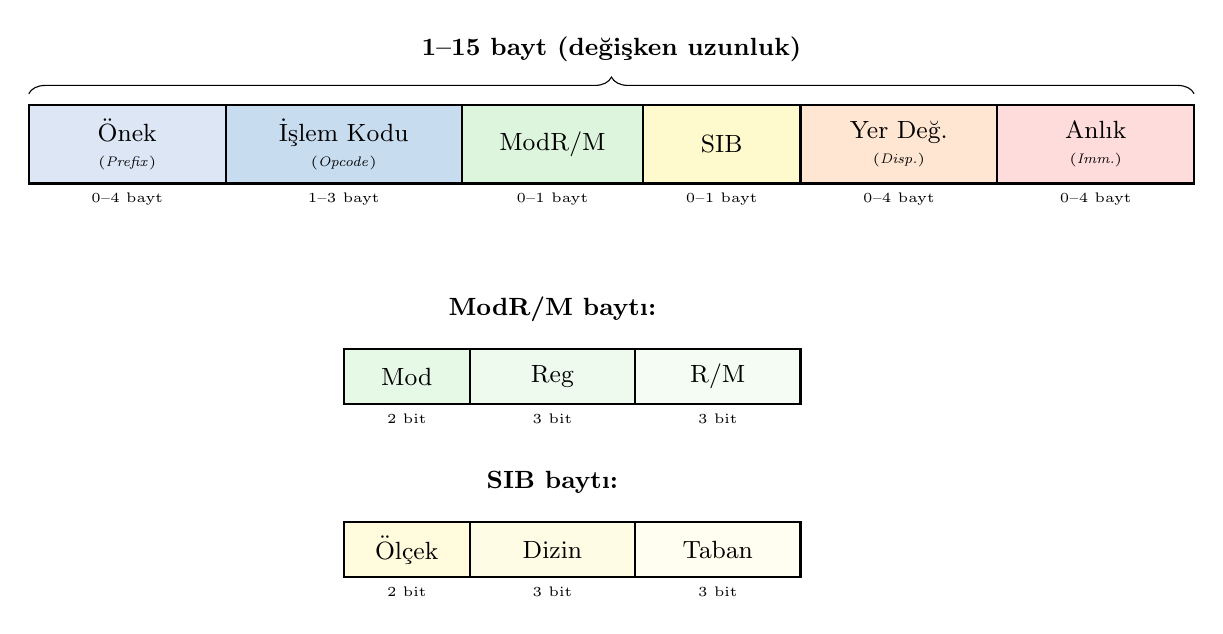
\begin{tikzpicture}[scale=1.0]
  \def\rh{1.0}  % satır yüksekliği

  % Renk tanımları
  \definecolor{cpfx}{RGB}{220, 230, 245}
  \definecolor{copc}{RGB}{200, 220, 240}
  \definecolor{cmodrm}{RGB}{220, 245, 220}
  \definecolor{csib}{RGB}{255, 250, 205}
  \definecolor{cdisp}{RGB}{255, 230, 210}
  \definecolor{cimmx}{RGB}{255, 220, 220}

  % Prefix (0--4 bayt)
  \draw[thick, fill=cpfx] (0, 0) rectangle (2.5, \rh);
  \node[font=\small, align=center] at (1.25, \rh/2) {Önek\\[-2pt]{\tiny (\textit{Prefix})}};
  \node[font=\tiny, below] at (1.25, 0) {0--4 bayt};

  % Opcode (1--3 bayt)
  \draw[thick, fill=copc] (2.5, 0) rectangle (5.5, \rh);
  \node[font=\small, align=center] at (4.0, \rh/2) {İşlem Kodu\\[-2pt]{\tiny (\textit{Opcode})}};
  \node[font=\tiny, below] at (4.0, 0) {1--3 bayt};

  % ModR/M (0--1 bayt)
  \draw[thick, fill=cmodrm] (5.5, 0) rectangle (7.8, \rh);
  \node[font=\small, align=center] at (6.65, \rh/2) {ModR/M};
  \node[font=\tiny, below] at (6.65, 0) {0--1 bayt};

  % SIB (0--1 bayt)
  \draw[thick, fill=csib] (7.8, 0) rectangle (9.8, \rh);
  \node[font=\small, align=center] at (8.8, \rh/2) {SIB};
  \node[font=\tiny, below] at (8.8, 0) {0--1 bayt};

  % Displacement (0--4 bayt)
  \draw[thick, fill=cdisp] (9.8, 0) rectangle (12.3, \rh);
  \node[font=\small, align=center] at (11.05, \rh/2) {Yer Değ.\\[-2pt]{\tiny (\textit{Disp.})}};
  \node[font=\tiny, below] at (11.05, 0) {0--4 bayt};

  % Immediate (0--4 bayt)
  \draw[thick, fill=cimmx] (12.3, 0) rectangle (14.8, \rh);
  \node[font=\small, align=center] at (13.55, \rh/2) {Anlık\\[-2pt]{\tiny (\textit{Imm.})}};
  \node[font=\tiny, below] at (13.55, 0) {0--4 bayt};

  % Üst parantez - değişken uzunluk
  \draw[decorate, decoration={brace, amplitude=6pt, raise=4pt}]
        (0, \rh) -- (14.8, \rh)
        node[midway, above=12pt, font=\small\bfseries] {1--15 bayt (değişken uzunluk)};

  % ModR/M detay (alt satır)
  \node[font=\small\bfseries] at (6.65, -1.6) {ModR/M baytı:};
  \draw[thick, fill=cmodrm!70] (4.0, -2.8) rectangle (5.6, -2.1);
  \node[font=\small] at (4.8, -2.45) {Mod};
  \node[font=\tiny, below] at (4.8, -2.8) {2 bit};
  \draw[thick, fill=cmodrm!50] (5.6, -2.8) rectangle (7.7, -2.1);
  \node[font=\small] at (6.65, -2.45) {Reg};
  \node[font=\tiny, below] at (6.65, -2.8) {3 bit};
  \draw[thick, fill=cmodrm!30] (7.7, -2.8) rectangle (9.8, -2.1);
  \node[font=\small] at (8.75, -2.45) {R/M};
  \node[font=\tiny, below] at (8.75, -2.8) {3 bit};

  % SIB detay
  \node[font=\small\bfseries] at (6.65, -3.8) {SIB baytı:};
  \draw[thick, fill=csib!70] (4.0, -5.0) rectangle (5.6, -4.3);
  \node[font=\small] at (4.8, -4.65) {Ölçek};
  \node[font=\tiny, below] at (4.8, -5.0) {2 bit};
  \draw[thick, fill=csib!50] (5.6, -5.0) rectangle (7.7, -4.3);
  \node[font=\small] at (6.65, -4.65) {Dizin};
  \node[font=\tiny, below] at (6.65, -5.0) {3 bit};
  \draw[thick, fill=csib!30] (7.7, -5.0) rectangle (9.8, -4.3);
  \node[font=\small] at (8.75, -4.65) {Taban};
  \node[font=\tiny, below] at (8.75, -5.0) {3 bit};
\end{tikzpicture}
\caption{x86'da Değişik Buyruk Biçimleri}
\label{fig:x86-buyruk-bicimleri}
\end{figure}


\subsection{Dört Mimarinin Genel Karşılaştırması}

Tablo~\ref{tab:dort-mimari-karsilastirma}'da RISC-V, MIPS, ARM ve x86 mimarileri temel özellikler açısından karşılaştırılmıştır.

\begin{table}[H]
\centering
\caption{RISC-V, MIPS, ARM ve x86 mimarilerinin karşılaştırması}
\label{tab:dort-mimari-karsilastirma}
\small
\begin{tabular}{lllll}
\toprule
\textbf{Özellik} & \textbf{RISC-V} & \textbf{MIPS} & \textbf{ARM (AArch64)} & \textbf{x86-64} \\
\midrule
Tür          & RISC       & RISC       & RISC       & CISC \\
Lisans       & Açık       & Ticari     & Ticari     & Ticari \\
Yazmaç sayısı & 32        & 32         & 31+ZR      & 16 \\
Buyruk boyutu & 32 bit    & 32 bit     & 32 bit     & Değişken \\
Bayt sırası  & Küçüğü başta & İkisi de & İkisi de  & Küçüğü başta \\
Anlık değer  & 12/20 bit  & 16/26 bit  & 12/16 bit  & 8/16/32 bit \\
Adresleme kipi & 4          & 3          & $\sim$6    & 10+ \\
Koşullu dallanma & beq, blt  & slt+beq   & NZCV kodları & FLAGS yazmacı \\
Çarpma/bölme & M uzantısı  & HI/LO     & Temel kümede & Temel kümede \\
Altyordam çağırma & jal (yazmaç) & jal (yazmaç) & BL (yazmaç) & CALL (yığıt) \\
Uzantı modeli & Modüler    & Sabit      & Profil tabanlı & Monolitik kümülatif \\
\bottomrule
\end{tabular}
\end{table}


% =====================================================
\section{Diğer Bazı Buyruk Kümesi Mimarileri}
\label{sec:diger-bkm}

Bilgisayar tarihi boyunca pek çok buyruk kümesi mimarisi tasarlanmıştır. Bu mimarilerin bir kısmı artık üretilmese de, her biri günümüz tasarımlarını etkileyen kavramsal katkılar yapmıştır. Tablo~\ref{tab:diger-bkm-ozet}'te bu mimarilerin özellikleri özetlenmiştir.

\begin{table}[H]
\centering
\caption{Bilgisayar tarihinde öne çıkan diğer buyruk kümesi mimarileri}
\label{tab:diger-bkm-ozet}
\footnotesize
\begin{tabular}{llclp{5.8cm}}
\toprule
\textbf{Mimari} & \textbf{Tasarımcı} & \textbf{Yıl} & \textbf{Tür} & \textbf{Öne çıkan özellik} \\
\midrule
System/360\index{System/360} & IBM & 1964 & CISC & İlk mimari aile kavramı; geriye uyumluluk geleneğini başlattı \\[2pt]
VAX\index{VAX} & DEC & 1977 & CISC & En zengin adresleme kipleri; RISC tartışmasının başlamasına neden oldu \\[2pt]
M68000\index{Motorola 68000} & Motorola & 1979 & CISC & İlk Macintosh ve Amiga işlemcisi; düzenli 32-bit tasarım \\[2pt]
SPARC\index{SPARC} & Sun & 1987 & RISC & Yazmaç penceresi kavramı; ilk açık kaynak BKM \\[2pt]
PA-RISC\index{PA-RISC} & HP & 1986 & RISC & VLIW kavramına geçiş deneyi (Itanium'un öncüsü) \\[2pt]
Power\index{Power Architecture} & IBM & 1990 & RISC & Sunucu ve süper bilgisayarlarda yaygın; POWER10 ile hâlâ üretimde \\[2pt]
Alpha\index{DEC Alpha} & DEC & 1992 & RISC & Döneminin en hızlı işlemcisi; 64-bit RISC öncüsü \\[2pt]
SuperH\index{SuperH} & Hitachi & 1992 & RISC & 16-bit sıkıştırılmış buyruklar; RISC-V C uzantısına ilham verdi \\
\bottomrule
\end{tabular}
\end{table}

Bu mimarilerin çoğu artık üretilmemektedir. Ancak katkıları yaşamaktadır: System/360'ın başlattığı geriye uyumluluk geleneği x86'da sürer, SPARC'ın açık kaynak yaklaşımı RISC-V'e ilham vermiştir, Alpha'nın 64-bit tasarım ilkeleri ARM AArch64 ve RISC-V RV64'te iz bırakmıştır.


% =====================================================
% Gerçek Dünya: Buyruk Kümesi Tasarım Kararları
% =====================================================
\section{Gerçek Dünya: Buyruk Kümesi Tasarım Kararları}
\label{sec:buyruk-gercek-dunya}

Buyruk kümesi tasarımı akademik bir konu olmaktan çok ötedir; endüstrideki her yeni mimari nesil, buyruk kümesi düzeyinde verilen kararların sonuçlarını taşır.

\subsubsection*{x86'nın geriye uyumluluk yükü}
Intel'in x86\index{x86} mimarisi 1978'den bu yana geriye uyumluluğu korur: günümüzün en güçlü Xeon işlemcisi bile 8086 için yazılmış bir programı çalıştırabilir. Bu esneklik muazzam bir ticari avantaj sağlasa da her nesil işlemciye ek karmaşıklık yükler. Çağdaş x86 işlemcileri, CISC buyrukları içeride RISC benzeri mikro-işlemlere çevirirken transistör bütçesinin önemli bir bölümünü bu dönüşüm birimine ayırır.

\subsubsection*{ARM'ın elde taşınır cihazlardaki hakimiyeti}
ARM\index{ARM} mimarisi, düşük güç tüketimi odaklı tasarımıyla akıllı telefonların neredeyse tamamında kullanılır. 2020'den itibaren Apple'ın M serisi işlemcilerle dizüstü ve masaüstü pazarına girmesi, ARM'ın ``yalnızca düşük güçlü cihazlar için'' algısını kökten değiştirdi. ARM'ın lisanslama modeli, farklı şirketlerin aynı buyruk kümesi üzerinde kendi mikromimarilerini tasarlamasına olanak tanır.

\begin{bilginot}[Neden Elde Taşınır Cihazlarda x86 Yok?]
\index{x86!elde taşınır cihazlar}\index{ARM!elde taşınır cihazlar}
Akıllı telefonlar, tabletler ve giyilebilir cihazlar neredeyse tamamıyla ARM tabanlı işlemcilerle çalışır. Intel, 2012--2016 yılları arasında Atom işlemci ailesiyle bu pazara girmeye çalışmış, hatta telefon üreticilerine mali destek sunmuş, ancak başarılı olamamıştır. Bunun temel nedenleri buyruk kümesi mimarisinin doğasında yatmaktadır:

\begin{enumerate}[nosep]
\item \emph{Güç verimliliği:} x86'nın karmaşık, değişken uzunluklu buyrukları her saat döngüsünde mikro-işlemlere çözülür; bu dönüşüm birimi sürekli güç harcar. ARM'ın sabit uzunluklu, basit buyrukları çok daha az enerjiyle çözülebilir. Pille çalışan bir cihazda her miliwatt değerlidir.
\item \emph{Çözme karmaşıklığı:} x86'da buyruk uzunluğu 1 ile 15 bayt arasında değişir; bu durum çözme donanımını büyütür ve ısı üretimini artırır. ARM ve RISC-V'te sabit 4 baytlık buyruklar koşut çözmeyi kolaylaştırır.
\item \emph{Transistör bütçesi:} x86'nın geriye uyumluluk yükü, transistörlerin önemli bir bölümünü ``eski buyrukları destekleme'' için harcar. ARM tasarımları bu bütçeyi daha fazla çekirdeğe veya daha büyük önbelleğe ayırabilir.
\item \emph{Lisanslama esnekliği:} ARM, BKM lisansını satarak farklı şirketlerin (Apple, Qualcomm, Samsung) aynı buyruk kümesi üzerinde kendi mikromimarilerini tasarlamasına olanak tanır. Intel ise hem BKM'yi hem üretimi kendi elinde tuttuğundan, cihaz üreticilerine bu esnekliği sunamaz.
\end{enumerate}

Apple'ın 2020'de kendi ARM tabanlı M1 işlemcisiyle dizüstü bilgisayar pazarına girmesi, bu esnekliğin gücünü göstermiştir. M1'den M5'e uzanan bu yonga ailesi, her kuşakta aynı güç zarfında x86 rakiplerini geride bırakmaya devam etmektedir.
\end{bilginot}

\subsubsection*{RISC-V'in yükselişi}
RISC-V\index{RISC-V}'nin açık kaynak doğası, onu özellikle gömülü sistemlerde, akademik araştırmalarda ve Çin'in yarı iletken endüstrisinde hızla benimsenen bir seçenek haline getirdi. SiFive, Alibaba (Xuantie serisi) ve Bouffalo Lab gibi şirketler ticari RISC-V işlemcileri üretmektedir.

2025 yılında Meta'nın RISC-V tabanlı sunucu işlemcisi geliştiren RIVOS şirketini satın alması, RISC-V'in gömülü sistemlerin ötesine geçerek veri merkezi pazarına girişinin somut bir göstergesi olmuştur. Bu satın alma, dünyanın en büyük veri merkezi işletmecilerinden birinin ARM ve x86'ya seçenek olarak RISC-V'e yatırım yaptığını göstermekte ve açık kaynak buyruk kümesi mimarisinin sunucu düzeyinde rekabet edebileceği mesajını vermektedir.

\subsubsection*{Veri koşutluğu ve BKM uzantıları}
\index{SIMD}\index{vektör uzantıları}
İşlemcilerin aynı anda birden fazla veri üzerinde aynı işlemi yapabilmesi (\emph{Single Instruction, Multiple Data}, SIMD\index{SIMD}) kavramı, buyruk kümelerinin evriminde belirleyici bir rol oynamıştır. Bu uzantılar, multimedya işleme, bilimsel hesaplama ve yapay zekâ iş yüklerindeki veri koşutluğunu donanım düzeyinde destekler.

x86 mimarisinde bu evrim kümülatif biçimde ilerlemiştir:
\begin{itemize}[nosep]
\item \textbf{MMX}\index{MMX} (1997): 64 bitlik yazmaçlarla 8 adet 8 bitlik tam sayı işlemi; multimedya odaklı ilk adım.
\item \textbf{SSE}\index{SSE} (1999): 128 bitlik \texttt{xmm} yazmaçları; 4 adet tek duyarlıklı kayan nokta işlemi koşut olarak yürütülür.
\item \textbf{AVX}\index{AVX} (2011): 256 bitlik \texttt{ymm} yazmaçları; veri genişliği iki katına çıkar.
\item \textbf{AVX-512}\index{AVX-512} (2017): 512 bitlik \texttt{zmm} yazmaçları; 16 adet tek duyarlıklı kayan nokta işlemi tek buyrukla yapılır.
\end{itemize}

Her yeni uzantı öncekini kapsadığından, x86 işlemcileri tüm eski SIMD buyruklarını da desteklemek zorundadır; bu da geriye uyumluluk yükünü artırır.

ARM mimarisi benzer gereksinime farklı yanıt vermiştir. NEON\index{NEON} uzantısı (128 bit) sabit genişlikteyken, SVE\index{SVE} (\emph{Scalable Vector Extension}) ve onun geliştirilmiş sürümü SVE2 değişken vektör uzunluğu sunar: aynı buyruk, 128 bitten 2048 bite kadar farklı genişliklerde çalışabilir. Bu yaklaşım, yazılımın donanımdan bağımsız olmasını sağlar.

RISC-V ``V'' (vektör) uzantısı\index{RISC-V!V uzantısı} ise en esnek modeli sunar. Vektör uzunluğu buyruk kümesinde sabitlenmez; donanım ne kadar geniş vektör birimi sağlıyorsa yazılım o kadarını kullanır. Bu tasarım, küçük bir gömülü işlemcide 64 bitlik, yüksek başarımlı bir sunucuda 1024 bitlik vektörlerle aynı programın çalışmasını mümkün kılar.

\subsubsection*{Yapay zekâ çağında buyruk kümesinin dönüşümü}
\index{yapay zekâ!buyruk kümesi etkisi}
Yapay zekâ iş yükleri, buyruk kümesi tasarımını köklü biçimde etkilemektedir. Geleneksel hesaplama 32 veya 64 bitlik kayan nokta duyarlığı gerektirirken, sinir ağı çıkarımı çok daha düşük duyarlıkla çalışabilir. Bu gereksinim, buyruk kümelerine yeni veri türleri ve özel buyruklar eklenmesine yol açmıştır:

\begin{itemize}[nosep]
\item \textbf{Düşük duyarlıklı veri türleri:} INT8, FP16 ve BF16 (\emph{bfloat16}) gibi dar veri türleri, aynı bant genişliğiyle iki veya dört kat daha fazla veri işlemeyi mümkün kılar. Intel AMX\index{AMX} (\emph{Advanced Matrix Extensions}), ARM SME\index{SME} (\emph{Scalable Matrix Extension}) ve RISC-V'in önerilen matris uzantıları bu veri türlerini doğrudan destekler.
\item \textbf{Matris buyrukları:} Sinir ağlarının temelindeki matris çarpımı, geleneksel skaler veya SIMD buyrukları yerine özel matris birimlerinde çok daha verimli yürütülür. Google TPU\index{TPU}, bu yaklaşımın en uç örneğidir: buyruk kümesinin tamamı matris işlemlerine odaklanmıştır.
\item \textbf{Alana özgü hızlandırıcılar:} Sinir ağı motoru (NPU\index{NPU}) artık birçok yonganın standart bileşenidir (Apple Neural Engine, Qualcomm Hexagon). Bu birimler BKM'den bağımsız yan işlemci olarak çalışır; ancak bazıları ana BKM'den özel buyrukla tetiklenir.
\end{itemize}

RISC-V'in bu dönüşümde öne çıkmasının nedeni, şirketlerin standart buyruk kümesine kendi özel YZ uzantılarını ekleyebilmesidir. Ticari mimarilerde böyle bir esneklik yoktur; x86 veya ARM kullanıcısı, üretici firmanın sunduğu uzantılarla yetinmek zorundadır. Bu esneklik, RISC-V'i YZ hızlandırıcılarının giderek daha çok tercih ettiği bir temel haline getirmektedir.


% =====================================================
% Yanılgılar ve Tuzaklar
% =====================================================
\section{Yanılgılar ve Tuzaklar}
\label{sec:buyruk-yanilgilar}

Buyruk kümesi mimarisi, sezgisel olarak basit görünse de öğrencilerin sık düştüğü tuzaklar içerir.

\yanilgi{Daha fazla buyruk türü olan mimari daha güçlüdür}
CISC mimarilerinin zengin buyruk kümesi, her buyruğun eşit sıklıkta kullanıldığı anlamına gelmez. x86'nın yüzlerce buyruğunun büyük çoğunluğu derleyiciler tarafından nadiren üretilir. RISC felsefesi, az sayıda ama sık kullanılan buyruğu hızlı çalıştırmanın daha verimli olduğunu göstermiştir.

\yanilgi{Yazmaç sayısı arttıkça başarım her zaman artar}
Daha fazla yazmaç, derleyiciye daha fazla esneklik sunar; ancak her ek yazmaç, buyruk kodlamasında daha fazla bit gerektirir (RISC-V'te 5 bit = 32 yazmaç). Yazmaç sayısının artması buyruk boyutunu büyütür, bu da buyruk önbelleğinde daha fazla yer kaplar ve bellek bant genişliğini tüketir.

\yanilgi{Sabit uzunluklu buyruklar her zaman değişken uzunlukludan iyidir}
RISC-V ve MIPS gibi mimarilerde 32 bitlik sabit buyruk uzunluğu, kod çözmeyi basitleştirir. Ancak bu, kod yoğunluğunu azaltır; aynı program daha fazla bellek kaplar. ARM'ın Thumb-2 modu ve RISC-V'in ``C'' (sıkıştırılmış) uzantısı, 16 bitlik kısa buyruklar ekleyerek bu sorunu hafifletir.

\tuzak{Küçüğü başta ve büyüğü başta sıralamasını karıştırmak}
Ağ üzerinden veri aktarımında genellikle büyüğü başta (big-endian) sıralama kullanılırken, x86 ve RISC-V küçüğü başta (little-endian) kullanır. Farklı sıralamaya sahip sistemler arasında veri aktarırken bayt sırası dönüştürülmezse veriler bozulur. Bu, özellikle gömülü sistem ve ağ programlamada sık karşılaşılan bir hatadır.

\tuzak{İşaret uzatmasını göz ardı etmek}
\texttt{lb} buyruğu bellekten okuduğu 8 bitlik değeri 32 bite işaret uzatarak yazar; en yüksek değerlikli bit~1 ise yazmaç \texttt{0xFFFFFFxx} biçiminde dolar. İşaretsiz bir değer okunmak isteniyorsa \texttt{lbu} kullanılmalıdır. Aynı durum \texttt{lh}/\texttt{lhu} çifti için de geçerlidir. Bu ayrımın gözden kaçması, özellikle karakter işleme ve görüntü verisi gibi işaretsiz bayt dizileriyle çalışırken bulunması güç hatalara yol açar.

\tuzak{Anlık değerin 12 bitlik sınırını aşmak}
I-tipi buyruklardaki anlık alan yalnızca 12 bittir ve $-2048$ ile $+2047$ arasında değer taşıyabilir. Bu sınırı aşan bir sabiti doğrudan \texttt{addi} ile yüklemek derleme hatasına neden olur. Büyük sabitler için önce \texttt{lui} ile üst 20 bit, ardından \texttt{addi} ile alt 12 bit yüklenir. Çevirici, \texttt{li} sözde buyruğunu tam da bu iki gerçek buyruğa dönüştürerek programcıyı bu ayrıntıdan kurtarır; ancak üretilen kodun iki buyruk yer kapladığını bilmek, döngü gövdelerinde buyruk sayısını tahmin ederken önemlidir.

\tuzak{Çağıran ve çağrılan taraf yazmaçlarını karıştırmak}
RISC-V çağırma alışkanlığında \texttt{s0}--\texttt{s11} yazmaçları çağrılan tarafça saklanır; altyordam bu yazmaçları kullanıyorsa giriş kodunda yığıta yazıp çıkış kodunda geri yüklemelidir. Buna karşılık \texttt{t0}--\texttt{t6} geçici yazmaçları çağıran tarafın sorumluluğundadır ve altyordam bunları serbestçe bozabilir. Bu ayrımı karıştırmak, altyordam dönüşünde beklenmeyen yazmaç değerlerine ve izlenmesi güç hatalara yol açar.

\yanilgi{Sözde buyruklar donanımda ayrı buyruklardır}
\texttt{mv}, \texttt{li}, \texttt{nop}, \texttt{j} gibi sözde buyruklar programcının işini kolaylaştıran kısaltmalardır; donanımda ayrı bir işlem kodu yoktur. Çevirici bunları gerçek buyruklara dönüştürür: \texttt{mv rd, rs1} $\to$ \texttt{addi rd, rs1, 0}; \texttt{nop} $\to$ \texttt{addi x0, x0, 0}; \texttt{j etiket} $\to$ \texttt{jal x0, etiket}. Sözde buyrukları ``gerçek'' sanmak, buyruk sayma ve kodlama sorularında hatalı sonuçlara götürür.


% =====================================================
\section{Özet}
\label{sec:bolum3-ozet}

Bu bölümde bilgisayarın ``ana dilini'', yani buyruk kümesi mimarisini, öğrendik. Bilgisayarlar yalnızca 0 ve 1'lerle çalışır; yazılım ile donanım arasındaki köprüyü buyruk kümesi kurar. Karmaşık buyrukları destekleyen mimariler CISC\index{CISC}, yalın buyrukları destekleyen mimariler ise RISC\index{RISC} olarak adlandırılır.

Bu kitapta kullandığımız RISC-V, UC Berkeley'de 2010 yılında tasarlanmış açık kaynaklı bir RISC buyruk kümesi mimarisidir. Modüler yapısı sayesinde RV32I temel buyruk kümesinin üzerine M, A, F, D, C gibi uzantılar eklenerek işlemci gereksinime göre özelleştirilebilir.

RISC-V'in 32 tamsayı yazmacı, işlemcinin en hızlı saklama birimleridir; sık kullanılan veriler yazmaçlarda tutularak bellek erişimi azaltılır. Yazmaçların yetersiz kaldığı durumlarda derleyici bazı değerleri yığıta yazarak yazmaçtan belleğe taşıma yapar.

Bir programcının gereksinim duyduğu temel buyruk türleri (aritmetik, mantık, veri aktarımı, kaydırma ve dallanma) RISC-V'te altı biçimde (R, I, S, B, U, J) kodlanır. Bu buyruklar, verilerine yazmaç, anlık, eklemeli (taban), PS'ye göreceli ve üst anlık gibi farklı adresleme kipleriyle erişir. Çevirici, \texttt{mv}, \texttt{li}, \texttt{nop} gibi sözde buyrukları gerçek buyruklara dönüştürerek programcıya kolaylık sağlar; bu sözde buyruklar donanımda ayrı bir işlem koduna karşılık gelmez.

Altyordamlar, kodun yeniden kullanılmasını sağlayan temel yapı taşlarıdır. RISC-V'te \texttt{jal} ile altyordam çağrılır, \texttt{jalr} ile geri dönülür. İç içe çağrılarda dönüş adresi ve saklanması gereken yazmaçlar yığıta yazılır. Çağırma alışkanlıkları, hangi yazmaçların çağıran, hangilerinin çağrılan tarafça saklanacağını belirleyerek yazılım modüllerinin birbirinden bağımsız biçimde derlenmesini olanaklı kılar.

Bir programın yürütülebilir dosyaya dönüşme süreci dört aşamadan oluşur: derleyici üst düzey dili çeviriye dönüştürür, çevirici bunu nesne dosyasına çevirir, bağlayıcı nesne dosyalarını ve kütüphaneleri birleştirerek yürütülebilir dosyayı oluşturur, yükleyici ise bu dosyayı belleğe yerleştirir. Bellekteki program, metin (.text), veri (.data, .bss), yığın (heap) ve yığıt (stack) bölgelerine ayrılır.

RISC-V, MIPS, ARM ve x86 mimarileri farklı tasarım felsefelerini yansıtır. RISC-V ve MIPS sabit uzunluklu buyruk ve yük-sakla modeliyle yalınlığı öncelerken, x86 değişken uzunluklu buyruklar ve bellek-yazmaç işlemleriyle geriye uyumluluğu korur. ARM ise koşullu yürütme ve esnek kaydırıcı gibi özellikleriyle ikisinin arasında bir noktada durur.

Bu bölümde ele alınan kavramlar, bilgisayar mimarisinde izlenen dört ana ilkeyi somutlaştırır:
\begin{sloppypar}
\begin{enumerate}
\item \textbf{Olağan durumu hızlandır:} Sık kullanılan buyruklar kısa ve hızlı tasarlanır; ``C'' uzantısı en yaygın buyrukları 16 bite sıkıştırarak kod yoğunluğunu artırır.
\item \textbf{Yalınlık düzenden gelir:} Sabit uzunluklu buyruk biçimi ve düzenli yazmaç alanları, donanımda kod çözme devresini yalınlaştırır.
\item \textbf{Küçük olan hızlıdır:} 32 yazmaçlık dosya, binlerce adresli bellekten çok daha hızlı erişilebilir; bu nedenle sık kullanılan veriler yazmaçlarda tutulur.
\item \textbf{İyi tasarım ödünleşme gerektirir:} Yazmaç sayısı, buyruk uzunluğu ve adresleme kipi çeşitliliği arasındaki denge, mimari tasarımın temel ödünleşmesidir.
\end{enumerate}

\end{sloppypar}

% =====================================================
\section*{Alıştırmalar}
\addcontentsline{toc}{section}{Alıştırmalar}

\begin{alistirma}[\kolay]
Aşağıdaki ikilik tabanda verilmiş olan sayıları onluk tabana çevirin.\\
(a) $(10111001100)_2$ \quad (b) $(111010)_2$ \quad (c) $(1000111)_2$
\end{alistirma}

\begin{alistirma}[\kolay]
Onluk tabanda verilmiş olan sayıları ikilik tabana çevirin.\\
(a) $(128)_{10}$ \quad (b) $(14)_{10}$ \quad (c) $(557)_{10}$
\end{alistirma}

\begin{alistirma}[\orta]
Aşağıdaki ikilik tabandaki dört işlem alıştırmalarını çözün.\\
(a) $1001100 + 111011 = ?$ \quad (b) $111001 - 100111 = ?$\\
(c) $110011 \div 110 = ?$ \quad (d) $101 \times 111 = ?$
\end{alistirma}

\begin{alistirma}[\kolay]
İşlemcide buyrukların geçtiği aşamalar nelerdir? Bir buyruğun işlemci içindeki ömründe sırasıyla hangi işlemlerin yapılması gerekir?
\end{alistirma}

\begin{alistirma}[\kolay]
İkiye tümleyen aritmetiğinin bire tümleyen ve işaretli büyüklük gösterim biçimlerine göre üstünlüğü nedir?
\end{alistirma}

\begin{alistirma}[\orta]
İşlemcilerde eksi sayılar nasıl gösterilir? $-8$ sayısını göstermek için değişik gösterim yöntemlerinde kaç bit gerekir?
\end{alistirma}

\begin{alistirma}[\kolay]
``Küçüğü Başta'' ve ``Büyüğü Başta'' terimlerini açıklayın.
\end{alistirma}

\begin{alistirma}[\orta]
İşlemcilerde kullanılan adresleme yöntemlerini yazarak bu yöntemlerin nasıl çalıştığını açıklayın. RISC-V'te yükleme ve saklama işlemlerinin yapılması için hangi adresleme yöntemi kullanılır?
\end{alistirma}

\begin{alistirma}[\orta]
$(4A3B2C1D)_{16}$ sözcüğünün bellekte küçüğü başta ve büyüğü başta yöntemlerini kullanan iki ayrı işlemcide nasıl durduğunu gösterin.
\end{alistirma}

\begin{alistirma}[\kolay]
Yazmaç türlerini açıklayın.
\end{alistirma}

\begin{alistirma}[\orta]
RISC-V mimarisinde buyruklar kaç bit ile ifade edilir? Intel x86 mimarisinde buyruk yapıları nasıldır? Açıklayın.
\end{alistirma}

\begin{alistirma}[\orta]
RISC-V buyruk kümesi mimarisinde kaç tür buyruk biçimi vardır? Bu buyruk biçimlerini açıklayın.
\end{alistirma}

\begin{alistirma}[\kolay]
Java, C gibi üst düzey bir programlama dilinde yazılmış bir kod parçasının bilgisayar tarafından çalıştırılmasına kadar geçtiği evreleri açıklayın.
\end{alistirma}

\begin{alistirma}[\kolay]
Derleyicilerin kullanım amaçları ve programcılara sağladığı avantajları açıklayın.
\end{alistirma}

\begin{alistirma}[\orta]
Dört tasarım ilkesini örnek vererek açıklayın: (a) Olağan durumu hızlandır, (b) Yalınlık düzenden gelir, (c) Küçük olan hızlıdır, (d) İyi tasarım için ödünleşme gerekir.
\end{alistirma}

\begin{alistirma}[\kolay]
Yapılan işlemlerin işleçlerinin ve sonucunun yazmaçlarda tutulmasının amacı nedir?
\end{alistirma}

\begin{alistirma}[\orta]
RISC-V mimarisinde 32 yazmaç bulunur. Bir programda 32'den fazla sayıda değişken bulunduğunda ne olur?
\end{alistirma}

\begin{alistirma}[\orta]
RISC-V'te çarpma işleminin sonucu nereye yazılır? MIPS'teki HI ve LO yazmaçları ile RISC-V'in yaklaşımını karşılaştırın.
\end{alistirma}

\begin{alistirma}[\kolay]
RISC-V'te bir yazmacın değerini başka bir yazmaca kopyalamak için hangi buyruk kullanılır? Bu işlemi gerçekleştiren kodu yazın.
\end{alistirma}

\begin{alistirma}[\kolay]
Sözcüklerin bellekte hizalanmış olarak durması ne demektir? RISC-V'te sözcükler bellekte nasıl durur?
\end{alistirma}

\begin{alistirma}[\orta]
Buyruk kümesinde daha fazla genel amaçlı yazmaç olması neden iyidir? Yazmaç sayısı çok düşük olursa ne tür sorunlar ortaya çıkar? Yazmaç sayısının çok yüksek olmasının ne tür yan etkileri olabilir?
\end{alistirma}

\begin{alistirma}[\orta]
RISC-V'te program sayacına her vuruşta 4 eklenmesinin nedeni nedir? Intel'in x86 tabanlı işlemcilerinde program sayacına her vuruşta kaç eklenir?
\end{alistirma}

\begin{alistirma}[\orta]
RISC-V'te \texttt{blt} buyruğunun MIPS'teki \texttt{slt} ve \texttt{bne} buyruk çiftiyle karşılaştırıldığında sağladığı avantajı açıklayın.
\end{alistirma}

\begin{alistirma}[\orta]
RISC-V'in modüler buyruk kümesi mimarisinin avantajlarını açıklayın. RV32I temel buyruk kümesine M, F ve D uzantılarının eklenmesi ne tür işlevsellik kazandırır?
\end{alistirma}

\begin{alistirma}[\zor]
RISC-V, MIPS, ARM ve x86 mimarilerini buyruk boyutu, yazmaç sayısı, adresleme kipleri ve lisans modeli açısından karşılaştırın.
\end{alistirma}

\begin{alistirma}[\kolay]
Aşağıdaki sözde buyrukların her birinin hangi gerçek RISC-V buyruğuna (veya buyruklarına) dönüştürüldüğünü yazın: (a) \texttt{mv t0, t1} \quad (b) \texttt{li t0, 42} \quad (c) \texttt{j etiket} \quad (d) \texttt{not t0, t1} \quad (e) \texttt{nop}
\end{alistirma}

\begin{alistirma}[\orta]
\texttt{x = x * 32;} ifadesi için derleyici neden \texttt{mul} yerine kaydırma buyruğu üretir? Hangi 2'nin kuvvetleri için bu dönüşüm geçerlidir? RISC-V kodunu yazın.
\end{alistirma}

\begin{alistirma}[\orta]
RISC-V'te \texttt{dizi[i]} ifadesine erişmek için 3 buyruk gerekirken x86'da tek buyrukla (\texttt{mov eax, [ebx+ecx*4]}) erişilebilir. Bu durumda RISC-V neden daha az adresleme kipi sunmayı tercih etmiştir? Donanım karmaşıklığı, saat sıklığı ve boru hattı tasarımı açısından tartışın.
\end{alistirma}

\begin{alistirma}[\orta]
32 bitlik \texttt{0xABCD1234} sabitini bir RISC-V yazmacına yüklemek için gereken buyruk dizisini yazın. \texttt{lui} ve \texttt{addi} buyruklarının her birinin yazmacı nasıl değiştirdiğini adım adım gösterin.
\end{alistirma}

%% ===================================================================
%% Aşağıdaki sorular BİL 361 dersinin geçmiş yıllardan sınav
%% sorularından uyarlanmıştır.
%% ===================================================================

\begin{alistirma}[\orta]
Aşağıdaki RISC-V buyruk türleri için birer örnek buyruk yazın ve her birinin bit düzenini (opcode, funct3, funct7, rs1, rs2, rd, imm alanları) gösterin: (a) R tipi, (b) I tipi, (c) S tipi.
\end{alistirma}

\begin{alistirma}[\zor]
Aşağıda C dilinde yazılmış bir fonksiyonun RISC-V çevirici dilindeki karşılığını yazın. Yazmaç kullanımını açıkça belirtin.
\begin{lstlisting}[language=C, style=alistirma-kod]
int fib(int n) {
    if (n == 0 || n == 1)
        return n;
    return fib(n - 1) + fib(n - 2);
}
\end{lstlisting}
\end{alistirma}

\begin{alistirma}[\zor]
Aşağıdaki RISC-V çevirici dil kodunun ne iş yaptığını açıklayın. \texttt{x1} yazmacının başlangıç değeri $N$ olduğuna göre, program sona erdiğinde \texttt{x6} yazmacındaki değer nedir?
\begin{lstlisting}[style=riscv, style=alistirma-kod]
    addi x2, x0, 0x8000
    addi x4, x0, 1
    addi x5, x0, 0
dongu:
    ld   x8, 0(x2)
    ld   x9, 8(x2)
    add  x2, x0, x9
    mul  x4, x4, x8
    addi x5, x5, 1
    blt  x5, x1, dongu
    add  x6, x0, x4
\end{lstlisting}
\end{alistirma}

\begin{alistirma}[\zor]
Döngünün açılması (\emph{loop unrolling}) yöntemi hakkında aşağıdaki soruları yanıtlayın:
\begin{enumerate}[(a)]
    \item Aşağıdaki döngüyü 4 kere açın ve açılmış halini yazın:
\begin{lstlisting}[language=C, style=alistirma-kod]
for (int i = 0; i < 15000000; i++) {
    b[i] = a[i];
    if (i % 2 == 0) c[i] = d[i];
}
\end{lstlisting}
    \item Açılmamış ve açılmış döngülerin durağan (\emph{static}) ve devingen (\emph{dynamic}) buyruk sayılarını karşılaştırın.
    \item Döngünün açılmasının buyruk önbelleği başarımına olası etkisini tartışın.
\end{enumerate}
\end{alistirma}

\begin{alistirma}[\zor]
Aşağıdaki buyruk kümesi tablosu verilmiştir. Bu buyrukları kullanarak, belleğin \texttt{0x1000} adresinden başlayan 64 elemanlı $A$ dizisi ile \texttt{0x2000} adresinden başlayan 64 elemanlı $B$ dizisinin eleman eleman toplamından oluşan, \texttt{0x3000} adresinden başlayan bir $C$ dizisi oluşturan çevirici dil programını yazın. Her eleman 4 bayttır.

\begin{center}
\begin{tabular}{|l|l|}
\hline
\textbf{Buyruk} & \textbf{Açıklama} \\ \hline
\texttt{topla rt, rs, rd} & \texttt{rt = rs + rd} \\ \hline
\texttt{cikar rt, rs, rd} & \texttt{rt = rs - rd} \\ \hline
\texttt{mov rt, anlık} & \texttt{rt $\leftarrow$ SıfırlaGenişlet(anlık)} \\ \hline
\texttt{bg rt, rs, anlık} & \texttt{rt > rs ise PS = PS + İşaretleGenişlet(anlık)} \\ \hline
\texttt{lw rt, rs} & \texttt{rt $\leftarrow$ Bellek[rs]} \\ \hline
\texttt{sw rt, rs} & \texttt{Bellek[rt] $\leftarrow$ rs} \\ \hline
\end{tabular}
\end{center}
\end{alistirma}

\begin{alistirma}[\zor]
Bir işlemci tasarımı projesi için buyruk kümesi tasarlanacaktır. Bu proje için tasarlanan mimarinin aşağıdaki özellikleri sağlaması beklenmektedir:
\begin{itemize}
    \item 16 adet genel kullanıma ayrılmış yazmaç vardır.
    \item İlk yazmaç her zaman sıfırdır.
    \item 4\,KB veri ve 4\,KB buyruk belleği mevcuttur.
    \item Bayt adresleme kullanılmaktadır.
    \item Desteklenmesi istenen buyruklar:
    \begin{itemize}
        \item \textbf{Topla:} İki yazmaç değerini toplar ve başka bir yazmaca yazar.
        \item \textbf{Çıkar:} İlk kaynak yazmaçtan ikinci kaynak yazmacın değerini çıkarır ve belirtilen yazmaca yazar.
        \item \textbf{ToplaVeYaz:} İki kaynak yazmacın değerini toplar ve ilk kaynak yazmaca yazar.
        \item \textbf{ÇıkarVeYaz:} İlk kaynak yazmaçtan ikinci kaynak yazmacın değerini çıkarır ve ilk kaynak yazmaca yazar.
        \item \textbf{Değiştir:} İki kaynak yazmacın değerlerini birbiriyle değiştirir.
        \item \textbf{Sakla:} Kaynak yazmaçtaki değeri anlık değerle verilen bellekteki adrese yazar.
        \item \textbf{Yükle:} Bellekte anlık değerle adreslenen veriyi hedef yazmacına yazar.
        \item \textbf{EşitseAtla:} İki kaynak yazmaçtaki değer birbirine eşitse program sayacının o anki değerine anlık değer eklenerek atlama gerçekleştirilir. Bu buyrukla en fazla $2^{20}$ bayt geri ya da $2^{20}-1$ bayt ileri gidilebilir. (Anlık değer 2'ye tümleyen biçimindedir.)
    \end{itemize}
\end{itemize}
\begin{enumerate}[(a)]
    \item Buyrukların sabit uzunlukta olduğu kabul edilirse:
    \begin{enumerate}[(i)]
        \item Buyruk uzunluğu en az kaç bittir?
        \item Bu özellikleri sağlayan buyruklar kaç farklı buyruk tipinden oluşmaktadır? Her buyruk tipini gösterin.
    \end{enumerate}
    \item Buyruk uzunlukları sabit olmasaydı tasarımınızda ne değişirdi?
    \item Bu tasarım tamamlandığında \texttt{topla} ve \texttt{çıkar} buyrukları için özel iyileştirmeler yapılmış ve BBÇ'leri düşürülmüştür. Yapılan benzetimler sonucu tüm buyrukların BBÇ'lerinin aşağıda verildiği gibi olduğu gözlemlenmiştir. Bu buyrukların oranlarının verildiği bir kodda derleme zamanında yapılacak iyileştirmelerle başarımı artırmanız istenmektedir. Başarımı artırmak için neler yapabilirsiniz? Bu iyileştirmeler sonucunda başarım başlangıca göre ne kadar artar?

    \begin{center}
    \footnotesize
    \begin{tabular}{|l|c|c|c|c|c|c|c|c|}
    \hline
     & \textbf{Topla} & \textbf{Çıkar} & \textbf{TopVeYaz} & \textbf{ÇıkVeYaz} & \textbf{Değiştir} & \textbf{Sakla} & \textbf{Yükle} & \textbf{EşitseAtla} \\ \hline
    \textbf{BBÇ} & 1 & 1 & 3 & 3 & 5 & 10 & 10 & 4 \\ \hline
    \textbf{\%} & 5 & 5 & 20 & 20 & 20 & 5 & 5 & 20 \\ \hline
    \end{tabular}
    \normalsize
    \end{center}

    (Yazmaç sayısının bu iyileştirmeler sırasında yeterli olacağını varsayabilirsiniz.)
    \item Bu buyruk kümesi mimarisini gerçekleyen işlemciyi çizip denetim tablosunu oluşturun.
\end{enumerate}
\end{alistirma}

\begin{alistirma}[\zor]
Aşağıda bir C programının küçük bir parçası verilmiştir. Bu program için derleyici tarafından üretilmesini beklediğiniz RISC-V çevirici dil kodunu yazın. Kodun hedefi RV32-IM mimarisidir. \texttt{fonk} fonksiyonu bellekte \texttt{0x2000} adresine, \texttt{carp} fonksiyonu ise \texttt{0x1600} adresine yerleştirilmelidir. RISC-V çağrı alışkanlıkları (\emph{calling convention}) kurallarına uygun bir çözüm yazın.

\begin{lstlisting}[language=C, style=alistirma-kod]
int carp(int a, int b, int c, int d, int e)
{
    return a * b * c * d * e;
}

int fonk(int x, int y)
{
    int z = carp(x, y, x, y, x);
    if (z < 150)
        return 0;
    else
        return 1;
}
\end{lstlisting}

\begin{enumerate}[(a)]
    \item Kodun neden belleğe saçılması gerekir? Kısa açıklayın.
    \item Her iki fonksiyon için RISC-V çevirici dil kodunu yazın. Yığıt (\emph{stack}) kullanımına ve çağıran/çağrılan (\emph{caller/callee}) yazmaç saklama kurallarına dikkat edin.
\end{enumerate}
\end{alistirma}
